% Options for packages loaded elsewhere
\PassOptionsToPackage{unicode}{hyperref}
\PassOptionsToPackage{hyphens}{url}
%
\documentclass[
  12pt,
]{article}
\usepackage{lmodern}
\usepackage{amsmath}
\usepackage{ifxetex,ifluatex}
\ifnum 0\ifxetex 1\fi\ifluatex 1\fi=0 % if pdftex
  \usepackage[T1]{fontenc}
  \usepackage[utf8]{inputenc}
  \usepackage{textcomp} % provide euro and other symbols
  \usepackage{amssymb}
\else % if luatex or xetex
  \usepackage{unicode-math}
  \defaultfontfeatures{Scale=MatchLowercase}
  \defaultfontfeatures[\rmfamily]{Ligatures=TeX,Scale=1}
  \setmainfont[]{Times New Roman}
\fi
% Use upquote if available, for straight quotes in verbatim environments
\IfFileExists{upquote.sty}{\usepackage{upquote}}{}
\IfFileExists{microtype.sty}{% use microtype if available
  \usepackage[]{microtype}
  \UseMicrotypeSet[protrusion]{basicmath} % disable protrusion for tt fonts
}{}
\makeatletter
\@ifundefined{KOMAClassName}{% if non-KOMA class
  \IfFileExists{parskip.sty}{%
    \usepackage{parskip}
  }{% else
    \setlength{\parindent}{0pt}
    \setlength{\parskip}{6pt plus 2pt minus 1pt}}
}{% if KOMA class
  \KOMAoptions{parskip=half}}
\makeatother
\usepackage{xcolor}
\IfFileExists{xurl.sty}{\usepackage{xurl}}{} % add URL line breaks if available
\IfFileExists{bookmark.sty}{\usepackage{bookmark}}{\usepackage{hyperref}}
\hypersetup{
  pdftitle={Final Project: Patterns of Lemur Density in Ranomafana National Park, Madagascar},
  pdfauthor={Camille DeSisto, Andrea Gonzalez, Courtney Horn},
  hidelinks,
  pdfcreator={LaTeX via pandoc}}
\urlstyle{same} % disable monospaced font for URLs
\usepackage[margin=2.54cm]{geometry}
\usepackage{color}
\usepackage{fancyvrb}
\newcommand{\VerbBar}{|}
\newcommand{\VERB}{\Verb[commandchars=\\\{\}]}
\DefineVerbatimEnvironment{Highlighting}{Verbatim}{commandchars=\\\{\}}
% Add ',fontsize=\small' for more characters per line
\usepackage{framed}
\definecolor{shadecolor}{RGB}{248,248,248}
\newenvironment{Shaded}{\begin{snugshade}}{\end{snugshade}}
\newcommand{\AlertTok}[1]{\textcolor[rgb]{0.94,0.16,0.16}{#1}}
\newcommand{\AnnotationTok}[1]{\textcolor[rgb]{0.56,0.35,0.01}{\textbf{\textit{#1}}}}
\newcommand{\AttributeTok}[1]{\textcolor[rgb]{0.77,0.63,0.00}{#1}}
\newcommand{\BaseNTok}[1]{\textcolor[rgb]{0.00,0.00,0.81}{#1}}
\newcommand{\BuiltInTok}[1]{#1}
\newcommand{\CharTok}[1]{\textcolor[rgb]{0.31,0.60,0.02}{#1}}
\newcommand{\CommentTok}[1]{\textcolor[rgb]{0.56,0.35,0.01}{\textit{#1}}}
\newcommand{\CommentVarTok}[1]{\textcolor[rgb]{0.56,0.35,0.01}{\textbf{\textit{#1}}}}
\newcommand{\ConstantTok}[1]{\textcolor[rgb]{0.00,0.00,0.00}{#1}}
\newcommand{\ControlFlowTok}[1]{\textcolor[rgb]{0.13,0.29,0.53}{\textbf{#1}}}
\newcommand{\DataTypeTok}[1]{\textcolor[rgb]{0.13,0.29,0.53}{#1}}
\newcommand{\DecValTok}[1]{\textcolor[rgb]{0.00,0.00,0.81}{#1}}
\newcommand{\DocumentationTok}[1]{\textcolor[rgb]{0.56,0.35,0.01}{\textbf{\textit{#1}}}}
\newcommand{\ErrorTok}[1]{\textcolor[rgb]{0.64,0.00,0.00}{\textbf{#1}}}
\newcommand{\ExtensionTok}[1]{#1}
\newcommand{\FloatTok}[1]{\textcolor[rgb]{0.00,0.00,0.81}{#1}}
\newcommand{\FunctionTok}[1]{\textcolor[rgb]{0.00,0.00,0.00}{#1}}
\newcommand{\ImportTok}[1]{#1}
\newcommand{\InformationTok}[1]{\textcolor[rgb]{0.56,0.35,0.01}{\textbf{\textit{#1}}}}
\newcommand{\KeywordTok}[1]{\textcolor[rgb]{0.13,0.29,0.53}{\textbf{#1}}}
\newcommand{\NormalTok}[1]{#1}
\newcommand{\OperatorTok}[1]{\textcolor[rgb]{0.81,0.36,0.00}{\textbf{#1}}}
\newcommand{\OtherTok}[1]{\textcolor[rgb]{0.56,0.35,0.01}{#1}}
\newcommand{\PreprocessorTok}[1]{\textcolor[rgb]{0.56,0.35,0.01}{\textit{#1}}}
\newcommand{\RegionMarkerTok}[1]{#1}
\newcommand{\SpecialCharTok}[1]{\textcolor[rgb]{0.00,0.00,0.00}{#1}}
\newcommand{\SpecialStringTok}[1]{\textcolor[rgb]{0.31,0.60,0.02}{#1}}
\newcommand{\StringTok}[1]{\textcolor[rgb]{0.31,0.60,0.02}{#1}}
\newcommand{\VariableTok}[1]{\textcolor[rgb]{0.00,0.00,0.00}{#1}}
\newcommand{\VerbatimStringTok}[1]{\textcolor[rgb]{0.31,0.60,0.02}{#1}}
\newcommand{\WarningTok}[1]{\textcolor[rgb]{0.56,0.35,0.01}{\textbf{\textit{#1}}}}
\usepackage{longtable,booktabs}
\usepackage{calc} % for calculating minipage widths
% Correct order of tables after \paragraph or \subparagraph
\usepackage{etoolbox}
\makeatletter
\patchcmd\longtable{\par}{\if@noskipsec\mbox{}\fi\par}{}{}
\makeatother
% Allow footnotes in longtable head/foot
\IfFileExists{footnotehyper.sty}{\usepackage{footnotehyper}}{\usepackage{footnote}}
\makesavenoteenv{longtable}
\usepackage{graphicx}
\makeatletter
\def\maxwidth{\ifdim\Gin@nat@width>\linewidth\linewidth\else\Gin@nat@width\fi}
\def\maxheight{\ifdim\Gin@nat@height>\textheight\textheight\else\Gin@nat@height\fi}
\makeatother
% Scale images if necessary, so that they will not overflow the page
% margins by default, and it is still possible to overwrite the defaults
% using explicit options in \includegraphics[width, height, ...]{}
\setkeys{Gin}{width=\maxwidth,height=\maxheight,keepaspectratio}
% Set default figure placement to htbp
\makeatletter
\def\fps@figure{htbp}
\makeatother
\setlength{\emergencystretch}{3em} % prevent overfull lines
\providecommand{\tightlist}{%
  \setlength{\itemsep}{0pt}\setlength{\parskip}{0pt}}
\setcounter{secnumdepth}{5}
\ifluatex
  \usepackage{selnolig}  % disable illegal ligatures
\fi

\title{Final Project: Patterns of Lemur Density in Ranomafana National
Park, Madagascar}
\usepackage{etoolbox}
\makeatletter
\providecommand{\subtitle}[1]{% add subtitle to \maketitle
  \apptocmd{\@title}{\par {\large #1 \par}}{}{}
}
\makeatother
\subtitle{\url{https://github.com/ag522/LemurProject_DeSisto_Gonzalez_Horn.git}}
\author{Camille DeSisto, Andrea Gonzalez, Courtney Horn}
\date{}

\begin{document}
\maketitle

\newpage
\tableofcontents 
\newpage
\listoftables 
\newpage
\listoffigures 
\newpage

\hypertarget{rationale-and-research-questions}{%
\section{Rationale and Research
Questions}\label{rationale-and-research-questions}}

Madagascar is one of Earth's biodiversity hotspots that harbors high
levels of animal and plant endemism. Climate, land cover, and geography
determine patterns of plant community structure throughout the island
which, in turn, effects mammal diversity (Brown et al.~2015; Park \&
Razafindratsima 2019). Lemurs, Madagascar's most prominent group of
frugivores by both biomass and species richness, play a critical role in
seed dispersal and related processes and are important cultural icons
(Wright et al.~2005). However, 91\% of lemurs are threatened with
extinction due to anthropogenic disturbances (Schwitzer et al.~2014;
Razafindratsima et al.~2013).

Lemur habitat use is dependent on plant resource availability (Overdorff
1996), which is mediated by landscape-level characteristics such as
roughness and slope. In fact, food trees are stronger predictors of
lemur occurrence than climate (Herrera et al.~2017). Lemurs use
trait-based cues to select fruits (Valenta et al.~2013; Overdorff 1996).
For example, size matching, whereby large fruits are typically dispersed
by large vertebrates, is an essential phenomenon in driving
plant-frugivore interactions (Lim et al.~2020). Plant nutrient content
may also be an important factor in influencing frugivory interactions in
tropical forests. FOr example, Madagascar is the only region where there
is a significant relationship between fruit protein and the degree of
frugivory among primate communities (Donati et al.~2017). Additionally,
the average percentage of fruit nitrogen content in Madagascar is lower
than the minimum nitrogen requirement for primates, suggesting that the
low protein availability in Malagasy fruits is particularly important in
shaping lemur communities (Donati et al.~2017).

In this project, we examine a suite of environmental factors in relation
to lemur densities in Ranomafana National Park, Madagascar. We seek to
identify patterns in lemur densities throughout the park and examine
potential causes of these patterns. Because different lemur species have
specific responses to environmental cues based on their life history
traits, we hypothesize that lemur densities among different sites and
species are significantly different. Additionally, we expect that both
landscape-level characteristics and plant functional traits act together
to drive lemur densities throughout a national park in Madagascar.
Specifically, we predict that a) lemur densities are negatively related
to landscape roughness and slope and b) reward regulation causes
positive relationships between animal densities and fruit nutrient
contents.

\newpage

\hypertarget{dataset-information}{%
\section{Dataset Information}\label{dataset-information}}

Data for this project were collected by James Herrera and Camille
DeSisto, as a part of a larger project aimed at investigating
plant-animal interactions in Madagascar's eastern rainforests. Field
data were collected by James Herrera and his colleagues in the montane
evergreen rainforest of Ranomafana National Park in southwestern
Madagascar. They conducted diurnal and nocturnal lemur surveys at five
sites (Ampatsoana, Maharira, Miaranony, Valohoaka, and Vohiparara)
between 2011 and 2014. Diurnal lemur surveys were conducted at 31
transects among these five sites, whereas nocturnal lemur surveys were
conducted at 26 of these sites due to logistical constraints. Habitat
variables (slope, roughness, location, topogaphic position index,
elevation, flow direction, and aspect) were collected along each
transects. Additionally, vegetation data were collected from botanical
surveys every 100 m along each transect. Camille DeSisto calculated
lemur densities using a distance sampling and model averaging approach
that jointly modeled for detection and density, using the R packages
``unmarked'' and ``MuMln'' (Fiske \& Chandler 201; Barton 2020; Figure
1). Trait data were previously collected from the literature and mean
trait values were calculated for each transect as part of the larger
research project. Upon the start of this final project, the dataset was
already clean and did not require additional wrangling to be used for
our spatial visualization or linear models. However, we did use data
wangling to summarise the transects by group in order to conduct the
analysis of variance. In total, there are 11 plant functional trait
variables and 5 habitat variables per transect, in addition to the
predicted densities per lemur species (Table 1). Additionally
information on the variables is available in the metedata file in the
Github repository. We also created a Transect Map App to better
visualize the data by species and site as well as allowing the user to
select a variable and visualize it's relationship with population
density for a particular species per site.

\newpage

\hypertarget{exploratory-analysis}{%
\section{Exploratory Analysis}\label{exploratory-analysis}}

\begin{Shaded}
\begin{Highlighting}[]
\FunctionTok{head}\NormalTok{(lemur\_data)}
\end{Highlighting}
\end{Shaded}

\begin{verbatim}
##   X Transect_Site        WD logFruitLength logFruitWidth logSeedLength
## 1 1  Ampatsoana_A 0.5728243       2.548112      2.406191      2.032618
## 2 2  Ampatsoana_A 0.5728243       2.548112      2.406191      2.032618
## 3 3  Ampatsoana_A 0.5728243       2.548112      2.406191      2.032618
## 4 4  Ampatsoana_A 0.5728243       2.548112      2.406191      2.032618
## 5 5  Ampatsoana_A 0.5728243       2.548112      2.406191      2.032618
## 6 6  Ampatsoana_A 0.5728243       2.548112      2.406191      2.032618
##   logSeedWidth logSugar   logFat logProtein logNitrogen logTannins   logSLA
## 1     1.812605 2.531025 1.766225   3.836518     0.75253  0.1496482 2.379374
## 2     1.812605 2.531025 1.766225   3.836518     0.75253  0.1496482 2.379374
## 3     1.812605 2.531025 1.766225   3.836518     0.75253  0.1496482 2.379374
## 4     1.812605 2.531025 1.766225   3.836518     0.75253  0.1496482 2.379374
## 5     1.812605 2.531025 1.766225   3.836518     0.75253  0.1496482 2.379374
## 6     1.812605 2.531025 1.766225   3.836518     0.75253  0.1496482 2.379374
##                  Species Predicted    tpi roughness    slope   aspect flowdir
## 1          Avahi_laniger 0.4788704 29.625        45 0.880696 99.65233       1
## 2 Cheirogaleus_crossleyi 0.6386449 29.625        45 0.880696 99.65233       1
## 3    Eulemur_rubriventer 3.8046858 29.625        45 0.880696 99.65233       1
## 4   Propithecus_edwardsi 2.8629977 29.625        45 0.880696 99.65233       1
## 5     Lepilemur_microdon 0.3100273 29.625        45 0.880696 99.65233       1
## 6      Hapalemur_griseus 1.1441688 29.625        45 0.880696 99.65233       1
##       lat   long
## 1 -20.992 47.402
## 2 -20.992 47.402
## 3 -20.992 47.402
## 4 -20.992 47.402
## 5 -20.992 47.402
## 6 -20.992 47.402
\end{verbatim}

\begin{Shaded}
\begin{Highlighting}[]
\FunctionTok{dim}\NormalTok{(lemur\_data)}
\end{Highlighting}
\end{Shaded}

\begin{verbatim}
## [1] 259  22
\end{verbatim}

\begin{Shaded}
\begin{Highlighting}[]
\FunctionTok{str}\NormalTok{(lemur\_data)}
\end{Highlighting}
\end{Shaded}

\begin{verbatim}
## 'data.frame':    259 obs. of  22 variables:
##  $ X             : int  1 2 3 4 5 6 7 8 9 10 ...
##  $ Transect_Site : Factor w/ 31 levels "Ampatsoana_A",..: 1 1 1 1 1 1 1 1 1 2 ...
##  $ WD            : num  0.573 0.573 0.573 0.573 0.573 ...
##  $ logFruitLength: num  2.55 2.55 2.55 2.55 2.55 ...
##  $ logFruitWidth : num  2.41 2.41 2.41 2.41 2.41 ...
##  $ logSeedLength : num  2.03 2.03 2.03 2.03 2.03 ...
##  $ logSeedWidth  : num  1.81 1.81 1.81 1.81 1.81 ...
##  $ logSugar      : num  2.53 2.53 2.53 2.53 2.53 ...
##  $ logFat        : num  1.77 1.77 1.77 1.77 1.77 ...
##  $ logProtein    : num  3.84 3.84 3.84 3.84 3.84 ...
##  $ logNitrogen   : num  0.753 0.753 0.753 0.753 0.753 ...
##  $ logTannins    : num  0.15 0.15 0.15 0.15 0.15 ...
##  $ logSLA        : num  2.38 2.38 2.38 2.38 2.38 ...
##  $ Species       : Factor w/ 9 levels "Avahi_laniger",..: 1 2 3 8 6 5 4 9 7 1 ...
##  $ Predicted     : num  0.479 0.639 3.805 2.863 0.31 ...
##  $ tpi           : num  29.6 29.6 29.6 29.6 29.6 ...
##  $ roughness     : int  45 45 45 45 45 45 45 45 45 34 ...
##  $ slope         : num  0.881 0.881 0.881 0.881 0.881 ...
##  $ aspect        : num  99.7 99.7 99.7 99.7 99.7 ...
##  $ flowdir       : int  1 1 1 1 1 1 1 1 1 16 ...
##  $ lat           : num  -21 -21 -21 -21 -21 ...
##  $ long          : num  47.4 47.4 47.4 47.4 47.4 ...
\end{verbatim}

\begin{Shaded}
\begin{Highlighting}[]
\FunctionTok{summary}\NormalTok{(lemur\_data)}
\end{Highlighting}
\end{Shaded}

\begin{verbatim}
##        X              Transect_Site       WD         logFruitLength 
##  Min.   :  1.0   Ampatsoana_A:  9   Min.   :0.5414   Min.   :2.548  
##  1st Qu.: 65.5   Ampatsoana_B:  9   1st Qu.:0.5756   1st Qu.:2.731  
##  Median :130.0   Ampatsoana_C:  9   Median :0.5809   Median :2.811  
##  Mean   :130.0   Ampatsoana_D:  9   Mean   :0.5805   Mean   :2.788  
##  3rd Qu.:194.5   Ampatsoana_G:  9   3rd Qu.:0.5884   3rd Qu.:2.858  
##  Max.   :259.0   Maharira_A  :  9   Max.   :0.5986   Max.   :3.037  
##                  (Other)     :205                                   
##  logFruitWidth   logSeedLength    logSeedWidth      logSugar    
##  Min.   :2.406   Min.   :1.844   Min.   :1.574   Min.   :2.085  
##  1st Qu.:2.577   1st Qu.:2.128   1st Qu.:1.874   1st Qu.:2.327  
##  Median :2.640   Median :2.215   Median :1.981   Median :2.427  
##  Mean   :2.642   Mean   :2.222   Mean   :1.953   Mean   :2.397  
##  3rd Qu.:2.730   3rd Qu.:2.335   3rd Qu.:2.070   3rd Qu.:2.471  
##  Max.   :2.874   Max.   :2.462   Max.   :2.137   Max.   :2.629  
##                                                                 
##      logFat        logProtein     logNitrogen       logTannins     
##  Min.   :1.526   Min.   :3.237   Min.   :0.7243   Min.   :0.06874  
##  1st Qu.:1.649   1st Qu.:3.554   1st Qu.:0.7502   1st Qu.:0.12004  
##  Median :1.681   Median :3.754   Median :0.7995   Median :0.14729  
##  Mean   :1.683   Mean   :3.734   Mean   :0.8043   Mean   :0.14192  
##  3rd Qu.:1.743   3rd Qu.:3.875   3rd Qu.:0.8308   3rd Qu.:0.16534  
##  Max.   :1.846   Max.   :4.269   Max.   :0.9160   Max.   :0.19137  
##                                                                    
##      logSLA                      Species     Predicted       
##  Min.   :2.213   Eulemur_rubriventer :31   Min.   : 0.05666  
##  1st Qu.:2.332   Eulemur_rufifrons   :31   1st Qu.: 0.50004  
##  Median :2.363   Hapalemur_griseus   :31   Median : 1.10970  
##  Mean   :2.368   Propithecus_edwardsi:31   Mean   : 1.78485  
##  3rd Qu.:2.413   Varecia_variegata   :31   3rd Qu.: 2.76320  
##  Max.   :2.468   Avahi_laniger       :26   Max.   :17.97175  
##                  (Other)             :78                     
##       tpi              roughness       slope             aspect       
##  Min.   :-206.7500   Min.   : 34   Min.   : 0.3905   Min.   :  9.781  
##  1st Qu.: -32.8750   1st Qu.: 74   1st Qu.: 1.0238   1st Qu.: 70.045  
##  Median :  10.7500   Median :168   Median : 2.8305   Median :122.482  
##  Mean   :  -0.3528   Mean   :205   Mean   : 4.2638   Mean   :135.951  
##  3rd Qu.:  35.5000   3rd Qu.:264   3rd Qu.: 6.6430   3rd Qu.:190.581  
##  Max.   :  73.7500   Max.   :529   Max.   :13.5006   Max.   :280.187  
##                                                                       
##     flowdir            lat              long      
##  Min.   : 1.000   Min.   :-21.34   Min.   :47.38  
##  1st Qu.: 1.000   1st Qu.:-21.29   1st Qu.:47.40  
##  Median : 1.000   Median :-21.23   Median :47.44  
##  Mean   : 6.236   Mean   :-21.19   Mean   :47.44  
##  3rd Qu.: 8.000   3rd Qu.:-21.15   3rd Qu.:47.45  
##  Max.   :64.000   Max.   :-20.99   Max.   :47.55  
## 
\end{verbatim}

\begin{Shaded}
\begin{Highlighting}[]
\FunctionTok{length}\NormalTok{(}\FunctionTok{unique}\NormalTok{(lemur\_data}\SpecialCharTok{$}\NormalTok{Transect\_Site))}
\end{Highlighting}
\end{Shaded}

\begin{verbatim}
## [1] 31
\end{verbatim}

\begin{Shaded}
\begin{Highlighting}[]
\FunctionTok{length}\NormalTok{(}\FunctionTok{unique}\NormalTok{(lemur\_data}\SpecialCharTok{$}\NormalTok{Species))}
\end{Highlighting}
\end{Shaded}

\begin{verbatim}
## [1] 9
\end{verbatim}

\begin{Shaded}
\begin{Highlighting}[]
\CommentTok{\#make a heat map to visualize the densities}
\NormalTok{lemur\_data}\SpecialCharTok{$}\NormalTok{cuts }\OtherTok{\textless{}{-}} \FunctionTok{cut}\NormalTok{(lemur\_data}\SpecialCharTok{$}\NormalTok{Predicted, }\AttributeTok{breaks=}\FunctionTok{c}\NormalTok{(}\DecValTok{0}\NormalTok{,}\FloatTok{0.25}\NormalTok{,}\FloatTok{0.5}\NormalTok{,}\FloatTok{0.75}\NormalTok{, }\DecValTok{1}\NormalTok{,}\DecValTok{2}\NormalTok{,}\DecValTok{5}\NormalTok{,}\DecValTok{10}\NormalTok{,}\DecValTok{15}\NormalTok{,}\DecValTok{20}\NormalTok{,}\DecValTok{25}\NormalTok{,}\DecValTok{130}\NormalTok{))}

\NormalTok{density\_plot }\OtherTok{\textless{}{-}} \FunctionTok{ggplot}\NormalTok{(lemur\_data, }\FunctionTok{aes}\NormalTok{(}\AttributeTok{x =}\NormalTok{ Species, }\AttributeTok{y =}\NormalTok{Transect\_Site))}\SpecialCharTok{+}
  \FunctionTok{geom\_tile}\NormalTok{(}\FunctionTok{aes}\NormalTok{(}\AttributeTok{fill=}\NormalTok{cuts)) }\SpecialCharTok{+} 
  \FunctionTok{theme\_classic}\NormalTok{()}\SpecialCharTok{+}
  \FunctionTok{scale\_fill\_viridis\_d}\NormalTok{(}\AttributeTok{direction=}\SpecialCharTok{{-}}\DecValTok{1}\NormalTok{, }\AttributeTok{option=}\StringTok{"inferno"}\NormalTok{)}\SpecialCharTok{+}
  \FunctionTok{theme}\NormalTok{(}\AttributeTok{axis.text.x=}\FunctionTok{element\_text}\NormalTok{(}\AttributeTok{angle =} \DecValTok{30}\NormalTok{, }\AttributeTok{hjust=}\DecValTok{1}\NormalTok{))}\SpecialCharTok{+}
  \FunctionTok{ylab}\NormalTok{(}\StringTok{"Transect"}\NormalTok{)}\SpecialCharTok{+}
  \FunctionTok{labs}\NormalTok{(}\AttributeTok{fill=}\StringTok{"Individual Density"}\NormalTok{)}

\NormalTok{density\_plot}
\end{Highlighting}
\end{Shaded}

\begin{figure}
\centering
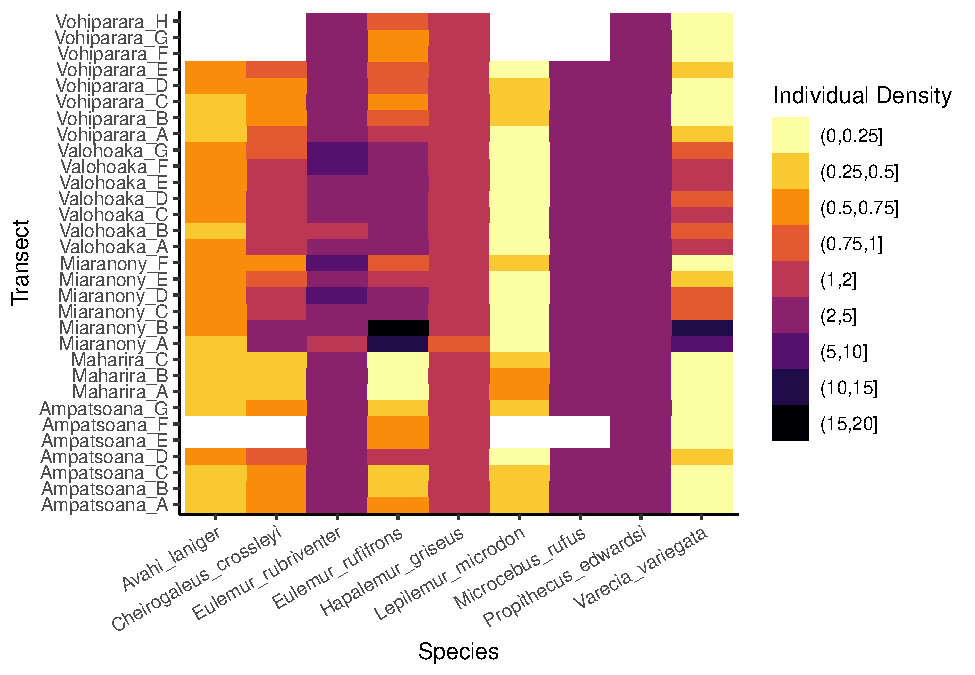
\includegraphics{project_draft_files/figure-latex/unnamed-chunk-1-1.pdf}
\caption{Figure 1. Heat map of lemur densities at each project transect
site}
\end{figure}

\begin{Shaded}
\begin{Highlighting}[]
\NormalTok{transect\_variables\_mean }\OtherTok{\textless{}{-}}\NormalTok{ lemur\_data }\SpecialCharTok{\%\textgreater{}\%}
  \FunctionTok{summarise}\NormalTok{(}\AttributeTok{LogFruitLength =} \FunctionTok{mean}\NormalTok{(logFruitLength),}
            \AttributeTok{LogFruitWidth =} \FunctionTok{mean}\NormalTok{(logFruitWidth),}
            \AttributeTok{LogSeedLength =} \FunctionTok{mean}\NormalTok{(logSeedLength),}
          \AttributeTok{LogSeedWidth =} \FunctionTok{mean}\NormalTok{(logSeedWidth),}
            \AttributeTok{LogSugar =} \FunctionTok{mean}\NormalTok{(logSugar),}
            \AttributeTok{LogFat =} \FunctionTok{mean}\NormalTok{(logFat),}
            \AttributeTok{LogProtein =} \FunctionTok{mean}\NormalTok{(logProtein),}
            \AttributeTok{LogNitrogen =} \FunctionTok{mean}\NormalTok{(logNitrogen),}
            \AttributeTok{LogTannins =} \FunctionTok{mean}\NormalTok{(logTannins),}
            \AttributeTok{SLA=} \FunctionTok{mean}\NormalTok{(logSLA),}
            \AttributeTok{WD=} \FunctionTok{mean}\NormalTok{(WD),}
            \AttributeTok{Tpi=} \FunctionTok{mean}\NormalTok{(tpi),}
            \AttributeTok{Roughness =} \FunctionTok{mean}\NormalTok{(roughness),}
            \AttributeTok{Slope =} \FunctionTok{mean}\NormalTok{(slope),}
            \AttributeTok{Aspect =} \FunctionTok{mean}\NormalTok{(aspect),}
            \AttributeTok{Flowdir =} \FunctionTok{mean}\NormalTok{(flowdir),}
          \AttributeTok{Density =} \FunctionTok{mean}\NormalTok{(Predicted)}
\NormalTok{            )}

\NormalTok{transect\_variables\_max }\OtherTok{\textless{}{-}}\NormalTok{ lemur\_data }\SpecialCharTok{\%\textgreater{}\%}
  \FunctionTok{summarise}\NormalTok{(}\AttributeTok{LogFruitLength =} \FunctionTok{max}\NormalTok{(logFruitLength),}
            \AttributeTok{LogFruitWidth =} \FunctionTok{max}\NormalTok{(logFruitWidth),}
            \AttributeTok{LogSeedLength =} \FunctionTok{max}\NormalTok{(logSeedLength),}
            \AttributeTok{LogSeedWidth =} \FunctionTok{max}\NormalTok{(logSeedWidth),}
            \AttributeTok{LogSugar =} \FunctionTok{max}\NormalTok{(logSugar),}
            \AttributeTok{LogFat =} \FunctionTok{max}\NormalTok{(logFat),}
            \AttributeTok{LogProtein =} \FunctionTok{max}\NormalTok{(logProtein),}
          \AttributeTok{LogNitrogen =} \FunctionTok{max}\NormalTok{(logNitrogen),}
            \AttributeTok{LogTannins =} \FunctionTok{max}\NormalTok{(logTannins),}
            \AttributeTok{SLA=} \FunctionTok{max}\NormalTok{(logSLA),}
            \AttributeTok{WD=} \FunctionTok{max}\NormalTok{(WD),}
            \AttributeTok{Tpi=}\FunctionTok{max}\NormalTok{(tpi),}
            \AttributeTok{Roughness =} \FunctionTok{max}\NormalTok{(roughness),}
            \AttributeTok{Slope =} \FunctionTok{max}\NormalTok{(slope),}
            \AttributeTok{Aspect =} \FunctionTok{max}\NormalTok{(aspect),}
            \AttributeTok{Flowdir =}\FunctionTok{max}\NormalTok{(flowdir),}
           \AttributeTok{Density =} \FunctionTok{max}\NormalTok{(Predicted)}
\NormalTok{            )}

\NormalTok{transect\_variables\_min }\OtherTok{\textless{}{-}}\NormalTok{ lemur\_data }\SpecialCharTok{\%\textgreater{}\%}
  \FunctionTok{summarise}\NormalTok{(}\AttributeTok{LogFruitLength =} \FunctionTok{min}\NormalTok{(logFruitLength),}
            \AttributeTok{LogFruitWidth =} \FunctionTok{min}\NormalTok{(logFruitWidth),}
            \AttributeTok{LogSeedLength =} \FunctionTok{min}\NormalTok{(logSeedLength),}
            \AttributeTok{LogSeedWidth =} \FunctionTok{min}\NormalTok{(logSeedWidth),}
          \AttributeTok{LogSugar =} \FunctionTok{min}\NormalTok{(logSugar),}
            \AttributeTok{LogFat =} \FunctionTok{min}\NormalTok{(logFat),}
            \AttributeTok{LogProtein =} \FunctionTok{min}\NormalTok{(logProtein),}
            \AttributeTok{LogNitrogen =} \FunctionTok{min}\NormalTok{(logNitrogen),}
            \AttributeTok{LogTannins =} \FunctionTok{min}\NormalTok{(logTannins),}
            \AttributeTok{SLA=} \FunctionTok{min}\NormalTok{(logSLA),}
            \AttributeTok{WD=} \FunctionTok{min}\NormalTok{(WD),}
            \AttributeTok{Tpi=}\FunctionTok{min}\NormalTok{(tpi),}
            \AttributeTok{Roughness =} \FunctionTok{min}\NormalTok{(roughness),}
            \AttributeTok{Slope =} \FunctionTok{min}\NormalTok{(slope),}
            \AttributeTok{Aspect =} \FunctionTok{min}\NormalTok{(aspect),}
            \AttributeTok{Flowdir =}\FunctionTok{min}\NormalTok{(flowdir),}
           \AttributeTok{Density =} \FunctionTok{min}\NormalTok{(Predicted)}
\NormalTok{            )}

\NormalTok{transect\_variables\_sd }\OtherTok{\textless{}{-}}\NormalTok{ lemur\_data }\SpecialCharTok{\%\textgreater{}\%}
  \FunctionTok{summarise}\NormalTok{(}\AttributeTok{LogFruitLength =} \FunctionTok{sd}\NormalTok{(logFruitLength),}
          \AttributeTok{LogFruitWidth =} \FunctionTok{sd}\NormalTok{(logFruitWidth),}
          \AttributeTok{LogSeedLength =} \FunctionTok{sd}\NormalTok{(logSeedLength),}
            \AttributeTok{LogSeedWidth =} \FunctionTok{sd}\NormalTok{(logSeedWidth),}
          \AttributeTok{LogSugar =} \FunctionTok{sd}\NormalTok{(logSugar),}
            \AttributeTok{LogFat =} \FunctionTok{sd}\NormalTok{(logFat),}
            \AttributeTok{LogProtein =} \FunctionTok{sd}\NormalTok{(logProtein),}
            \AttributeTok{LogNitrogen =} \FunctionTok{sd}\NormalTok{(logNitrogen),}
            \AttributeTok{LogTannins =} \FunctionTok{sd}\NormalTok{(logTannins),}
            \AttributeTok{SLA=} \FunctionTok{sd}\NormalTok{(logSLA),}
            \AttributeTok{WD=} \FunctionTok{sd}\NormalTok{(WD),}
            \AttributeTok{Tpi=}\FunctionTok{sd}\NormalTok{(tpi),}
            \AttributeTok{Roughness =} \FunctionTok{sd}\NormalTok{(roughness),}
            \AttributeTok{Slope =} \FunctionTok{sd}\NormalTok{(slope),}
            \AttributeTok{Aspect =} \FunctionTok{sd}\NormalTok{(aspect),}
            \AttributeTok{Flowdir =}\FunctionTok{sd}\NormalTok{(flowdir),}
           \AttributeTok{Density =} \FunctionTok{sd}\NormalTok{(Predicted)}
\NormalTok{            )}

\NormalTok{transect\_variables\_summary }\OtherTok{\textless{}{-}} \FunctionTok{rbind}\NormalTok{(transect\_variables\_max, transect\_variables\_min, transect\_variables\_mean, transect\_variables\_sd)}
\NormalTok{stats }\OtherTok{\textless{}{-}} \FunctionTok{c}\NormalTok{(}\StringTok{"Maximum"}\NormalTok{, }\StringTok{"Minimum"}\NormalTok{, }\StringTok{"Mean"}\NormalTok{, }\StringTok{"Standard Deviation"}\NormalTok{)}
\NormalTok{transect\_variables\_summary}\OtherTok{\textless{}{-}} \FunctionTok{cbind}\NormalTok{(stats, transect\_variables\_summary)}
\NormalTok{transect\_variables\_summary }\OtherTok{\textless{}{-}} \FunctionTok{data.frame}\NormalTok{(}\FunctionTok{t}\NormalTok{(transect\_variables\_summary[}\SpecialCharTok{{-}}\DecValTok{1}\NormalTok{]))}
\FunctionTok{colnames}\NormalTok{(transect\_variables\_summary) }\OtherTok{\textless{}{-}} \FunctionTok{c}\NormalTok{(}\StringTok{"Maximum"}\NormalTok{, }\StringTok{"Minimum"}\NormalTok{, }\StringTok{"Mean"}\NormalTok{, }\StringTok{"Standard Deviation"}\NormalTok{)}

\FunctionTok{kable}\NormalTok{(transect\_variables\_summary, }\AttributeTok{caption =}\StringTok{"Table 1. Summary Statistics for Transect{-}Level Variables"}\NormalTok{)}
\end{Highlighting}
\end{Shaded}

\begin{longtable}[]{@{}lrrrr@{}}
\caption{Table 1. Summary Statistics for Transect-Level
Variables}\tabularnewline
\toprule
& Maximum & Minimum & Mean & Standard Deviation\tabularnewline
\midrule
\endfirsthead
\toprule
& Maximum & Minimum & Mean & Standard Deviation\tabularnewline
\midrule
\endhead
LogFruitLength & 3.0367699 & 2.5481124 & 2.7884419 &
0.1078722\tabularnewline
LogFruitWidth & 2.8735245 & 2.4061911 & 2.6418949 &
0.1105788\tabularnewline
LogSeedLength & 2.4618778 & 1.8435241 & 2.2224035 &
0.1463275\tabularnewline
LogSeedWidth & 2.1370075 & 1.5738239 & 1.9532329 &
0.1329052\tabularnewline
LogSugar & 2.6292634 & 2.0849150 & 2.3969571 & 0.1121973\tabularnewline
LogFat & 1.8455284 & 1.5255786 & 1.6830810 & 0.0767810\tabularnewline
LogProtein & 4.2689341 & 3.2368227 & 3.7342967 &
0.2510554\tabularnewline
LogNitrogen & 0.9160242 & 0.7243437 & 0.8042614 &
0.0578926\tabularnewline
LogTannins & 0.1913672 & 0.0687408 & 0.1419214 &
0.0294709\tabularnewline
SLA & 2.4679473 & 2.2134377 & 2.3677036 & 0.0578060\tabularnewline
WD & 0.5986437 & 0.5414205 & 0.5804747 & 0.0101335\tabularnewline
Tpi & 73.7500000 & -206.7500000 & -0.3527992 & 60.5243149\tabularnewline
Roughness & 529.0000000 & 34.0000000 & 205.0308880 &
151.3989769\tabularnewline
Slope & 13.5005877 & 0.3904947 & 4.2638428 & 3.6935512\tabularnewline
Aspect & 280.1872004 & 9.7805570 & 135.9507256 &
67.2499763\tabularnewline
Flowdir & 64.0000000 & 1.0000000 & 6.2355212 & 10.1291339\tabularnewline
Density & 17.9717477 & 0.0566592 & 1.7848451 & 2.0068795\tabularnewline
\bottomrule
\end{longtable}

\newpage

\hypertarget{analysis}{%
\section{Analysis}\label{analysis}}

\textless\textless\textless\textless\textless\textless\textless{} HEAD
\#\# Question 1: Are there significant differences in lemur densities
among the different sites and among the different species? If so, how
can the sites and species be grouped to reflect the patterns in
densities? =======

First, we conducted a one-way analysis of variance (ANOVA) on lemur
population density by site using the ``aov'' function in the R general
interface. Next, we completed a post-hoc Tukey HSD test to determine
pairwise differences between the sites. Then, we conducted a HSD
post-hoc test from the R package ``agricolae'' (de Mendiburu 2020) to
categorize the sites into groups based on their lemur densities. After
these analyses of the sites, we repeated the process between lemur
species rather than sites to determine if there are significant
differences in densities depending on the particular species.
Visualizations were conducted using the ``ggplot2'' package (Wockham
2016).

\begin{Shaded}
\begin{Highlighting}[]
\NormalTok{trait\_data2 }\OtherTok{\textless{}{-}}\NormalTok{ lemur\_data }\SpecialCharTok{\%\textgreater{}\%}
  \FunctionTok{mutate}\NormalTok{(}\AttributeTok{Transect\_Site2 =}\NormalTok{ Transect\_Site)}\SpecialCharTok{\%\textgreater{}\%}
  \FunctionTok{separate}\NormalTok{(}\AttributeTok{col=}\NormalTok{ Transect\_Site2, }\AttributeTok{into=}\StringTok{"Site"}\NormalTok{, }\AttributeTok{sep =}\StringTok{"\_"}\NormalTok{)}
\end{Highlighting}
\end{Shaded}

\begin{verbatim}
## Warning: Expected 1 pieces. Additional pieces discarded in 259 rows [1, 2, 3, 4,
## 5, 6, 7, 8, 9, 10, 11, 12, 13, 14, 15, 16, 17, 18, 19, 20, ...].
\end{verbatim}

\begin{Shaded}
\begin{Highlighting}[]
\CommentTok{\#write.csv(trait\_data2, "C:/ENV872/LemurProject\_DeSisto\_Gonzalez\_Horn/Data/Processed/trait\_data2.csv")}


\NormalTok{density\_anova }\OtherTok{\textless{}{-}} \FunctionTok{aov}\NormalTok{(}\AttributeTok{data=}\NormalTok{ trait\_data2, Predicted }\SpecialCharTok{\textasciitilde{}}\NormalTok{ Site)}
\FunctionTok{summary}\NormalTok{(density\_anova)}
\end{Highlighting}
\end{Shaded}

\begin{verbatim}
##              Df Sum Sq Mean Sq F value  Pr(>F)   
## Site          4   53.8  13.455   3.469 0.00884 **
## Residuals   254  985.3   3.879                   
## ---
## Signif. codes:  0 '***' 0.001 '**' 0.01 '*' 0.05 '.' 0.1 ' ' 1
\end{verbatim}

\begin{Shaded}
\begin{Highlighting}[]
\CommentTok{\#I reject the null hypothesis and conclude that there is a significant difference in lemur densities between different sites (p = 0.009). }
\FunctionTok{TukeyHSD}\NormalTok{(density\_anova)}
\end{Highlighting}
\end{Shaded}

\begin{verbatim}
##   Tukey multiple comparisons of means
##     95% family-wise confidence level
## 
## Fit: aov(formula = Predicted ~ Site, data = trait_data2)
## 
## $Site
##                              diff         lwr         upr     p adj
## Maharira-Ampatsoana   -0.24434525 -1.51592352  1.02723302 0.9844326
## Miaranony-Ampatsoana   1.11175034  0.07509492  2.14840576 0.0287003
## Valohoaka-Ampatsoana   0.49076493 -0.50782868  1.48935854 0.6599856
## Vohiparara-Ampatsoana  0.06169045 -0.94847230  1.07185319 0.9998214
## Miaranony-Maharira     1.35609559  0.08064645  2.63154473 0.0308715
## Valohoaka-Maharira     0.73511018 -0.50960073  1.97982109 0.4843107
## Vohiparara-Maharira    0.30603570 -0.94797580  1.56004719 0.9625640
## Valohoaka-Miaranony   -0.62098541 -1.62450343  0.38253261 0.4356786
## Vohiparara-Miaranony  -1.05005989 -2.06509092 -0.03502886 0.0385856
## Vohiparara-Valohoaka  -0.42907448 -1.40520087  0.54705191 0.7469374
\end{verbatim}

\begin{Shaded}
\begin{Highlighting}[]
\CommentTok{\# There is a significant difference in lemur densities between Miaranony and Ampatsoana, Miaranony and Maharira, }
\CommentTok{\#and Miaranony and Vohiparara }

\NormalTok{anova\_groups }\OtherTok{\textless{}{-}} \FunctionTok{HSD.test}\NormalTok{(density\_anova, }\StringTok{"Site"}\NormalTok{, }\AttributeTok{group=}\ConstantTok{TRUE}\NormalTok{)}
\CommentTok{\# the predicted groups according to their lemur densities are Miaranony and Valohoaka being in group a }
\CommentTok{\# and Valohoaka, Vohiparara, Ampatsoana, and Maharira in group b }


\NormalTok{density\_aov\_plot }\OtherTok{\textless{}{-}} \FunctionTok{ggplot}\NormalTok{(}\AttributeTok{data =}\NormalTok{ trait\_data2, }\FunctionTok{aes}\NormalTok{(}\AttributeTok{x =}\NormalTok{ Site, }\AttributeTok{y =}\NormalTok{ Predicted))}\SpecialCharTok{+}
  \FunctionTok{geom\_boxplot}\NormalTok{()}\SpecialCharTok{+}
  \FunctionTok{ylab}\NormalTok{(}\StringTok{"Lemur Density (N Individuals/"}\SpecialCharTok{\textasciitilde{}}\NormalTok{(Km}\SpecialCharTok{\^{}}\DecValTok{2}\NormalTok{))}\SpecialCharTok{+}
  \FunctionTok{theme\_classic}\NormalTok{()}
\CommentTok{\#based on the plot it looks like it might be outliers that are driving the pattern we see of higher lemur densities}
\CommentTok{\# in Miaranony and Valohoaka}
\end{Highlighting}
\end{Shaded}

\begin{Shaded}
\begin{Highlighting}[]
\NormalTok{density\_anova2 }\OtherTok{\textless{}{-}} \FunctionTok{aov}\NormalTok{(}\AttributeTok{data=}\NormalTok{ trait\_data2, Predicted }\SpecialCharTok{\textasciitilde{}}\NormalTok{ Species)}
\FunctionTok{summary}\NormalTok{(density\_anova2)}
\end{Highlighting}
\end{Shaded}

\begin{verbatim}
##              Df Sum Sq Mean Sq F value Pr(>F)    
## Species       8  363.2    45.4   16.79 <2e-16 ***
## Residuals   250  675.9     2.7                   
## ---
## Signif. codes:  0 '***' 0.001 '**' 0.01 '*' 0.05 '.' 0.1 ' ' 1
\end{verbatim}

\begin{Shaded}
\begin{Highlighting}[]
\CommentTok{\#I reject the null hypothesis and conclude that there is a significant difference in lemur densities between different species (p \textless{} 0.001).}

\FunctionTok{TukeyHSD}\NormalTok{(density\_anova2)}
\end{Highlighting}
\end{Shaded}

\begin{verbatim}
##   Tukey multiple comparisons of means
##     95% family-wise confidence level
## 
## Fit: aov(formula = Predicted ~ Species, data = trait_data2)
## 
## $Species
##                                                    diff         lwr
## Cheirogaleus_crossleyi-Avahi_laniger         0.41233752 -1.01469480
## Eulemur_rubriventer-Avahi_laniger            3.30306813  1.93478684
## Eulemur_rufifrons-Avahi_laniger              1.81868377  0.45040247
## Hapalemur_griseus-Avahi_laniger              0.62028125 -0.74800004
## Lepilemur_microdon-Avahi_laniger            -0.25848688 -1.68551919
## Microcebus_rufus-Avahi_laniger               2.22014703  0.79311471
## Propithecus_edwardsi-Avahi_laniger           2.53047986  1.16219857
## Varecia_variegata-Avahi_laniger              0.50347344 -0.86480786
## Eulemur_rubriventer-Cheirogaleus_crossleyi   2.89073061  1.52244932
## Eulemur_rufifrons-Cheirogaleus_crossleyi     1.40634625  0.03806496
## Hapalemur_griseus-Cheirogaleus_crossleyi     0.20794373 -1.16033756
## Lepilemur_microdon-Cheirogaleus_crossleyi   -0.67082440 -2.09785671
## Microcebus_rufus-Cheirogaleus_crossleyi      1.80780951  0.38077720
## Propithecus_edwardsi-Cheirogaleus_crossleyi  2.11814235  0.74986105
## Varecia_variegata-Cheirogaleus_crossleyi     0.09113592 -1.27714537
## Eulemur_rufifrons-Eulemur_rubriventer       -1.48438436 -2.79127617
## Hapalemur_griseus-Eulemur_rubriventer       -2.68278688 -3.98967868
## Lepilemur_microdon-Eulemur_rubriventer      -3.56155501 -4.92983631
## Microcebus_rufus-Eulemur_rubriventer        -1.08292111 -2.45120240
## Propithecus_edwardsi-Eulemur_rubriventer    -0.77258827 -2.07948007
## Varecia_variegata-Eulemur_rubriventer       -2.79959469 -4.10648650
## Hapalemur_griseus-Eulemur_rufifrons         -1.19840252 -2.50529432
## Lepilemur_microdon-Eulemur_rufifrons        -2.07717065 -3.44545194
## Microcebus_rufus-Eulemur_rufifrons           0.40146326 -0.96681804
## Propithecus_edwardsi-Eulemur_rufifrons       0.71179610 -0.59509571
## Varecia_variegata-Eulemur_rufifrons         -1.31521033 -2.62210213
## Lepilemur_microdon-Hapalemur_griseus        -0.87876813 -2.24704943
## Microcebus_rufus-Hapalemur_griseus           1.59986577  0.23158448
## Propithecus_edwardsi-Hapalemur_griseus       1.91019861  0.60330681
## Varecia_variegata-Hapalemur_griseus         -0.11680781 -1.42369962
## Microcebus_rufus-Lepilemur_microdon          2.47863390  1.05160159
## Propithecus_edwardsi-Lepilemur_microdon      2.78896674  1.42068545
## Varecia_variegata-Lepilemur_microdon         0.76196032 -0.60632098
## Propithecus_edwardsi-Microcebus_rufus        0.31033284 -1.05794846
## Varecia_variegata-Microcebus_rufus          -1.71667359 -3.08495488
## Varecia_variegata-Propithecus_edwardsi      -2.02700643 -3.33389823
##                                                      upr     p adj
## Cheirogaleus_crossleyi-Avahi_laniger         1.839369830 0.9925947
## Eulemur_rubriventer-Avahi_laniger            4.671349428 0.0000000
## Eulemur_rufifrons-Avahi_laniger              3.186965064 0.0014338
## Hapalemur_griseus-Avahi_laniger              1.988562546 0.8898724
## Lepilemur_microdon-Avahi_laniger             1.168545434 0.9997365
## Microcebus_rufus-Avahi_laniger               3.647179338 0.0000692
## Propithecus_edwardsi-Avahi_laniger           3.898761160 0.0000008
## Varecia_variegata-Avahi_laniger              1.871754734 0.9654778
## Eulemur_rubriventer-Cheirogaleus_crossleyi   4.259011910 0.0000000
## Eulemur_rufifrons-Cheirogaleus_crossleyi     2.774627546 0.0387346
## Hapalemur_griseus-Cheirogaleus_crossleyi     1.576225029 0.9999300
## Lepilemur_microdon-Cheirogaleus_crossleyi    0.756207916 0.8679449
## Microcebus_rufus-Cheirogaleus_crossleyi      3.234841821 0.0030530
## Propithecus_edwardsi-Cheirogaleus_crossleyi  3.486423642 0.0000773
## Varecia_variegata-Cheirogaleus_crossleyi     1.459417217 0.9999999
## Eulemur_rufifrons-Eulemur_rubriventer       -0.177492560 0.0132340
## Hapalemur_griseus-Eulemur_rubriventer       -1.375895078 0.0000000
## Lepilemur_microdon-Eulemur_rubriventer      -2.193273716 0.0000000
## Microcebus_rufus-Eulemur_rubriventer         0.285360189 0.2485246
## Propithecus_edwardsi-Eulemur_rubriventer     0.534303535 0.6487500
## Varecia_variegata-Eulemur_rubriventer       -1.492702890 0.0000000
## Hapalemur_griseus-Eulemur_rufifrons          0.108489286 0.1013056
## Lepilemur_microdon-Eulemur_rufifrons        -0.708889352 0.0001180
## Microcebus_rufus-Eulemur_rufifrons           1.769744553 0.9917960
## Propithecus_edwardsi-Eulemur_rufifrons       2.018687899 0.7434653
## Varecia_variegata-Eulemur_rufifrons         -0.008318526 0.0472010
## Lepilemur_microdon-Hapalemur_griseus         0.489513165 0.5380854
## Microcebus_rufus-Hapalemur_griseus           2.968147070 0.0092519
## Propithecus_edwardsi-Hapalemur_griseus       3.217090417 0.0002567
## Varecia_variegata-Hapalemur_griseus          1.190083991 0.9999989
## Microcebus_rufus-Lepilemur_microdon          3.905666217 0.0000046
## Propithecus_edwardsi-Lepilemur_microdon      4.157248039 0.0000000
## Varecia_variegata-Lepilemur_microdon         2.130241614 0.7195202
## Propithecus_edwardsi-Microcebus_rufus        1.678614134 0.9986281
## Varecia_variegata-Microcebus_rufus          -0.348392291 0.0035252
## Varecia_variegata-Propithecus_edwardsi      -0.720114622 0.0000741
\end{verbatim}

\begin{Shaded}
\begin{Highlighting}[]
\NormalTok{anova\_groups2 }\OtherTok{\textless{}{-}} \FunctionTok{HSD.test}\NormalTok{(density\_anova2, }\StringTok{"Species"}\NormalTok{, }\AttributeTok{group=}\ConstantTok{TRUE}\NormalTok{)}
\CommentTok{\# the lemur species fall into four groups according to their densities }
\CommentTok{\#What is interesting is that the groups do not seem to be organized by taxonomic family, body size, or whether they are nocturnal. diurnal}

\NormalTok{density\_aov\_plot2 }\OtherTok{\textless{}{-}} \FunctionTok{ggplot}\NormalTok{(}\AttributeTok{data =}\NormalTok{ trait\_data2, }\FunctionTok{aes}\NormalTok{(}\AttributeTok{x =} \FunctionTok{reorder}\NormalTok{(Species, Predicted, }\AttributeTok{FUN =}\NormalTok{ median), }\AttributeTok{y =}\NormalTok{ Predicted))}\SpecialCharTok{+}
  \FunctionTok{geom\_boxplot}\NormalTok{()}\SpecialCharTok{+}
  \FunctionTok{ylab}\NormalTok{(}\StringTok{"Lemur Density (N Individuals/"}\SpecialCharTok{\textasciitilde{}}\NormalTok{(Km}\SpecialCharTok{\^{}}\DecValTok{2}\NormalTok{))}\SpecialCharTok{+}
  \FunctionTok{xlab}\NormalTok{(}\StringTok{"Species"}\NormalTok{)}\SpecialCharTok{+}
  \FunctionTok{theme\_classic}\NormalTok{()}\SpecialCharTok{+}
  \FunctionTok{scale\_x\_discrete}\NormalTok{(}\AttributeTok{labels=} \FunctionTok{c}\NormalTok{(}\StringTok{"V. variegata"}\NormalTok{, }\StringTok{"L. microdon"}\NormalTok{, }\StringTok{"A. laniger"}\NormalTok{, }\StringTok{"C. crossleyi"}\NormalTok{, }\StringTok{"E. rufifrons"}\NormalTok{, }\StringTok{"H. gruseus"}\NormalTok{, }\StringTok{"M. rufus"}\NormalTok{, }\StringTok{"P. edwardsi"}\NormalTok{, }\StringTok{"E. rubriventer"}\NormalTok{))}\SpecialCharTok{+}
  \FunctionTok{theme}\NormalTok{(}\AttributeTok{axis.text.x =} \FunctionTok{element\_text}\NormalTok{(}\AttributeTok{angle =} \DecValTok{45}\NormalTok{, }\AttributeTok{vjust=}\FloatTok{0.5}\NormalTok{))}
\end{Highlighting}
\end{Shaded}

\hypertarget{question-2-what-variables-are-related-to-differences-in-lemur-densities}{%
\subsection{Question 2: What variables are related to differences in
lemur
densities?}\label{question-2-what-variables-are-related-to-differences-in-lemur-densities}}

Next, weanalyzed what transect-level habitat variables are significantly
related to lemur densities. After an exploratory correlation plot to
determine the correlations between the habitat variables, we conducted
linear mixed effects models using the ``lmer'' function in the R package
``lme4'' (Bates et al.~2015). We used lemur density as the dependent
variable, site-level habitat characteristics (log fruit length, log
fruit width, log seed length, log seed width, log fruit nitrogen
content, log tree tannin content, log fruit sugar content, log fruit
sugar content, log fruit protein content, latitude, longitude, aspect,
slope, and roughness) as the independent variables. We conducted these
models with both the transect and the lemur species as random variables.
In the first set of models we included site as an independent variable,
and in a second set of models we included it as a random variable. We
used a backward stepwise approach to reduce the models and conducted
model selection via comparison of their Akaike Information Criterion
(AIC) values using the ``lrtest'' function in the R package ``lmtest''
(Zeileis \& Horton 2002). Additionally, we identified the R-squared
values of the models using the ``r.squaredGLMM'' function in the R
package ``MuMln'' (Barton 2020).

\hypertarget{question-3-which-landscape-level-characteristics-and-plant-functional-traits-influence-density-of-individual-lemur-species}{%
\subsection{Question 3: Which landscape-level characteristics and plant
functional traits influence density of individual lemur
species?}\label{question-3-which-landscape-level-characteristics-and-plant-functional-traits-influence-density-of-individual-lemur-species}}

The final step of our analyses was exploring the effects of habitat
variables for specific lemur species. To do this, we subset the data by
species and conducted linear models for four lemur species (\emph{Avahi
laniger, Eulemur rubriventer, Propithecus edwardsi}, and \emph{Lepilemur
microdon}) using the function ``lm'' from the R general interface. We
used density as the dependent variable and the aforementioned habitat
variables as independent variables. We chose to focus on these four
lemur species as case studies because we identified them as having
distinct densities based on the ANOVA and exploratory data analysis.
Further, we identified \emph{Avahi laniger} and \emph{Lepilemur
microdon} as having the two lowest mean densities of all species
included in our data, and we identified \emph{Propithecus edwardsi} and
\emph{Eulemur rubriventer} as having the two highest mean densities of
all species included in our data. Therefore, analyzing these four
species individually could provide us with insights into drivers of high
and low densities.

\begin{Shaded}
\begin{Highlighting}[]
\CommentTok{\#More analyses using linear models}
\NormalTok{traitdata\_subset }\OtherTok{\textless{}{-}} \FunctionTok{select}\NormalTok{(trait\_data2, logFruitLength}\SpecialCharTok{:}\NormalTok{logSLA, Predicted, slope, aspect, lat, long)}
\NormalTok{lemur\_density\_Corr }\OtherTok{\textless{}{-}} \FunctionTok{cor}\NormalTok{(traitdata\_subset)}
\FunctionTok{corrplot}\NormalTok{(lemur\_density\_Corr, }\AttributeTok{method =} \StringTok{"ellipse"}\NormalTok{)}
\end{Highlighting}
\end{Shaded}

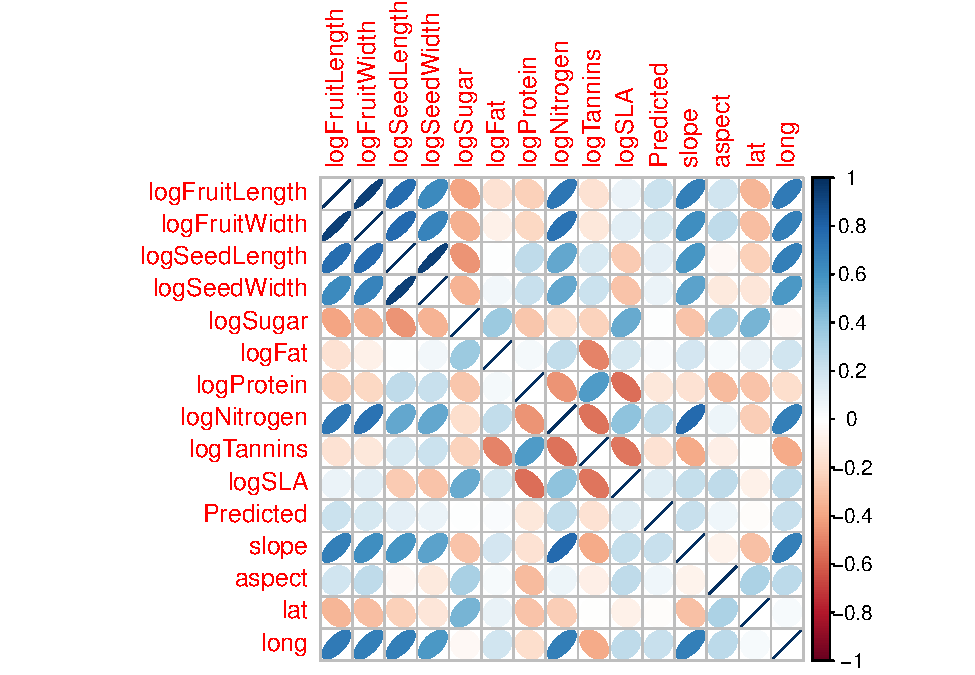
\includegraphics{project_draft_files/figure-latex/unnamed-chunk-5-1.pdf}

\begin{Shaded}
\begin{Highlighting}[]
\CommentTok{\#The correlation plot matrix indicates that there are slight correlations between our response variable (Predicted) and multiple explanatory variables.}


\NormalTok{Fruit\_trait\_plot }\OtherTok{\textless{}{-}} \FunctionTok{ggplot}\NormalTok{(traitdata\_subset, }\FunctionTok{aes}\NormalTok{(}\AttributeTok{x =}\NormalTok{ logFruitLength, }\AttributeTok{y =}\NormalTok{ Predicted, }\AttributeTok{color =}\NormalTok{ logNitrogen)) }\SpecialCharTok{+}
  \FunctionTok{geom\_point}\NormalTok{()}
\FunctionTok{print}\NormalTok{(Fruit\_trait\_plot)}
\end{Highlighting}
\end{Shaded}

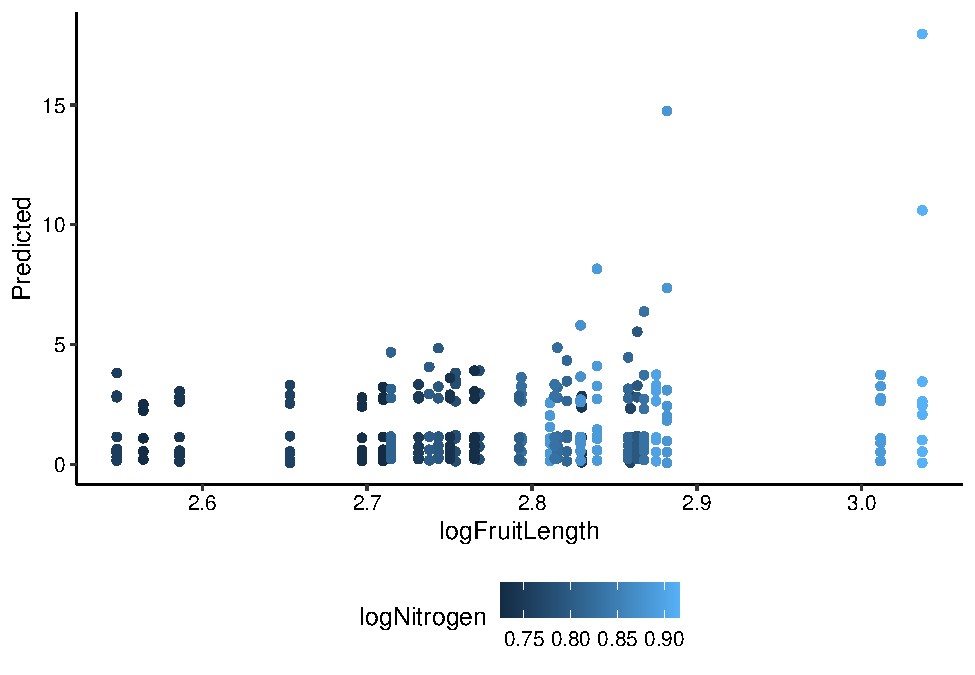
\includegraphics{project_draft_files/figure-latex/unnamed-chunk-5-2.pdf}

\begin{Shaded}
\begin{Highlighting}[]
\CommentTok{\# plot to visually explore the relationship between some of fruit trait variables that stood out in the correlation plot matrix and lemur density}

\NormalTok{Fruit\_trait\_nutrient\_plot2 }\OtherTok{\textless{}{-}} \FunctionTok{ggplot}\NormalTok{(traitdata\_subset, }\FunctionTok{aes}\NormalTok{(}\AttributeTok{x =}\NormalTok{ logProtein, }\AttributeTok{y =}\NormalTok{ Predicted, }\AttributeTok{color =}\NormalTok{ logTannins)) }\SpecialCharTok{+}
  \FunctionTok{geom\_point}\NormalTok{()}
\FunctionTok{print}\NormalTok{(Fruit\_trait\_nutrient\_plot2)}
\end{Highlighting}
\end{Shaded}

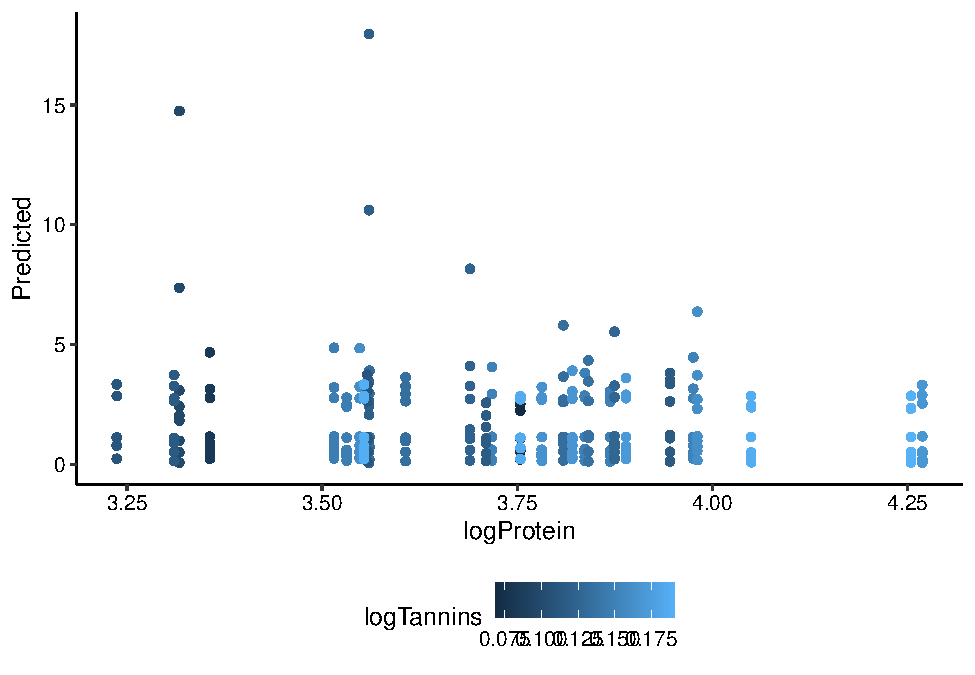
\includegraphics{project_draft_files/figure-latex/unnamed-chunk-5-3.pdf}

\begin{Shaded}
\begin{Highlighting}[]
\CommentTok{\# plot to visually explore the relationship between two other fruit trait variables that stood out in the correlation plot matrix and lemur density}

\CommentTok{\#Creating a linear model with random effects (transect site and species as random effects)}
\NormalTok{lemur\_dens\_lmer1 }\OtherTok{\textless{}{-}} \FunctionTok{lmer}\NormalTok{(}\AttributeTok{data =}\NormalTok{ trait\_data2, Predicted }\SpecialCharTok{\textasciitilde{}}\NormalTok{ logSeedLength }\SpecialCharTok{+}\NormalTok{ logNitrogen }\SpecialCharTok{+}\NormalTok{ lat }\SpecialCharTok{+}\NormalTok{ logSeedWidth }\SpecialCharTok{+}\NormalTok{ logTannins }\SpecialCharTok{+}\NormalTok{ roughness }\SpecialCharTok{+}\NormalTok{ long }\SpecialCharTok{+}\NormalTok{ logSugar }\SpecialCharTok{+}\NormalTok{ logSLA }\SpecialCharTok{+}\NormalTok{ slope }\SpecialCharTok{+}\NormalTok{Site}\SpecialCharTok{+}\NormalTok{ logFruitLength }\SpecialCharTok{+}\NormalTok{ logFat }\SpecialCharTok{+}\NormalTok{ aspect }\SpecialCharTok{+}\NormalTok{ logFruitWidth }\SpecialCharTok{+}\NormalTok{ logProtein }\SpecialCharTok{+}\NormalTok{ (}\DecValTok{1}\SpecialCharTok{|}\NormalTok{Species) }\SpecialCharTok{+}\NormalTok{ (}\DecValTok{1}\SpecialCharTok{|}\NormalTok{Transect\_Site))}
\end{Highlighting}
\end{Shaded}

\begin{verbatim}
## Warning: Some predictor variables are on very different scales: consider
## rescaling
\end{verbatim}

\begin{verbatim}
## boundary (singular) fit: see ?isSingular
\end{verbatim}

\begin{verbatim}
## Warning: Some predictor variables are on very different scales: consider
## rescaling
\end{verbatim}

\begin{Shaded}
\begin{Highlighting}[]
\FunctionTok{summary}\NormalTok{(lemur\_dens\_lmer1)}
\end{Highlighting}
\end{Shaded}

\begin{verbatim}
## Linear mixed model fit by REML. t-tests use Satterthwaite's method [
## lmerModLmerTest]
## Formula: Predicted ~ logSeedLength + logNitrogen + lat + logSeedWidth +  
##     logTannins + roughness + long + logSugar + logSLA + slope +  
##     Site + logFruitLength + logFat + aspect + logFruitWidth +  
##     logProtein + (1 | Species) + (1 | Transect_Site)
##    Data: trait_data2
## 
## REML criterion at convergence: 942.2
## 
## Scaled residuals: 
##     Min      1Q  Median      3Q     Max 
## -2.4001 -0.2993 -0.0091  0.2590  8.5591 
## 
## Random effects:
##  Groups        Name        Variance  Std.Dev. 
##  Transect_Site (Intercept) 1.125e-11 3.354e-06
##  Species       (Intercept) 1.563e+00 1.250e+00
##  Residual                  2.374e+00 1.541e+00
## Number of obs: 259, groups:  Transect_Site, 31; Species, 9
## 
## Fixed effects:
##                  Estimate Std. Error         df t value Pr(>|t|)   
## (Intercept)    -18.771085 616.337417 230.883243  -0.030  0.97573   
## logSeedLength    0.564743   4.280281 231.037733   0.132  0.89515   
## logNitrogen     15.507459   5.807085 230.997034   2.670  0.00811 **
## lat            -25.853124  12.960069 231.092886  -1.995  0.04724 * 
## logSeedWidth    -2.666833   4.783737 231.003118  -0.557  0.57774   
## logTannins       5.047217  10.863562 231.085231   0.465  0.64265   
## roughness       -0.006877   0.003449 230.994197  -1.994  0.04733 * 
## long           -11.359045  13.294831 230.946483  -0.854  0.39377   
## logSugar         2.601340   2.692910 230.997313   0.966  0.33506   
## logSLA           0.162660   4.549210 231.028321   0.036  0.97151   
## slope            0.239327   0.136268 230.991674   1.756  0.08036 . 
## SiteMaharira    -7.968357   4.513314 231.058902  -1.766  0.07880 . 
## SiteMiaranony   -1.419236   2.010303 230.942810  -0.706  0.48091   
## SiteValohoaka   -7.237059   3.725982 231.041098  -1.942  0.05331 . 
## SiteVohiparara  -6.154208   2.893724 231.079496  -2.127  0.03450 * 
## logFruitLength   8.252693   4.542446 230.992059   1.817  0.07054 . 
## logFat          -1.431096   2.397225 231.044363  -0.597  0.55111   
## aspect          -0.001160   0.002815 230.997184  -0.412  0.68067   
## logFruitWidth   -8.690045   4.130924 231.002929  -2.104  0.03649 * 
## logProtein       0.764685   1.130087 231.013454   0.677  0.49930   
## ---
## Signif. codes:  0 '***' 0.001 '**' 0.01 '*' 0.05 '.' 0.1 ' ' 1
\end{verbatim}

\begin{verbatim}
## 
## Correlation matrix not shown by default, as p = 20 > 12.
## Use print(x, correlation=TRUE)  or
##     vcov(x)        if you need it
\end{verbatim}

\begin{verbatim}
## fit warnings:
## Some predictor variables are on very different scales: consider rescaling
## optimizer (nloptwrap) convergence code: 0 (OK)
## boundary (singular) fit: see ?isSingular
\end{verbatim}

\begin{Shaded}
\begin{Highlighting}[]
\CommentTok{\#Checking whether the linear model conforms to the assumptions of linear models}
\FunctionTok{par}\NormalTok{(}\AttributeTok{mfrow =} \FunctionTok{c}\NormalTok{(}\DecValTok{2}\NormalTok{,}\DecValTok{2}\NormalTok{), }\AttributeTok{mar=}\FunctionTok{c}\NormalTok{(}\DecValTok{4}\NormalTok{,}\DecValTok{4}\NormalTok{,}\DecValTok{4}\NormalTok{,}\DecValTok{4}\NormalTok{))}
\FunctionTok{plot}\NormalTok{(lemur\_dens\_lmer1)}
\end{Highlighting}
\end{Shaded}

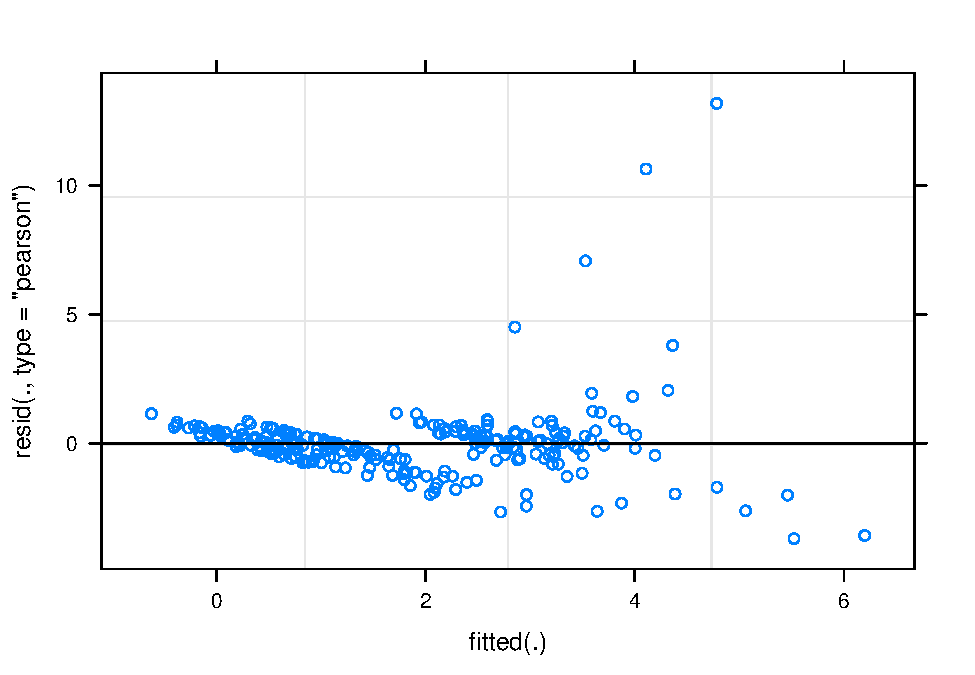
\includegraphics{project_draft_files/figure-latex/unnamed-chunk-5-4.pdf}

\begin{Shaded}
\begin{Highlighting}[]
\FunctionTok{par}\NormalTok{(}\AttributeTok{mfrow =} \FunctionTok{c}\NormalTok{(}\DecValTok{1}\NormalTok{,}\DecValTok{1}\NormalTok{))}
\CommentTok{\#There appears to be a balance of positive and negative residuals, which is a good sign. However, there appears to be a strange pattern of three separate lines with negative slopes}

\FunctionTok{qqnorm}\NormalTok{(trait\_data2}\SpecialCharTok{$}\NormalTok{Predicted); }\FunctionTok{qqline}\NormalTok{(trait\_data2}\SpecialCharTok{$}\NormalTok{Predicted)}
\end{Highlighting}
\end{Shaded}

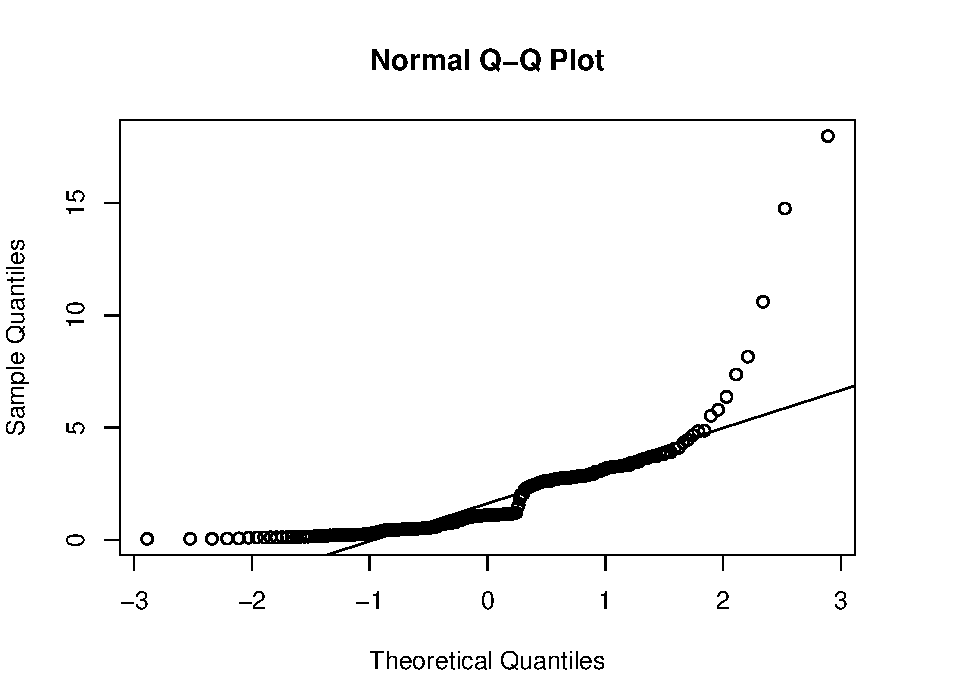
\includegraphics{project_draft_files/figure-latex/unnamed-chunk-5-5.pdf}

\begin{Shaded}
\begin{Highlighting}[]
\CommentTok{\#This qqplot provides information on the normality of the response variable. The data doesn\textquotesingle{}t follow a normal distribution that well, but I don\textquotesingle{}t think its terrible}


\CommentTok{\#Reducing the linear model manually}
\NormalTok{lemur\_dens\_lmer2 }\OtherTok{\textless{}{-}} \FunctionTok{update}\NormalTok{(lemur\_dens\_lmer1,}\SpecialCharTok{\textasciitilde{}}\NormalTok{.}\SpecialCharTok{{-}}\NormalTok{logSLA)}
\end{Highlighting}
\end{Shaded}

\begin{verbatim}
## Warning: Some predictor variables are on very different scales: consider
## rescaling
\end{verbatim}

\begin{verbatim}
## boundary (singular) fit: see ?isSingular
\end{verbatim}

\begin{verbatim}
## Warning: Some predictor variables are on very different scales: consider
## rescaling
\end{verbatim}

\begin{Shaded}
\begin{Highlighting}[]
\FunctionTok{summary}\NormalTok{(lemur\_dens\_lmer2)}
\end{Highlighting}
\end{Shaded}

\begin{verbatim}
## Linear mixed model fit by REML. t-tests use Satterthwaite's method [
## lmerModLmerTest]
## Formula: Predicted ~ logSeedLength + logNitrogen + lat + logSeedWidth +  
##     logTannins + roughness + long + logSugar + slope + Site +  
##     logFruitLength + logFat + aspect + logFruitWidth + logProtein +  
##     (1 | Species) + (1 | Transect_Site)
##    Data: trait_data2
## 
## REML criterion at convergence: 947
## 
## Scaled residuals: 
##     Min      1Q  Median      3Q     Max 
## -2.4045 -0.2986 -0.0093  0.2604  8.5760 
## 
## Random effects:
##  Groups        Name        Variance  Std.Dev. 
##  Transect_Site (Intercept) 1.945e-10 1.395e-05
##  Species       (Intercept) 1.563e+00 1.250e+00
##  Residual                  2.364e+00 1.537e+00
## Number of obs: 259, groups:  Transect_Site, 31; Species, 9
## 
## Fixed effects:
##                  Estimate Std. Error         df t value Pr(>|t|)   
## (Intercept)    -26.674315 573.799178 232.157724  -0.046  0.96296   
## logSeedLength    0.546642   4.241875 232.036918   0.129  0.89757   
## logNitrogen     15.571900   5.508461 232.014680   2.827  0.00511 **
## lat            -25.771740  12.724015 232.110126  -2.025  0.04397 * 
## logSeedWidth    -2.683522   4.750223 232.007443  -0.565  0.57267   
## logTannins       5.113201  10.686930 232.084293   0.478  0.63278   
## roughness       -0.006896   0.003400 232.000108  -2.028  0.04369 * 
## long           -11.148195  11.873011 232.230010  -0.939  0.34873   
## logSugar         2.653271   2.260511 232.043294   1.174  0.24170   
## slope            0.240850   0.129138 232.002284   1.865  0.06344 . 
## SiteMaharira    -7.924850   4.333427 232.084895  -1.829  0.06872 . 
## SiteMiaranony   -1.420115   2.005797 232.056658  -0.708  0.47965   
## SiteValohoaka   -7.211115   3.645078 232.051760  -1.978  0.04908 * 
## SiteVohiparara  -6.123724   2.756602 232.116146  -2.221  0.02728 * 
## logFruitLength   8.222066   4.450877 232.003527   1.847  0.06598 . 
## logFat          -1.436903   2.386225 232.060435  -0.602  0.54765   
## aspect          -0.001166   0.002804 232.016796  -0.416  0.67799   
## logFruitWidth   -8.681959   4.115650 232.005736  -2.109  0.03597 * 
## logProtein       0.751625   1.067410 232.009721   0.704  0.48204   
## ---
## Signif. codes:  0 '***' 0.001 '**' 0.01 '*' 0.05 '.' 0.1 ' ' 1
\end{verbatim}

\begin{verbatim}
## 
## Correlation matrix not shown by default, as p = 19 > 12.
## Use print(x, correlation=TRUE)  or
##     vcov(x)        if you need it
\end{verbatim}

\begin{verbatim}
## fit warnings:
## Some predictor variables are on very different scales: consider rescaling
## optimizer (nloptwrap) convergence code: 0 (OK)
## boundary (singular) fit: see ?isSingular
\end{verbatim}

\begin{Shaded}
\begin{Highlighting}[]
\NormalTok{lemur\_dens\_lmer3 }\OtherTok{\textless{}{-}} \FunctionTok{update}\NormalTok{(lemur\_dens\_lmer2,}\SpecialCharTok{\textasciitilde{}}\NormalTok{.}\SpecialCharTok{{-}}\NormalTok{logSeedLength)}
\end{Highlighting}
\end{Shaded}

\begin{verbatim}
## Warning: Some predictor variables are on very different scales: consider
## rescaling
\end{verbatim}

\begin{verbatim}
## boundary (singular) fit: see ?isSingular
\end{verbatim}

\begin{verbatim}
## Warning: Some predictor variables are on very different scales: consider
## rescaling
\end{verbatim}

\begin{Shaded}
\begin{Highlighting}[]
\FunctionTok{summary}\NormalTok{(lemur\_dens\_lmer3)}
\end{Highlighting}
\end{Shaded}

\begin{verbatim}
## Linear mixed model fit by REML. t-tests use Satterthwaite's method [
## lmerModLmerTest]
## Formula: 
## Predicted ~ logNitrogen + lat + logSeedWidth + logTannins + roughness +  
##     long + logSugar + slope + Site + logFruitLength + logFat +  
##     aspect + logFruitWidth + logProtein + (1 | Species) + (1 |  
##     Transect_Site)
##    Data: trait_data2
## 
## REML criterion at convergence: 951.8
## 
## Scaled residuals: 
##     Min      1Q  Median      3Q     Max 
## -2.4137 -0.2998 -0.0048  0.2553  8.5962 
## 
## Random effects:
##  Groups        Name        Variance Std.Dev.
##  Transect_Site (Intercept) 0.000    0.000   
##  Species       (Intercept) 1.564    1.251   
##  Residual                  2.354    1.534   
## Number of obs: 259, groups:  Transect_Site, 31; Species, 9
## 
## Fixed effects:
##                  Estimate Std. Error         df t value Pr(>|t|)   
## (Intercept)    -39.767482 563.486415 233.087642  -0.071  0.94380   
## logNitrogen     15.357836   5.240647 233.008258   2.931  0.00372 **
## lat            -25.812878  12.693337 233.110665  -2.034  0.04313 * 
## logSeedWidth    -2.220452   3.099731 233.011508  -0.716  0.47450   
## logTannins       4.917120  10.554481 233.104427   0.466  0.64174   
## roughness       -0.006886   0.003392 232.998728  -2.030  0.04350 * 
## long           -10.896234  11.684317 233.219473  -0.933  0.35202   
## logSugar         2.583951   2.191114 233.018059   1.179  0.23949   
## slope            0.240445   0.128827 233.001730   1.866  0.06324 . 
## SiteMaharira    -7.929625   4.324114 233.088837  -1.834  0.06796 . 
## SiteMiaranony   -1.424570   2.001240 232.997595  -0.712  0.47727   
## SiteValohoaka   -7.247266   3.626744 233.048813  -1.998  0.04685 * 
## SiteVohiparara  -6.110012   2.748611 233.127341  -2.223  0.02718 * 
## logFruitLength   8.483533   3.952993 232.999605   2.146  0.03290 * 
## logFat          -1.337441   2.253533 233.034956  -0.593  0.55343   
## aspect          -0.001276   0.002667 233.009703  -0.478  0.63285   
## logFruitWidth   -8.709550   4.101411 233.005554  -2.124  0.03476 * 
## logProtein       0.789655   1.023521 233.025080   0.772  0.44119   
## ---
## Signif. codes:  0 '***' 0.001 '**' 0.01 '*' 0.05 '.' 0.1 ' ' 1
\end{verbatim}

\begin{verbatim}
## 
## Correlation matrix not shown by default, as p = 18 > 12.
## Use print(x, correlation=TRUE)  or
##     vcov(x)        if you need it
\end{verbatim}

\begin{verbatim}
## fit warnings:
## Some predictor variables are on very different scales: consider rescaling
## optimizer (nloptwrap) convergence code: 0 (OK)
## boundary (singular) fit: see ?isSingular
\end{verbatim}

\begin{Shaded}
\begin{Highlighting}[]
\NormalTok{lemur\_dens\_lmer4 }\OtherTok{\textless{}{-}} \FunctionTok{update}\NormalTok{(lemur\_dens\_lmer3,}\SpecialCharTok{\textasciitilde{}}\NormalTok{.}\SpecialCharTok{{-}}\NormalTok{aspect)}
\end{Highlighting}
\end{Shaded}

\begin{verbatim}
## Warning: Some predictor variables are on very different scales: consider
## rescaling
\end{verbatim}

\begin{verbatim}
## boundary (singular) fit: see ?isSingular
\end{verbatim}

\begin{verbatim}
## Warning: Some predictor variables are on very different scales: consider
## rescaling
\end{verbatim}

\begin{Shaded}
\begin{Highlighting}[]
\FunctionTok{summary}\NormalTok{(lemur\_dens\_lmer4)}
\end{Highlighting}
\end{Shaded}

\begin{verbatim}
## Linear mixed model fit by REML. t-tests use Satterthwaite's method [
## lmerModLmerTest]
## Formula: 
## Predicted ~ logNitrogen + lat + logSeedWidth + logTannins + roughness +  
##     long + logSugar + slope + Site + logFruitLength + logFat +  
##     logFruitWidth + logProtein + (1 | Species) + (1 | Transect_Site)
##    Data: trait_data2
## 
## REML criterion at convergence: 942
## 
## Scaled residuals: 
##     Min      1Q  Median      3Q     Max 
## -2.4083 -0.3137 -0.0025  0.2473  8.6144 
## 
## Random effects:
##  Groups        Name        Variance Std.Dev.
##  Transect_Site (Intercept) 0.000    0.000   
##  Species       (Intercept) 1.564    1.251   
##  Residual                  2.346    1.532   
## Number of obs: 259, groups:  Transect_Site, 31; Species, 9
## 
## Fixed effects:
##                  Estimate Std. Error         df t value Pr(>|t|)   
## (Intercept)    -1.403e+02  5.219e+02  2.341e+02  -0.269   0.7883   
## logNitrogen     1.484e+01  5.121e+00  2.340e+02   2.899   0.0041 **
## lat            -2.573e+01  1.267e+01  2.341e+02  -2.030   0.0435 * 
## logSeedWidth   -2.350e+00  3.083e+00  2.340e+02  -0.762   0.4467   
## logTannins      5.167e+00  1.052e+01  2.341e+02   0.491   0.6239   
## roughness      -7.112e-03  3.354e-03  2.340e+02  -2.121   0.0350 * 
## long           -8.687e+00  1.071e+01  2.343e+02  -0.811   0.4183   
## logSugar        2.532e+00  2.185e+00  2.340e+02   1.159   0.2477   
## slope           2.512e-01  1.266e-01  2.340e+02   1.983   0.0485 * 
## SiteMaharira   -7.779e+00  4.305e+00  2.341e+02  -1.807   0.0721 . 
## SiteMiaranony  -1.632e+00  1.950e+00  2.339e+02  -0.837   0.4034   
## SiteValohoaka  -7.101e+00  3.608e+00  2.341e+02  -1.968   0.0502 . 
## SiteVohiparara -6.122e+00  2.744e+00  2.342e+02  -2.231   0.0266 * 
## logFruitLength  7.926e+00  3.771e+00  2.340e+02   2.102   0.0366 * 
## logFat         -1.583e+00  2.191e+00  2.340e+02  -0.723   0.4706   
## logFruitWidth  -8.542e+00  4.080e+00  2.340e+02  -2.094   0.0374 * 
## logProtein      6.972e-01  1.003e+00  2.340e+02   0.695   0.4879   
## ---
## Signif. codes:  0 '***' 0.001 '**' 0.01 '*' 0.05 '.' 0.1 ' ' 1
\end{verbatim}

\begin{verbatim}
## 
## Correlation matrix not shown by default, as p = 17 > 12.
## Use print(x, correlation=TRUE)  or
##     vcov(x)        if you need it
\end{verbatim}

\begin{verbatim}
## fit warnings:
## Some predictor variables are on very different scales: consider rescaling
## optimizer (nloptwrap) convergence code: 0 (OK)
## boundary (singular) fit: see ?isSingular
\end{verbatim}

\begin{Shaded}
\begin{Highlighting}[]
\NormalTok{lemur\_dens\_lmer5 }\OtherTok{\textless{}{-}} \FunctionTok{update}\NormalTok{(lemur\_dens\_lmer4,}\SpecialCharTok{\textasciitilde{}}\NormalTok{.}\SpecialCharTok{{-}}\NormalTok{logTannins)}
\end{Highlighting}
\end{Shaded}

\begin{verbatim}
## Warning: Some predictor variables are on very different scales: consider
## rescaling
\end{verbatim}

\begin{verbatim}
## boundary (singular) fit: see ?isSingular
\end{verbatim}

\begin{verbatim}
## Warning: Some predictor variables are on very different scales: consider
## rescaling
\end{verbatim}

\begin{Shaded}
\begin{Highlighting}[]
\FunctionTok{summary}\NormalTok{(lemur\_dens\_lmer5)}
\end{Highlighting}
\end{Shaded}

\begin{verbatim}
## Linear mixed model fit by REML. t-tests use Satterthwaite's method [
## lmerModLmerTest]
## Formula: Predicted ~ logNitrogen + lat + logSeedWidth + roughness + long +  
##     logSugar + slope + Site + logFruitLength + logFat + logFruitWidth +  
##     logProtein + (1 | Species) + (1 | Transect_Site)
##    Data: trait_data2
## 
## REML criterion at convergence: 948.8
## 
## Scaled residuals: 
##     Min      1Q  Median      3Q     Max 
## -2.4055 -0.3170 -0.0098  0.2495  8.6196 
## 
## Random effects:
##  Groups        Name        Variance  Std.Dev. 
##  Transect_Site (Intercept) 3.129e-11 5.593e-06
##  Species       (Intercept) 1.560e+00 1.249e+00
##  Residual                  2.339e+00 1.529e+00
## Number of obs: 259, groups:  Transect_Site, 31; Species, 9
## 
## Fixed effects:
##                  Estimate Std. Error         df t value Pr(>|t|)   
## (Intercept)    -72.561704 502.586079 235.077393  -0.144  0.88533   
## logNitrogen     14.485665   5.060587 235.003476   2.862  0.00458 **
## lat            -26.774374  12.470277 235.133587  -2.147  0.03281 * 
## logSeedWidth    -1.159255   1.901018 235.089092  -0.610  0.54258   
## roughness       -0.006954   0.003333 234.997920  -2.087  0.03801 * 
## long           -10.594842   9.968675 235.330322  -1.063  0.28896   
## logSugar         2.570350   2.179957 235.010831   1.179  0.23956   
## slope            0.249734   0.126409 235.000398   1.976  0.04937 * 
## SiteMaharira    -8.147535   4.232928 235.108060  -1.925  0.05546 . 
## SiteMiaranony   -1.764698   1.928517 234.956075  -0.915  0.36110   
## SiteValohoaka   -7.563403   3.476956 235.078626  -2.175  0.03061 * 
## SiteVohiparara  -6.258400   2.725627 235.135247  -2.296  0.02255 * 
## logFruitLength   8.299771   3.687833 234.997712   2.251  0.02534 * 
## logFat          -2.011861   2.005758 235.001941  -1.003  0.31687   
## logFruitWidth   -9.178807   3.861854 235.034704  -2.377  0.01827 * 
## logProtein       0.888857   0.922900 234.999547   0.963  0.33648   
## ---
## Signif. codes:  0 '***' 0.001 '**' 0.01 '*' 0.05 '.' 0.1 ' ' 1
\end{verbatim}

\begin{verbatim}
## 
## Correlation matrix not shown by default, as p = 16 > 12.
## Use print(x, correlation=TRUE)  or
##     vcov(x)        if you need it
\end{verbatim}

\begin{verbatim}
## fit warnings:
## Some predictor variables are on very different scales: consider rescaling
## optimizer (nloptwrap) convergence code: 0 (OK)
## boundary (singular) fit: see ?isSingular
\end{verbatim}

\begin{Shaded}
\begin{Highlighting}[]
\NormalTok{lemur\_dens\_lmer6 }\OtherTok{\textless{}{-}} \FunctionTok{update}\NormalTok{(lemur\_dens\_lmer5,}\SpecialCharTok{\textasciitilde{}}\NormalTok{.}\SpecialCharTok{{-}}\NormalTok{logSeedWidth)}
\end{Highlighting}
\end{Shaded}

\begin{verbatim}
## Warning: Some predictor variables are on very different scales: consider
## rescaling
\end{verbatim}

\begin{verbatim}
## boundary (singular) fit: see ?isSingular
\end{verbatim}

\begin{verbatim}
## Warning: Some predictor variables are on very different scales: consider
## rescaling
\end{verbatim}

\begin{Shaded}
\begin{Highlighting}[]
\FunctionTok{summary}\NormalTok{(lemur\_dens\_lmer6)}
\end{Highlighting}
\end{Shaded}

\begin{verbatim}
## Linear mixed model fit by REML. t-tests use Satterthwaite's method [
## lmerModLmerTest]
## Formula: Predicted ~ logNitrogen + lat + roughness + long + logSugar +  
##     slope + Site + logFruitLength + logFat + logFruitWidth +  
##     logProtein + (1 | Species) + (1 | Transect_Site)
##    Data: trait_data2
## 
## REML criterion at convergence: 952.3
## 
## Scaled residuals: 
##     Min      1Q  Median      3Q     Max 
## -2.4321 -0.3178 -0.0073  0.2546  8.6591 
## 
## Random effects:
##  Groups        Name        Variance  Std.Dev. 
##  Transect_Site (Intercept) 9.920e-13 9.960e-07
##  Species       (Intercept) 1.566e+00 1.251e+00
##  Residual                  2.332e+00 1.527e+00
## Number of obs: 259, groups:  Transect_Site, 31; Species, 9
## 
## Fixed effects:
##                  Estimate Std. Error         df t value Pr(>|t|)   
## (Intercept)    -68.887752 501.855688 236.152027  -0.137  0.89094   
## logNitrogen     14.392694   5.051285 236.003023   2.849  0.00477 **
## lat            -28.372314  12.175612 236.166011  -2.330  0.02064 * 
## roughness       -0.006971   0.003328 235.999206  -2.094  0.03730 * 
## long           -11.353927   9.877391 236.293131  -1.149  0.25152   
## logSugar         2.404177   2.159881 236.016257   1.113  0.26680   
## slope            0.251844   0.126187 236.001143   1.996  0.04710 * 
## SiteMaharira    -8.536007   4.179072 236.151312  -2.043  0.04221 * 
## SiteMiaranony   -1.832956   1.922595 236.067749  -0.953  0.34137   
## SiteValohoaka   -8.011145   3.393986 236.124443  -2.360  0.01907 * 
## SiteVohiparara  -6.412735   2.710162 236.179854  -2.366  0.01878 * 
## logFruitLength   8.389868   3.679773 235.999461   2.280  0.02350 * 
## logFat          -1.652913   1.914781 236.001166  -0.863  0.38888   
## logFruitWidth  -10.344726   3.350771 236.001571  -3.087  0.00226 **
## logProtein       0.648009   0.832938 236.008191   0.778  0.43736   
## ---
## Signif. codes:  0 '***' 0.001 '**' 0.01 '*' 0.05 '.' 0.1 ' ' 1
\end{verbatim}

\begin{verbatim}
## 
## Correlation matrix not shown by default, as p = 15 > 12.
## Use print(x, correlation=TRUE)  or
##     vcov(x)        if you need it
\end{verbatim}

\begin{verbatim}
## fit warnings:
## Some predictor variables are on very different scales: consider rescaling
## optimizer (nloptwrap) convergence code: 0 (OK)
## boundary (singular) fit: see ?isSingular
\end{verbatim}

\begin{Shaded}
\begin{Highlighting}[]
\NormalTok{lemur\_dens\_lmer7 }\OtherTok{\textless{}{-}} \FunctionTok{update}\NormalTok{(lemur\_dens\_lmer6,}\SpecialCharTok{\textasciitilde{}}\NormalTok{.}\SpecialCharTok{{-}}\NormalTok{logProtein)}
\end{Highlighting}
\end{Shaded}

\begin{verbatim}
## Warning: Some predictor variables are on very different scales: consider
## rescaling
\end{verbatim}

\begin{verbatim}
## boundary (singular) fit: see ?isSingular
\end{verbatim}

\begin{verbatim}
## Warning: Some predictor variables are on very different scales: consider
## rescaling
\end{verbatim}

\begin{Shaded}
\begin{Highlighting}[]
\FunctionTok{summary}\NormalTok{(lemur\_dens\_lmer7)}
\end{Highlighting}
\end{Shaded}

\begin{verbatim}
## Linear mixed model fit by REML. t-tests use Satterthwaite's method [
## lmerModLmerTest]
## Formula: Predicted ~ logNitrogen + lat + roughness + long + logSugar +  
##     slope + Site + logFruitLength + logFat + logFruitWidth +  
##     (1 | Species) + (1 | Transect_Site)
##    Data: trait_data2
## 
## REML criterion at convergence: 954.4
## 
## Scaled residuals: 
##     Min      1Q  Median      3Q     Max 
## -2.4629 -0.3217 -0.0249  0.2614  8.7084 
## 
## Random effects:
##  Groups        Name        Variance  Std.Dev. 
##  Transect_Site (Intercept) 1.607e-12 1.268e-06
##  Species       (Intercept) 1.564e+00 1.250e+00
##  Residual                  2.328e+00 1.526e+00
## Number of obs: 259, groups:  Transect_Site, 31; Species, 9
## 
## Fixed effects:
##                  Estimate Std. Error         df t value Pr(>|t|)   
## (Intercept)    -98.911092 499.963808 237.069953  -0.198  0.84334   
## logNitrogen     12.360405   4.319870 237.002434   2.861  0.00460 **
## lat            -27.438830  12.106512 237.128548  -2.266  0.02433 * 
## roughness       -0.007768   0.003164 236.997884  -2.455  0.01480 * 
## long           -10.243573   9.765794 237.288983  -1.049  0.29528   
## logSugar         2.825153   2.089304 237.001623   1.352  0.17760   
## slope            0.279581   0.120947 236.999392   2.312  0.02166 * 
## SiteMaharira    -7.732801   4.046244 237.107903  -1.911  0.05720 . 
## SiteMiaranony   -1.584268   1.894299 236.975809  -0.836  0.40381   
## SiteValohoaka   -7.504780   3.328287 237.073410  -2.255  0.02506 * 
## SiteVohiparara  -6.209522   2.695356 237.153253  -2.304  0.02210 * 
## logFruitLength   7.668334   3.558092 236.998648   2.155  0.03216 * 
## logFat          -1.569764   1.910246 236.997609  -0.822  0.41204   
## logFruitWidth   -9.668936   3.233596 236.998560  -2.990  0.00308 **
## ---
## Signif. codes:  0 '***' 0.001 '**' 0.01 '*' 0.05 '.' 0.1 ' ' 1
\end{verbatim}

\begin{verbatim}
## 
## Correlation matrix not shown by default, as p = 14 > 12.
## Use print(x, correlation=TRUE)  or
##     vcov(x)        if you need it
\end{verbatim}

\begin{verbatim}
## fit warnings:
## Some predictor variables are on very different scales: consider rescaling
## optimizer (nloptwrap) convergence code: 0 (OK)
## boundary (singular) fit: see ?isSingular
\end{verbatim}

\begin{Shaded}
\begin{Highlighting}[]
\NormalTok{lemur\_dens\_lmer8 }\OtherTok{\textless{}{-}} \FunctionTok{update}\NormalTok{(lemur\_dens\_lmer7,}\SpecialCharTok{\textasciitilde{}}\NormalTok{.}\SpecialCharTok{{-}}\NormalTok{logFat)}
\end{Highlighting}
\end{Shaded}

\begin{verbatim}
## Warning: Some predictor variables are on very different scales: consider
## rescaling
\end{verbatim}

\begin{verbatim}
## boundary (singular) fit: see ?isSingular
\end{verbatim}

\begin{verbatim}
## Warning: Some predictor variables are on very different scales: consider
## rescaling
\end{verbatim}

\begin{Shaded}
\begin{Highlighting}[]
\FunctionTok{summary}\NormalTok{(lemur\_dens\_lmer8)}
\end{Highlighting}
\end{Shaded}

\begin{verbatim}
## Linear mixed model fit by REML. t-tests use Satterthwaite's method [
## lmerModLmerTest]
## Formula: Predicted ~ logNitrogen + lat + roughness + long + logSugar +  
##     slope + Site + logFruitLength + logFruitWidth + (1 | Species) +  
##     (1 | Transect_Site)
##    Data: trait_data2
## 
## REML criterion at convergence: 958.2
## 
## Scaled residuals: 
##     Min      1Q  Median      3Q     Max 
## -2.4465 -0.3214 -0.0322  0.2786  8.7317 
## 
## Random effects:
##  Groups        Name        Variance Std.Dev.
##  Transect_Site (Intercept) 0.000    0.000   
##  Species       (Intercept) 1.564    1.250   
##  Residual                  2.325    1.525   
## Number of obs: 259, groups:  Transect_Site, 31; Species, 9
## 
## Fixed effects:
##                  Estimate Std. Error         df t value Pr(>|t|)   
## (Intercept)    -1.789e+02  4.901e+02  2.379e+02  -0.365  0.71547   
## logNitrogen     1.131e+01  4.125e+00  2.380e+02   2.743  0.00656 **
## lat            -2.803e+01  1.208e+01  2.381e+02  -2.321  0.02115 * 
## roughness      -7.185e-03  3.081e-03  2.380e+02  -2.332  0.02054 * 
## long           -8.865e+00  9.614e+00  2.381e+02  -0.922  0.35740   
## logSugar        2.251e+00  1.968e+00  2.380e+02   1.144  0.25381   
## slope           2.594e-01  1.184e-01  2.380e+02   2.192  0.02935 * 
## SiteMaharira   -8.080e+00  4.021e+00  2.381e+02  -2.009  0.04564 * 
## SiteMiaranony  -1.996e+00  1.826e+00  2.379e+02  -1.093  0.27542   
## SiteValohoaka  -7.845e+00  3.300e+00  2.380e+02  -2.377  0.01824 * 
## SiteVohiparara -6.291e+00  2.692e+00  2.381e+02  -2.337  0.02026 * 
## logFruitLength  8.711e+00  3.322e+00  2.380e+02   2.622  0.00930 **
## logFruitWidth  -1.007e+01  3.194e+00  2.380e+02  -3.153  0.00182 **
## ---
## Signif. codes:  0 '***' 0.001 '**' 0.01 '*' 0.05 '.' 0.1 ' ' 1
\end{verbatim}

\begin{verbatim}
## 
## Correlation matrix not shown by default, as p = 13 > 12.
## Use print(x, correlation=TRUE)  or
##     vcov(x)        if you need it
\end{verbatim}

\begin{verbatim}
## fit warnings:
## Some predictor variables are on very different scales: consider rescaling
## optimizer (nloptwrap) convergence code: 0 (OK)
## boundary (singular) fit: see ?isSingular
\end{verbatim}

\begin{Shaded}
\begin{Highlighting}[]
\NormalTok{lemur\_dens\_lmer9 }\OtherTok{\textless{}{-}} \FunctionTok{update}\NormalTok{(lemur\_dens\_lmer8,}\SpecialCharTok{\textasciitilde{}}\NormalTok{.}\SpecialCharTok{{-}}\NormalTok{logSugar)}
\end{Highlighting}
\end{Shaded}

\begin{verbatim}
## Warning: Some predictor variables are on very different scales: consider
## rescaling
\end{verbatim}

\begin{verbatim}
## boundary (singular) fit: see ?isSingular
\end{verbatim}

\begin{verbatim}
## Warning: Some predictor variables are on very different scales: consider
## rescaling
\end{verbatim}

\begin{Shaded}
\begin{Highlighting}[]
\FunctionTok{summary}\NormalTok{(lemur\_dens\_lmer9)}
\end{Highlighting}
\end{Shaded}

\begin{verbatim}
## Linear mixed model fit by REML. t-tests use Satterthwaite's method [
## lmerModLmerTest]
## Formula: Predicted ~ logNitrogen + lat + roughness + long + slope + Site +  
##     logFruitLength + logFruitWidth + (1 | Species) + (1 | Transect_Site)
##    Data: trait_data2
## 
## REML criterion at convergence: 962.7
## 
## Scaled residuals: 
##     Min      1Q  Median      3Q     Max 
## -2.3503 -0.3031 -0.0432  0.2659  8.7576 
## 
## Random effects:
##  Groups        Name        Variance  Std.Dev. 
##  Transect_Site (Intercept) 2.365e-13 4.864e-07
##  Species       (Intercept) 1.566e+00 1.251e+00
##  Residual                  2.328e+00 1.526e+00
## Number of obs: 259, groups:  Transect_Site, 31; Species, 9
## 
## Fixed effects:
##                  Estimate Std. Error         df t value Pr(>|t|)   
## (Intercept)    -3.455e+02  4.682e+02  2.389e+02  -0.738  0.46121   
## logNitrogen     9.642e+00  3.860e+00  2.390e+02   2.498  0.01316 * 
## lat            -3.110e+01  1.178e+01  2.391e+02  -2.640  0.00884 **
## roughness      -6.218e-03  2.965e-03  2.390e+02  -2.097  0.03702 * 
## long           -6.506e+00  9.396e+00  2.391e+02  -0.692  0.48932   
## slope           2.256e-01  1.147e-01  2.390e+02   1.967  0.05032 . 
## SiteMaharira   -9.693e+00  3.768e+00  2.391e+02  -2.572  0.01071 * 
## SiteMiaranony  -2.517e+00  1.769e+00  2.389e+02  -1.423  0.15612   
## SiteValohoaka  -8.689e+00  3.219e+00  2.391e+02  -2.700  0.00744 **
## SiteVohiparara -6.845e+00  2.649e+00  2.391e+02  -2.584  0.01037 * 
## logFruitLength  6.916e+00  2.930e+00  2.390e+02   2.361  0.01904 * 
## logFruitWidth  -9.344e+00  3.132e+00  2.390e+02  -2.983  0.00315 **
## ---
## Signif. codes:  0 '***' 0.001 '**' 0.01 '*' 0.05 '.' 0.1 ' ' 1
## 
## Correlation of Fixed Effects:
##             (Intr) lgNtrg lat    rghnss long   slope  StMhrr StMrnn StVlhk
## logNitrogen  0.190                                                        
## lat          0.360 -0.067                                                 
## roughness    0.211 -0.275  0.155                                          
## long        -0.856 -0.239  0.175 -0.139                                   
## slope       -0.195  0.044 -0.018 -0.884  0.199                            
## SiteMaharir  0.351 -0.017  0.992  0.087  0.180  0.029                     
## SiteMiarnny  0.827  0.112  0.736  0.071 -0.463 -0.050  0.750              
## SiteValohok  0.423 -0.076  0.989  0.159  0.103 -0.046  0.987  0.799       
## SiteVohiprr  0.307 -0.071  0.991  0.118  0.226  0.022  0.991  0.716  0.984
## logFrtLngth  0.024  0.190  0.129 -0.201  0.043  0.098  0.135  0.062  0.100
## logFrutWdth  0.155 -0.438  0.023  0.457 -0.151 -0.335 -0.022  0.039  0.046
##             StVhpr lgFrtL
## logNitrogen              
## lat                      
## roughness                
## long                     
## slope                    
## SiteMaharir              
## SiteMiarnny              
## SiteValohok              
## SiteVohiprr              
## logFrtLngth  0.127       
## logFrutWdth -0.009 -0.812
## fit warnings:
## Some predictor variables are on very different scales: consider rescaling
## optimizer (nloptwrap) convergence code: 0 (OK)
## boundary (singular) fit: see ?isSingular
\end{verbatim}

\begin{Shaded}
\begin{Highlighting}[]
\NormalTok{lemur\_dens\_lmer10 }\OtherTok{\textless{}{-}} \FunctionTok{update}\NormalTok{(lemur\_dens\_lmer9,}\SpecialCharTok{\textasciitilde{}}\NormalTok{.}\SpecialCharTok{{-}}\NormalTok{long)}
\end{Highlighting}
\end{Shaded}

\begin{verbatim}
## Warning: Some predictor variables are on very different scales: consider
## rescaling
\end{verbatim}

\begin{verbatim}
## boundary (singular) fit: see ?isSingular
\end{verbatim}

\begin{verbatim}
## Warning: Some predictor variables are on very different scales: consider
## rescaling
\end{verbatim}

\begin{Shaded}
\begin{Highlighting}[]
\FunctionTok{summary}\NormalTok{(lemur\_dens\_lmer10)}
\end{Highlighting}
\end{Shaded}

\begin{verbatim}
## Linear mixed model fit by REML. t-tests use Satterthwaite's method [
## lmerModLmerTest]
## Formula: 
## Predicted ~ logNitrogen + lat + roughness + slope + Site + logFruitLength +  
##     logFruitWidth + (1 | Species) + (1 | Transect_Site)
##    Data: trait_data2
## 
## REML criterion at convergence: 969.5
## 
## Scaled residuals: 
##     Min      1Q  Median      3Q     Max 
## -2.3171 -0.2926 -0.0750  0.2852  8.7793 
## 
## Random effects:
##  Groups        Name        Variance  Std.Dev. 
##  Transect_Site (Intercept) 2.052e-11 4.530e-06
##  Species       (Intercept) 1.556e+00 1.247e+00
##  Residual                  2.324e+00 1.524e+00
## Number of obs: 259, groups:  Transect_Site, 31; Species, 9
## 
## Fixed effects:
##                  Estimate Std. Error         df t value Pr(>|t|)   
## (Intercept)    -6.229e+02  2.421e+02  2.401e+02  -2.572  0.01070 * 
## logNitrogen     9.003e+00  3.744e+00  2.400e+02   2.404  0.01695 * 
## lat            -2.967e+01  1.159e+01  2.401e+02  -2.561  0.01106 * 
## roughness      -6.503e-03  2.934e-03  2.400e+02  -2.217  0.02758 * 
## slope           2.413e-01  1.123e-01  2.400e+02   2.150  0.03257 * 
## SiteMaharira   -9.222e+00  3.703e+00  2.401e+02  -2.490  0.01343 * 
## SiteMiaranony  -3.083e+00  1.567e+00  2.400e+02  -1.968  0.05022 . 
## SiteValohoaka  -8.460e+00  3.198e+00  2.401e+02  -2.645  0.00871 **
## SiteVohiparara -6.430e+00  2.578e+00  2.401e+02  -2.494  0.01331 * 
## logFruitLength  7.003e+00  2.924e+00  2.400e+02   2.395  0.01740 * 
## logFruitWidth  -9.671e+00  3.093e+00  2.400e+02  -3.126  0.00199 **
## ---
## Signif. codes:  0 '***' 0.001 '**' 0.01 '*' 0.05 '.' 0.1 ' ' 1
## 
## Correlation of Fixed Effects:
##             (Intr) lgNtrg lat    rghnss slope  StMhrr StMrnn StVlhk StVhpr
## logNitrogen -0.029                                                        
## lat          1.000 -0.027                                                 
## roughness    0.180 -0.321  0.184                                          
## slope       -0.049  0.096 -0.055 -0.882                                   
## SiteMaharir  0.992  0.027  0.992  0.115 -0.008                            
## SiteMiarnny  0.939  0.002  0.936  0.007  0.048  0.956                     
## SiteValohok  0.992 -0.053  0.992  0.176 -0.068  0.990  0.959              
## SiteVohiprr  0.993 -0.018  0.993  0.155 -0.024  0.992  0.950  0.991       
## logFrtLngth  0.116  0.206  0.124 -0.197  0.091  0.129  0.092  0.096  0.121
## logFrutWdth  0.051 -0.494  0.051  0.446 -0.314  0.005 -0.035  0.062  0.027
##             lgFrtL
## logNitrogen       
## lat               
## roughness         
## slope             
## SiteMaharir       
## SiteMiarnny       
## SiteValohok       
## SiteVohiprr       
## logFrtLngth       
## logFrutWdth -0.816
## fit warnings:
## Some predictor variables are on very different scales: consider rescaling
## optimizer (nloptwrap) convergence code: 0 (OK)
## boundary (singular) fit: see ?isSingular
\end{verbatim}

\begin{Shaded}
\begin{Highlighting}[]
\NormalTok{lemur\_dens\_lmer11 }\OtherTok{\textless{}{-}} \FunctionTok{update}\NormalTok{(lemur\_dens\_lmer10,}\SpecialCharTok{\textasciitilde{}}\NormalTok{.}\SpecialCharTok{{-}}\NormalTok{SiteMiaranony)}
\end{Highlighting}
\end{Shaded}

\begin{verbatim}
## Warning: Some predictor variables are on very different scales: consider
## rescaling
\end{verbatim}

\begin{verbatim}
## boundary (singular) fit: see ?isSingular
\end{verbatim}

\begin{verbatim}
## Warning: Some predictor variables are on very different scales: consider
## rescaling
\end{verbatim}

\begin{Shaded}
\begin{Highlighting}[]
\FunctionTok{summary}\NormalTok{(lemur\_dens\_lmer11)}
\end{Highlighting}
\end{Shaded}

\begin{verbatim}
## Linear mixed model fit by REML. t-tests use Satterthwaite's method [
## lmerModLmerTest]
## Formula: 
## Predicted ~ logNitrogen + lat + roughness + slope + Site + logFruitLength +  
##     logFruitWidth + (1 | Species) + (1 | Transect_Site)
##    Data: trait_data2
## 
## REML criterion at convergence: 969.5
## 
## Scaled residuals: 
##     Min      1Q  Median      3Q     Max 
## -2.3171 -0.2926 -0.0750  0.2852  8.7793 
## 
## Random effects:
##  Groups        Name        Variance  Std.Dev. 
##  Transect_Site (Intercept) 2.052e-11 4.530e-06
##  Species       (Intercept) 1.556e+00 1.247e+00
##  Residual                  2.324e+00 1.524e+00
## Number of obs: 259, groups:  Transect_Site, 31; Species, 9
## 
## Fixed effects:
##                  Estimate Std. Error         df t value Pr(>|t|)   
## (Intercept)    -6.229e+02  2.421e+02  2.401e+02  -2.572  0.01070 * 
## logNitrogen     9.003e+00  3.744e+00  2.400e+02   2.404  0.01695 * 
## lat            -2.967e+01  1.159e+01  2.401e+02  -2.561  0.01106 * 
## roughness      -6.503e-03  2.934e-03  2.400e+02  -2.217  0.02758 * 
## slope           2.413e-01  1.123e-01  2.400e+02   2.150  0.03257 * 
## SiteMaharira   -9.222e+00  3.703e+00  2.401e+02  -2.490  0.01343 * 
## SiteMiaranony  -3.083e+00  1.567e+00  2.400e+02  -1.968  0.05022 . 
## SiteValohoaka  -8.460e+00  3.198e+00  2.401e+02  -2.645  0.00871 **
## SiteVohiparara -6.430e+00  2.578e+00  2.401e+02  -2.494  0.01331 * 
## logFruitLength  7.003e+00  2.924e+00  2.400e+02   2.395  0.01740 * 
## logFruitWidth  -9.671e+00  3.093e+00  2.400e+02  -3.126  0.00199 **
## ---
## Signif. codes:  0 '***' 0.001 '**' 0.01 '*' 0.05 '.' 0.1 ' ' 1
## 
## Correlation of Fixed Effects:
##             (Intr) lgNtrg lat    rghnss slope  StMhrr StMrnn StVlhk StVhpr
## logNitrogen -0.029                                                        
## lat          1.000 -0.027                                                 
## roughness    0.180 -0.321  0.184                                          
## slope       -0.049  0.096 -0.055 -0.882                                   
## SiteMaharir  0.992  0.027  0.992  0.115 -0.008                            
## SiteMiarnny  0.939  0.002  0.936  0.007  0.048  0.956                     
## SiteValohok  0.992 -0.053  0.992  0.176 -0.068  0.990  0.959              
## SiteVohiprr  0.993 -0.018  0.993  0.155 -0.024  0.992  0.950  0.991       
## logFrtLngth  0.116  0.206  0.124 -0.197  0.091  0.129  0.092  0.096  0.121
## logFrutWdth  0.051 -0.494  0.051  0.446 -0.314  0.005 -0.035  0.062  0.027
##             lgFrtL
## logNitrogen       
## lat               
## roughness         
## slope             
## SiteMaharir       
## SiteMiarnny       
## SiteValohok       
## SiteVohiprr       
## logFrtLngth       
## logFrutWdth -0.816
## fit warnings:
## Some predictor variables are on very different scales: consider rescaling
## optimizer (nloptwrap) convergence code: 0 (OK)
## boundary (singular) fit: see ?isSingular
\end{verbatim}

\begin{Shaded}
\begin{Highlighting}[]
\FunctionTok{lrtest}\NormalTok{(lemur\_dens\_lmer6, lemur\_dens\_lmer7, lemur\_dens\_lmer8, lemur\_dens\_lmer9, lemur\_dens\_lmer10)}
\end{Highlighting}
\end{Shaded}

\begin{verbatim}
## Likelihood ratio test
## 
## Model 1: Predicted ~ logNitrogen + lat + roughness + long + logSugar + 
##     slope + Site + logFruitLength + logFat + logFruitWidth + 
##     logProtein + (1 | Species) + (1 | Transect_Site)
## Model 2: Predicted ~ logNitrogen + lat + roughness + long + logSugar + 
##     slope + Site + logFruitLength + logFat + logFruitWidth + 
##     (1 | Species) + (1 | Transect_Site)
## Model 3: Predicted ~ logNitrogen + lat + roughness + long + logSugar + 
##     slope + Site + logFruitLength + logFruitWidth + (1 | Species) + 
##     (1 | Transect_Site)
## Model 4: Predicted ~ logNitrogen + lat + roughness + long + slope + Site + 
##     logFruitLength + logFruitWidth + (1 | Species) + (1 | Transect_Site)
## Model 5: Predicted ~ logNitrogen + lat + roughness + slope + Site + logFruitLength + 
##     logFruitWidth + (1 | Species) + (1 | Transect_Site)
##   #Df  LogLik Df  Chisq Pr(>Chisq)   
## 1  18 -476.14                        
## 2  17 -477.18 -1 2.0772   0.149512   
## 3  16 -479.08 -1 3.8074   0.051026 . 
## 4  15 -481.33 -1 4.4998   0.033899 * 
## 5  14 -484.73 -1 6.7974   0.009129 **
## ---
## Signif. codes:  0 '***' 0.001 '**' 0.01 '*' 0.05 '.' 0.1 ' ' 1
\end{verbatim}

\begin{Shaded}
\begin{Highlighting}[]
\FunctionTok{AIC}\NormalTok{(lemur\_dens\_lmer6, lemur\_dens\_lmer7, lemur\_dens\_lmer8, lemur\_dens\_lmer9, lemur\_dens\_lmer10)}
\end{Highlighting}
\end{Shaded}

\begin{verbatim}
##                   df      AIC
## lemur_dens_lmer6  18 988.2770
## lemur_dens_lmer7  17 988.3543
## lemur_dens_lmer8  16 990.1617
## lemur_dens_lmer9  15 992.6615
## lemur_dens_lmer10 14 997.4588
\end{verbatim}

\begin{Shaded}
\begin{Highlighting}[]
\CommentTok{\#models 6 and 7 seem to have the lowest AICs}
\CommentTok{\#Lemur\_dens\_lmer8 is the best linear model}
\CommentTok{\#the significant variables of lemur\_dens\_8 are logNitrogen, lat, roughness, slope, SiteMaharira, SiteValohoaka, SiteVohiparara, logFruitLength, and logFruitWidth}

\FunctionTok{r.squaredGLMM}\NormalTok{(lemur\_dens\_lmer8)}
\end{Highlighting}
\end{Shaded}

\begin{verbatim}
## Warning: 'r.squaredGLMM' now calculates a revised statistic. See the help page.
\end{verbatim}

\begin{verbatim}
##          R2m       R2c
## [1,] 0.10867 0.4670399
\end{verbatim}

\begin{Shaded}
\begin{Highlighting}[]
\CommentTok{\#lemur\_dens\_lmer8 explains 46.7\% of density}
\end{Highlighting}
\end{Shaded}

\begin{Shaded}
\begin{Highlighting}[]
\CommentTok{\#now creating a linear model using more random effects (site is now a random effect) to see if it fits the data better}
\CommentTok{\#Testing linear models with site as a random variable}
\NormalTok{test }\OtherTok{\textless{}{-}} \FunctionTok{lmer}\NormalTok{(}\AttributeTok{data =}\NormalTok{ trait\_data2, Predicted }\SpecialCharTok{\textasciitilde{}}\NormalTok{ logSeedLength }\SpecialCharTok{+}\NormalTok{ logNitrogen }\SpecialCharTok{+}\NormalTok{ lat }\SpecialCharTok{+}\NormalTok{ logSeedWidth }\SpecialCharTok{+}\NormalTok{ logTannins }\SpecialCharTok{+}\NormalTok{ roughness }\SpecialCharTok{+}\NormalTok{ long }\SpecialCharTok{+}\NormalTok{ logSugar }\SpecialCharTok{+}\NormalTok{ logSLA }\SpecialCharTok{+}\NormalTok{ slope }\SpecialCharTok{+}\NormalTok{ logFruitLength }\SpecialCharTok{+}\NormalTok{ logFat }\SpecialCharTok{+}\NormalTok{ aspect }\SpecialCharTok{+}\NormalTok{ logFruitWidth }\SpecialCharTok{+}\NormalTok{ logProtein }\SpecialCharTok{+}\NormalTok{ (}\DecValTok{1}\SpecialCharTok{|}\NormalTok{Species) }\SpecialCharTok{+}\NormalTok{ (}\DecValTok{1}\SpecialCharTok{|}\NormalTok{Transect\_Site) }\SpecialCharTok{+}\NormalTok{ (}\DecValTok{1}\SpecialCharTok{|}\NormalTok{Site))}
\end{Highlighting}
\end{Shaded}

\begin{verbatim}
## Warning: Some predictor variables are on very different scales: consider
## rescaling
\end{verbatim}

\begin{verbatim}
## boundary (singular) fit: see ?isSingular
\end{verbatim}

\begin{verbatim}
## Warning: Some predictor variables are on very different scales: consider
## rescaling
\end{verbatim}

\begin{Shaded}
\begin{Highlighting}[]
\FunctionTok{summary}\NormalTok{(test)}
\end{Highlighting}
\end{Shaded}

\begin{verbatim}
## Linear mixed model fit by REML. t-tests use Satterthwaite's method [
## lmerModLmerTest]
## Formula: Predicted ~ logSeedLength + logNitrogen + lat + logSeedWidth +  
##     logTannins + roughness + long + logSugar + logSLA + slope +  
##     logFruitLength + logFat + aspect + logFruitWidth + logProtein +  
##     (1 | Species) + (1 | Transect_Site) + (1 | Site)
##    Data: trait_data2
## 
## REML criterion at convergence: 959.3
## 
## Scaled residuals: 
##     Min      1Q  Median      3Q     Max 
## -2.1953 -0.3105 -0.0424  0.2115  8.6241 
## 
## Random effects:
##  Groups        Name        Variance Std.Dev.
##  Transect_Site (Intercept) 0.0000   0.0000  
##  Species       (Intercept) 1.5358   1.2393  
##  Site          (Intercept) 0.0927   0.3045  
##  Residual                  2.3997   1.5491  
## Number of obs: 259, groups:  Transect_Site, 31; Species, 9; Site, 5
## 
## Fixed effects:
##                  Estimate Std. Error         df t value Pr(>|t|)  
## (Intercept)    -3.038e+02  3.432e+02  2.990e+00  -0.885   0.4414  
## logSeedLength   6.232e-01  3.993e+00  8.237e+01   0.156   0.8764  
## logNitrogen     1.446e+01  5.674e+00  2.161e+02   2.548   0.0115 *
## lat             9.902e-02  2.361e+00  6.220e-01   0.042   0.9760  
## logSeedWidth   -5.051e+00  3.582e+00  5.002e+00  -1.410   0.2175  
## logTannins      1.068e+01  9.212e+00  2.331e+01   1.159   0.2581  
## roughness      -5.204e-03  2.955e-03  1.591e+01  -1.761   0.0974 .
## long            6.338e+00  6.878e+00  3.001e+00   0.921   0.4248  
## logSugar        2.637e+00  1.965e+00  6.122e+00   1.342   0.2272  
## logSLA         -2.830e+00  4.076e+00  1.452e+02  -0.694   0.4886  
## slope           2.343e-01  1.183e-01  2.928e+01   1.980   0.0572 .
## logFruitLength  7.312e+00  4.081e+00  3.672e+01   1.792   0.0814 .
## logFat         -1.220e+00  2.344e+00  2.191e+02  -0.520   0.6034  
## aspect         -4.123e-04  2.335e-03  1.383e+01  -0.177   0.8624  
## logFruitWidth  -6.797e+00  3.448e+00  1.554e+01  -1.971   0.0668 .
## logProtein      6.502e-01  9.955e-01  4.356e+01   0.653   0.5171  
## ---
## Signif. codes:  0 '***' 0.001 '**' 0.01 '*' 0.05 '.' 0.1 ' ' 1
\end{verbatim}

\begin{verbatim}
## 
## Correlation matrix not shown by default, as p = 16 > 12.
## Use print(x, correlation=TRUE)  or
##     vcov(x)        if you need it
\end{verbatim}

\begin{verbatim}
## fit warnings:
## Some predictor variables are on very different scales: consider rescaling
## optimizer (nloptwrap) convergence code: 0 (OK)
## boundary (singular) fit: see ?isSingular
\end{verbatim}

\begin{Shaded}
\begin{Highlighting}[]
\FunctionTok{r.squaredGLMM}\NormalTok{(test)}
\end{Highlighting}
\end{Shaded}

\begin{verbatim}
##             R2m       R2c
## [1,] 0.09654791 0.4617936
\end{verbatim}

\begin{Shaded}
\begin{Highlighting}[]
\FunctionTok{step}\NormalTok{(test)}
\end{Highlighting}
\end{Shaded}

\begin{verbatim}
## Warning: Some predictor variables are on very different scales: consider
## rescaling
\end{verbatim}

\begin{verbatim}
## boundary (singular) fit: see ?isSingular
\end{verbatim}

\begin{verbatim}
## Warning: Some predictor variables are on very different scales: consider
## rescaling

## Warning: Some predictor variables are on very different scales: consider
## rescaling

## Warning: Some predictor variables are on very different scales: consider
## rescaling

## Warning: Some predictor variables are on very different scales: consider
## rescaling
\end{verbatim}

\begin{verbatim}
## boundary (singular) fit: see ?isSingular
\end{verbatim}

\begin{verbatim}
## Warning: Some predictor variables are on very different scales: consider
## rescaling

## Warning: Some predictor variables are on very different scales: consider
## rescaling

## Warning: Some predictor variables are on very different scales: consider
## rescaling

## Warning: Some predictor variables are on very different scales: consider
## rescaling
\end{verbatim}

\begin{verbatim}
## boundary (singular) fit: see ?isSingular
\end{verbatim}

\begin{verbatim}
## Warning: Some predictor variables are on very different scales: consider
## rescaling
\end{verbatim}

\begin{verbatim}
## Warning: Model failed to converge with 1 negative eigenvalue: -1.3e+04
\end{verbatim}

\begin{verbatim}
## Warning: Some predictor variables are on very different scales: consider
## rescaling

## Warning: Some predictor variables are on very different scales: consider
## rescaling

## Warning: Some predictor variables are on very different scales: consider
## rescaling

## Warning: Some predictor variables are on very different scales: consider
## rescaling

## Warning: Some predictor variables are on very different scales: consider
## rescaling

## Warning: Some predictor variables are on very different scales: consider
## rescaling

## Warning: Some predictor variables are on very different scales: consider
## rescaling

## Warning: Some predictor variables are on very different scales: consider
## rescaling

## Warning: Some predictor variables are on very different scales: consider
## rescaling

## Warning: Some predictor variables are on very different scales: consider
## rescaling

## Warning: Some predictor variables are on very different scales: consider
## rescaling

## Warning: Some predictor variables are on very different scales: consider
## rescaling

## Warning: Some predictor variables are on very different scales: consider
## rescaling

## Warning: Some predictor variables are on very different scales: consider
## rescaling

## Warning: Some predictor variables are on very different scales: consider
## rescaling

## Warning: Some predictor variables are on very different scales: consider
## rescaling

## Warning: Some predictor variables are on very different scales: consider
## rescaling

## Warning: Some predictor variables are on very different scales: consider
## rescaling

## Warning: Some predictor variables are on very different scales: consider
## rescaling

## Warning: Some predictor variables are on very different scales: consider
## rescaling

## Warning: Some predictor variables are on very different scales: consider
## rescaling

## Warning: Some predictor variables are on very different scales: consider
## rescaling
\end{verbatim}

\begin{verbatim}
## Backward reduced random-effect table:
## 
##                     Eliminated npar  logLik     AIC    LRT Df Pr(>Chisq)    
## <none>                           20 -479.64  999.28                         
## (1 | Transect_Site)          1   19 -479.64  997.28  0.000  1     1.0000    
## (1 | Site)                   2   18 -479.66  995.33  0.045  1     0.8313    
## (1 | Species)                0   17 -524.97 1083.94 90.614  1     <2e-16 ***
## ---
## Signif. codes:  0 '***' 0.001 '**' 0.01 '*' 0.05 '.' 0.1 ' ' 1
## 
## Backward reduced fixed-effect table:
## Degrees of freedom method: Satterthwaite 
## 
##                Eliminated  Sum Sq Mean Sq NumDF  DenDF F value   Pr(>F)   
## logSeedLength           1  0.0786  0.0786     1 235.09  0.0327 0.856717   
## aspect                  2  0.1368  0.1368     1 236.00  0.0571 0.811333   
## lat                     3  0.3069  0.3069     1 237.13  0.1287 0.720149   
## logFat                  4  0.6825  0.6825     1 238.05  0.2872 0.592535   
## logProtein              5  1.0376  1.0376     1 239.00  0.4379 0.508756   
## logSLA                  6  2.2553  2.2553     1 240.14  0.9541 0.329653   
## logSugar                7  0.9067  0.9067     1 241.01  0.3836 0.536283   
## logTannins              8  7.6842  7.6842     1 242.02  3.2592 0.072264 . 
## logSeedWidth            9  4.9347  4.9347     1 243.09  2.0735 0.151168   
## roughness              10  4.0023  4.0023     1 244.00  1.6747 0.196860   
## slope                  11  0.5541  0.5541     1 245.09  0.2312 0.631038   
## long                   12  4.8277  4.8277     1 246.00  2.0207 0.156433   
## logNitrogen             0 23.3110 23.3110     1 247.00  9.7163 0.002043 **
## logFruitLength          0 19.4009 19.4009     1 247.09  8.0865 0.004833 **
## logFruitWidth           0 15.4624 15.4624     1 247.06  6.4449 0.011742 * 
## ---
## Signif. codes:  0 '***' 0.001 '**' 0.01 '*' 0.05 '.' 0.1 ' ' 1
## 
## Model found:
## Predicted ~ logNitrogen + logFruitLength + logFruitWidth + (1 | Species)
\end{verbatim}

\begin{Shaded}
\begin{Highlighting}[]
\CommentTok{\#the model below was created by the step function}
\NormalTok{step\_test\_model }\OtherTok{\textless{}{-}} \FunctionTok{lmer}\NormalTok{(}\AttributeTok{data =}\NormalTok{ trait\_data2, Predicted }\SpecialCharTok{\textasciitilde{}}\NormalTok{ logNitrogen }\SpecialCharTok{+}\NormalTok{ logFruitLength }\SpecialCharTok{+}\NormalTok{ logFruitWidth }\SpecialCharTok{+}\NormalTok{ (}\DecValTok{1} \SpecialCharTok{|}\NormalTok{ Species))}
\FunctionTok{summary}\NormalTok{(step\_test\_model)}
\end{Highlighting}
\end{Shaded}

\begin{verbatim}
## Linear mixed model fit by REML. t-tests use Satterthwaite's method [
## lmerModLmerTest]
## Formula: Predicted ~ logNitrogen + logFruitLength + logFruitWidth + (1 |  
##     Species)
##    Data: trait_data2
## 
## REML criterion at convergence: 975.2
## 
## Scaled residuals: 
##     Min      1Q  Median      3Q     Max 
## -2.0505 -0.3962 -0.0497  0.2565  9.3116 
## 
## Random effects:
##  Groups   Name        Variance Std.Dev.
##  Species  (Intercept) 1.531    1.237   
##  Residual             2.399    1.549   
## Number of obs: 259, groups:  Species, 9
## 
## Fixed effects:
##                Estimate Std. Error      df t value Pr(>|t|)   
## (Intercept)      -7.843      2.622 254.776  -2.991  0.00305 **
## logNitrogen       7.758      2.489 247.002   3.117  0.00204 **
## logFruitLength    7.367      2.591 247.095   2.844  0.00483 **
## logFruitWidth    -6.512      2.565 247.061  -2.539  0.01174 * 
## ---
## Signif. codes:  0 '***' 0.001 '**' 0.01 '*' 0.05 '.' 0.1 ' ' 1
## 
## Correlation of Fixed Effects:
##             (Intr) lgNtrg lgFrtL
## logNitrogen  0.259              
## logFrtLngth -0.402 -0.154       
## logFrutWdth -0.025 -0.231 -0.865
\end{verbatim}

\begin{Shaded}
\begin{Highlighting}[]
\FunctionTok{r.squaredGLMM}\NormalTok{(step\_test\_model)}
\end{Highlighting}
\end{Shaded}

\begin{verbatim}
##             R2m       R2c
## [1,] 0.07570071 0.4357929
\end{verbatim}

\begin{Shaded}
\begin{Highlighting}[]
\FunctionTok{AIC}\NormalTok{(step\_test\_model, lemur\_dens\_lmer8, lemur\_dens\_lmer7)}
\end{Highlighting}
\end{Shaded}

\begin{verbatim}
##                  df      AIC
## step_test_model   6 987.2448
## lemur_dens_lmer8 16 990.1617
## lemur_dens_lmer7 17 988.3543
\end{verbatim}

\begin{Shaded}
\begin{Highlighting}[]
\CommentTok{\#based off of the results of the AIC, the step\_test\_model appears to explain the data better than the model I created manually (lemur\_dens\_lmer8)}
\CommentTok{\#the significant variables of the best linear model for the entire data set (step\_test\_model) are logNitrogen, logFruitLength, and logFruitWidth}
\CommentTok{\#the significant variables of the next best model (lemur\_dens\_lmer8) are logNitrogen, lat, roughness, slope, SiteSiteMaharira, SiteValohoaka, SiteVohiparara, logFruitLength, and logFruitWidth}
\CommentTok{\#Therefore, lat, roughness, slope, and site are interesting variables}

\CommentTok{\#checking the residuals of the final linear model for the entire data set (step\_test\_model)}
\FunctionTok{par}\NormalTok{(}\AttributeTok{mfrow =} \FunctionTok{c}\NormalTok{(}\DecValTok{2}\NormalTok{,}\DecValTok{2}\NormalTok{), }\AttributeTok{mar=}\FunctionTok{c}\NormalTok{(}\DecValTok{4}\NormalTok{,}\DecValTok{4}\NormalTok{,}\DecValTok{4}\NormalTok{,}\DecValTok{4}\NormalTok{))}
\FunctionTok{plot}\NormalTok{(step\_test\_model)}
\end{Highlighting}
\end{Shaded}

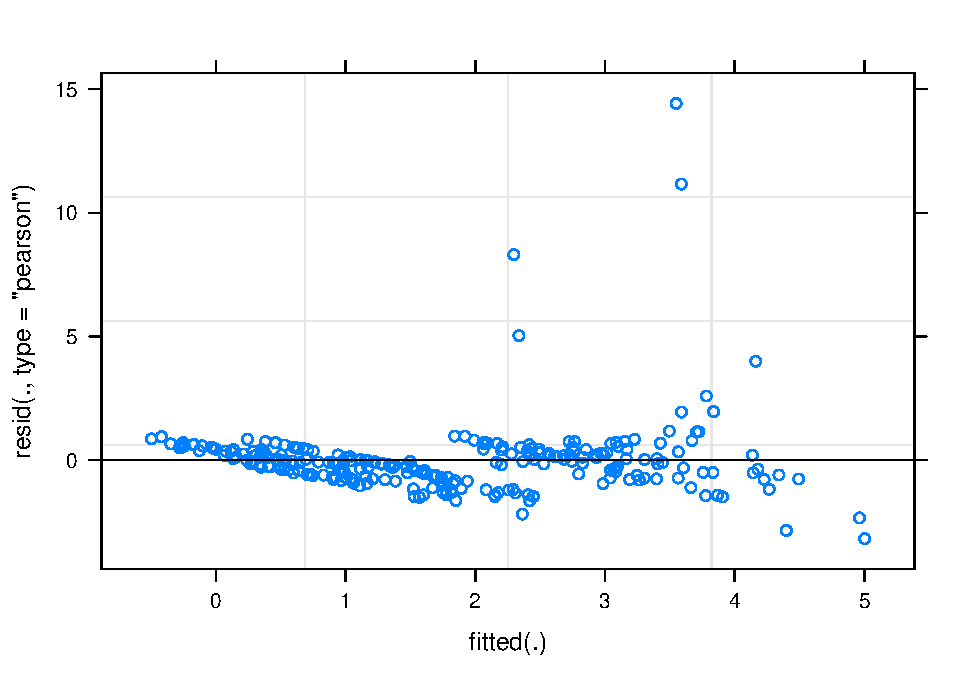
\includegraphics{project_draft_files/figure-latex/unnamed-chunk-6-1.pdf}

\begin{Shaded}
\begin{Highlighting}[]
\FunctionTok{par}\NormalTok{(}\AttributeTok{mfrow =} \FunctionTok{c}\NormalTok{(}\DecValTok{1}\NormalTok{,}\DecValTok{1}\NormalTok{))}
\end{Highlighting}
\end{Shaded}

\newpage

\textless\textless\textless\textless\textless\textless\textless{} HEAD
\#\# Question 3: Which landscape-level characteristics and plant
functional traits influence density of individual lemur species?

\begin{Shaded}
\begin{Highlighting}[]
\CommentTok{\#Exploring drivers of density for individual species though the use of linear models}
\CommentTok{\#I will explore the drivers of density for the two species with the greatest densities and the two species with the lowest densities}

\NormalTok{checking\_lemur\_densities }\OtherTok{\textless{}{-}}
\NormalTok{  trait\_data2 }\SpecialCharTok{\%\textgreater{}\%} 
  \FunctionTok{group\_by}\NormalTok{(Species) }\SpecialCharTok{\%\textgreater{}\%} 
  \FunctionTok{summarize}\NormalTok{(}\FunctionTok{mean}\NormalTok{(Predicted))}

\CommentTok{\#Avahi\_laniger and Lepilemur\_microdon are the species with the lowest predicted densities. Eulemur\_rubriventer and Propithecus\_edwardsi are the species with the highest predicted densities. }
\CommentTok{\#I will create linear models for each of these four species to analyze species specific drivers of density}

\NormalTok{AL\_subset }\OtherTok{\textless{}{-}} \FunctionTok{filter}\NormalTok{(trait\_data2, Species }\SpecialCharTok{==} \StringTok{"Avahi\_laniger"}\NormalTok{)}

\NormalTok{AL\_lm\_1 }\OtherTok{\textless{}{-}} \FunctionTok{lm}\NormalTok{(}\AttributeTok{data =}\NormalTok{ AL\_subset, Predicted }\SpecialCharTok{\textasciitilde{}}\NormalTok{ logSeedLength }\SpecialCharTok{+}\NormalTok{ logNitrogen }\SpecialCharTok{+}\NormalTok{ lat }\SpecialCharTok{+}\NormalTok{ logSeedWidth }\SpecialCharTok{+}\NormalTok{ logTannins }\SpecialCharTok{+}\NormalTok{ roughness }\SpecialCharTok{+}\NormalTok{ long }\SpecialCharTok{+}\NormalTok{ logSugar }\SpecialCharTok{+}\NormalTok{ logSLA }\SpecialCharTok{+}\NormalTok{ slope }\SpecialCharTok{+}\NormalTok{ Site }\SpecialCharTok{+}\NormalTok{ logFruitLength }\SpecialCharTok{+}\NormalTok{ logFat }\SpecialCharTok{+}\NormalTok{ aspect }\SpecialCharTok{+}\NormalTok{ logFruitWidth }\SpecialCharTok{+}\NormalTok{ logProtein)}
\FunctionTok{summary}\NormalTok{(AL\_lm\_1)}
\end{Highlighting}
\end{Shaded}

\begin{verbatim}
## 
## Call:
## lm(formula = Predicted ~ logSeedLength + logNitrogen + lat + 
##     logSeedWidth + logTannins + roughness + long + logSugar + 
##     logSLA + slope + Site + logFruitLength + logFat + aspect + 
##     logFruitWidth + logProtein, data = AL_subset)
## 
## Residuals:
##        Min         1Q     Median         3Q        Max 
## -0.0183628 -0.0078726 -0.0004125  0.0075975  0.0227697 
## 
## Coefficients:
##                  Estimate Std. Error t value Pr(>|t|)  
## (Intercept)    -5.266e+01  2.869e+01  -1.836   0.1161  
## logSeedLength   3.733e-01  2.846e-01   1.312   0.2375  
## logNitrogen    -1.254e-02  2.884e-01  -0.043   0.9667  
## lat            -9.978e-01  6.246e-01  -1.597   0.1613  
## logSeedWidth   -4.049e-01  2.956e-01  -1.370   0.2199  
## logTannins     -6.037e-03  8.544e-01  -0.007   0.9946  
## roughness       4.225e-05  1.734e-04   0.244   0.8157  
## long            6.657e-01  6.591e-01   1.010   0.3515  
## logSugar       -1.034e-03  1.692e-01  -0.006   0.9953  
## logSLA          2.716e-01  2.210e-01   1.229   0.2650  
## slope          -1.946e-03  6.547e-03  -0.297   0.7763  
## SiteMaharira   -4.377e-01  2.183e-01  -2.005   0.0918 .
## SiteMiaranony  -2.544e-01  1.001e-01  -2.542   0.0440 *
## SiteValohoaka  -2.773e-01  1.839e-01  -1.508   0.1822  
## SiteVohiparara -2.588e-01  1.371e-01  -1.888   0.1079  
## logFruitLength -3.823e-01  2.540e-01  -1.505   0.1830  
## logFat         -1.116e-01  1.237e-01  -0.902   0.4016  
## aspect         -9.069e-07  2.848e-04  -0.003   0.9976  
## logFruitWidth   4.008e-01  1.874e-01   2.139   0.0763 .
## logProtein      4.985e-02  7.744e-02   0.644   0.5436  
## ---
## Signif. codes:  0 '***' 0.001 '**' 0.01 '*' 0.05 '.' 0.1 ' ' 1
## 
## Residual standard error: 0.02236 on 6 degrees of freedom
## Multiple R-squared:  0.9173, Adjusted R-squared:  0.6556 
## F-statistic: 3.504 on 19 and 6 DF,  p-value: 0.06328
\end{verbatim}

\begin{Shaded}
\begin{Highlighting}[]
\NormalTok{AL\_lm\_2 }\OtherTok{\textless{}{-}} \FunctionTok{update}\NormalTok{(AL\_lm\_1,}\SpecialCharTok{\textasciitilde{}}\NormalTok{.}\SpecialCharTok{{-}}\NormalTok{logSugar)}
\FunctionTok{summary}\NormalTok{(AL\_lm\_2)}
\end{Highlighting}
\end{Shaded}

\begin{verbatim}
## 
## Call:
## lm(formula = Predicted ~ logSeedLength + logNitrogen + lat + 
##     logSeedWidth + logTannins + roughness + long + logSLA + slope + 
##     Site + logFruitLength + logFat + aspect + logFruitWidth + 
##     logProtein, data = AL_subset)
## 
## Residuals:
##        Min         1Q     Median         3Q        Max 
## -0.0183629 -0.0078610 -0.0004582  0.0075967  0.0227761 
## 
## Coefficients:
##                  Estimate Std. Error t value Pr(>|t|)  
## (Intercept)    -5.268e+01  2.647e+01  -1.990   0.0869 .
## logSeedLength   3.735e-01  2.608e-01   1.432   0.1951  
## logNitrogen    -1.205e-02  2.568e-01  -0.047   0.9639  
## lat            -9.967e-01  5.526e-01  -1.804   0.1143  
## logSeedWidth   -4.049e-01  2.737e-01  -1.479   0.1826  
## logTannins     -7.318e-03  7.669e-01  -0.010   0.9927  
## roughness       4.202e-05  1.568e-04   0.268   0.7964  
## long            6.664e-01  5.985e-01   1.113   0.3023  
## logSLA          2.710e-01  1.793e-01   1.512   0.1744  
## slope          -1.931e-03  5.602e-03  -0.345   0.7404  
## SiteMaharira   -4.371e-01  1.822e-01  -2.399   0.0475 *
## SiteMiaranony  -2.545e-01  9.230e-02  -2.757   0.0282 *
## SiteValohoaka  -2.771e-01  1.669e-01  -1.660   0.1409  
## SiteVohiparara -2.586e-01  1.207e-01  -2.143   0.0694 .
## logFruitLength -3.823e-01  2.351e-01  -1.626   0.1480  
## logFat         -1.120e-01  9.755e-02  -1.149   0.2885  
## aspect         -1.133e-06  2.615e-04  -0.004   0.9967  
## logFruitWidth   4.009e-01  1.731e-01   2.316   0.0537 .
## logProtein      4.980e-02  7.130e-02   0.699   0.5074  
## ---
## Signif. codes:  0 '***' 0.001 '**' 0.01 '*' 0.05 '.' 0.1 ' ' 1
## 
## Residual standard error: 0.0207 on 7 degrees of freedom
## Multiple R-squared:  0.9173, Adjusted R-squared:  0.7048 
## F-statistic: 4.316 on 18 and 7 DF,  p-value: 0.02804
\end{verbatim}

\begin{Shaded}
\begin{Highlighting}[]
\NormalTok{AL\_lm\_3 }\OtherTok{\textless{}{-}} \FunctionTok{update}\NormalTok{(AL\_lm\_2,}\SpecialCharTok{\textasciitilde{}}\NormalTok{.}\SpecialCharTok{{-}}\NormalTok{logTannins)}
\FunctionTok{summary}\NormalTok{(AL\_lm\_3)}
\end{Highlighting}
\end{Shaded}

\begin{verbatim}
## 
## Call:
## lm(formula = Predicted ~ logSeedLength + logNitrogen + lat + 
##     logSeedWidth + roughness + long + logSLA + slope + Site + 
##     logFruitLength + logFat + aspect + logFruitWidth + logProtein, 
##     data = AL_subset)
## 
## Residuals:
##        Min         1Q     Median         3Q        Max 
## -0.0184039 -0.0078313 -0.0004705  0.0075981  0.0228028 
## 
## Coefficients:
##                  Estimate Std. Error t value Pr(>|t|)  
## (Intercept)    -5.274e+01  2.400e+01  -2.197   0.0592 .
## logSeedLength   3.738e-01  2.423e-01   1.543   0.1614  
## logNitrogen    -1.076e-02  2.041e-01  -0.053   0.9592  
## lat            -9.959e-01  5.104e-01  -1.951   0.0869 .
## logSeedWidth   -4.066e-01  1.951e-01  -2.084   0.0707 .
## roughness       4.147e-05  1.364e-04   0.304   0.7688  
## long            6.682e-01  5.316e-01   1.257   0.2442  
## logSLA          2.702e-01  1.490e-01   1.814   0.1073  
## slope          -1.918e-03  5.088e-03  -0.377   0.7159  
## SiteMaharira   -4.365e-01  1.602e-01  -2.724   0.0261 *
## SiteMiaranony  -2.541e-01  7.869e-02  -3.229   0.0121 *
## SiteValohoaka  -2.763e-01  1.366e-01  -2.023   0.0777 .
## SiteVohiparara -2.584e-01  1.117e-01  -2.314   0.0494 *
## logFruitLength -3.833e-01  1.971e-01  -1.944   0.0877 .
## logFat         -1.118e-01  8.871e-02  -1.261   0.2430  
## aspect          4.339e-07  1.903e-04   0.002   0.9982  
## logFruitWidth   4.012e-01  1.595e-01   2.514   0.0361 *
## logProtein      4.935e-02  5.010e-02   0.985   0.3534  
## ---
## Signif. codes:  0 '***' 0.001 '**' 0.01 '*' 0.05 '.' 0.1 ' ' 1
## 
## Residual standard error: 0.01936 on 8 degrees of freedom
## Multiple R-squared:  0.9173, Adjusted R-squared:  0.7417 
## F-statistic: 5.222 on 17 and 8 DF,  p-value: 0.01142
\end{verbatim}

\begin{Shaded}
\begin{Highlighting}[]
\NormalTok{AL\_lm\_4 }\OtherTok{\textless{}{-}} \FunctionTok{update}\NormalTok{(AL\_lm\_3,}\SpecialCharTok{\textasciitilde{}}\NormalTok{.}\SpecialCharTok{{-}}\NormalTok{aspect)}
\FunctionTok{summary}\NormalTok{(AL\_lm\_4)}
\end{Highlighting}
\end{Shaded}

\begin{verbatim}
## 
## Call:
## lm(formula = Predicted ~ logSeedLength + logNitrogen + lat + 
##     logSeedWidth + roughness + long + logSLA + slope + Site + 
##     logFruitLength + logFat + logFruitWidth + logProtein, data = AL_subset)
## 
## Residuals:
##        Min         1Q     Median         3Q        Max 
## -0.0184061 -0.0078314 -0.0004696  0.0075889  0.0228034 
## 
## Coefficients:
##                  Estimate Std. Error t value Pr(>|t|)   
## (Intercept)    -5.274e+01  2.263e+01  -2.331  0.04469 * 
## logSeedLength   3.735e-01  1.892e-01   1.974  0.07979 . 
## logNitrogen    -1.078e-02  1.922e-01  -0.056  0.95651   
## lat            -9.958e-01  4.792e-01  -2.078  0.06748 . 
## logSeedWidth   -4.064e-01  1.629e-01  -2.495  0.03415 * 
## roughness       4.158e-05  1.197e-04   0.347  0.73623   
## long            6.683e-01  5.012e-01   1.333  0.21516   
## logSLA          2.702e-01  1.402e-01   1.927  0.08603 . 
## slope          -1.922e-03  4.524e-03  -0.425  0.68094   
## SiteMaharira   -4.366e-01  1.507e-01  -2.897  0.01767 * 
## SiteMiaranony  -2.541e-01  7.419e-02  -3.425  0.00757 **
## SiteValohoaka  -2.764e-01  1.277e-01  -2.164  0.05872 . 
## SiteVohiparara -2.584e-01  1.051e-01  -2.458  0.03625 * 
## logFruitLength -3.831e-01  1.555e-01  -2.463  0.03598 * 
## logFat         -1.118e-01  7.941e-02  -1.407  0.19288   
## logFruitWidth   4.012e-01  1.470e-01   2.729  0.02326 * 
## logProtein      4.941e-02  3.960e-02   1.248  0.24353   
## ---
## Signif. codes:  0 '***' 0.001 '**' 0.01 '*' 0.05 '.' 0.1 ' ' 1
## 
## Residual standard error: 0.01826 on 9 degrees of freedom
## Multiple R-squared:  0.9173, Adjusted R-squared:  0.7704 
## F-statistic: 6.242 on 16 and 9 DF,  p-value: 0.004282
\end{verbatim}

\begin{Shaded}
\begin{Highlighting}[]
\NormalTok{AL\_lm\_5 }\OtherTok{\textless{}{-}} \FunctionTok{update}\NormalTok{(AL\_lm\_4,}\SpecialCharTok{\textasciitilde{}}\NormalTok{.}\SpecialCharTok{{-}}\NormalTok{logNitrogen)}
\FunctionTok{summary}\NormalTok{(AL\_lm\_5)}
\end{Highlighting}
\end{Shaded}

\begin{verbatim}
## 
## Call:
## lm(formula = Predicted ~ logSeedLength + lat + logSeedWidth + 
##     roughness + long + logSLA + slope + Site + logFruitLength + 
##     logFat + logFruitWidth + logProtein, data = AL_subset)
## 
## Residuals:
##        Min         1Q     Median         3Q        Max 
## -0.0183122 -0.0075201 -0.0005731  0.0073756  0.0225534 
## 
## Coefficients:
##                  Estimate Std. Error t value Pr(>|t|)   
## (Intercept)    -5.242e+01  2.078e+01  -2.522   0.0303 * 
## logSeedLength   3.747e-01  1.785e-01   2.099   0.0622 . 
## lat            -9.977e-01  4.534e-01  -2.200   0.0524 . 
## logSeedWidth   -4.070e-01  1.541e-01  -2.641   0.0247 * 
## roughness       4.141e-05  1.135e-04   0.365   0.7228   
## long            6.606e-01  4.576e-01   1.444   0.1794   
## logSLA          2.691e-01  1.317e-01   2.042   0.0684 . 
## slope          -1.948e-03  4.270e-03  -0.456   0.6580   
## SiteMaharira   -4.376e-01  1.420e-01  -3.082   0.0116 * 
## SiteMiaranony  -2.537e-01  7.012e-02  -3.619   0.0047 **
## SiteValohoaka  -2.772e-01  1.204e-01  -2.301   0.0441 * 
## SiteVohiparara -2.588e-01  9.955e-02  -2.599   0.0265 * 
## logFruitLength -3.819e-01  1.463e-01  -2.610   0.0260 * 
## logFat         -1.129e-01  7.288e-02  -1.549   0.1524   
## logFruitWidth   3.979e-01  1.275e-01   3.121   0.0108 * 
## logProtein      5.031e-02  3.437e-02   1.464   0.1739   
## ---
## Signif. codes:  0 '***' 0.001 '**' 0.01 '*' 0.05 '.' 0.1 ' ' 1
## 
## Residual standard error: 0.01732 on 10 degrees of freedom
## Multiple R-squared:  0.9173, Adjusted R-squared:  0.7933 
## F-statistic: 7.395 on 15 and 10 DF,  p-value: 0.001486
\end{verbatim}

\begin{Shaded}
\begin{Highlighting}[]
\NormalTok{AL\_lm\_6 }\OtherTok{\textless{}{-}} \FunctionTok{update}\NormalTok{(AL\_lm\_5,}\SpecialCharTok{\textasciitilde{}}\NormalTok{.}\SpecialCharTok{{-}}\NormalTok{roughness)}
\FunctionTok{summary}\NormalTok{(AL\_lm\_6)}
\end{Highlighting}
\end{Shaded}

\begin{verbatim}
## 
## Call:
## lm(formula = Predicted ~ logSeedLength + lat + logSeedWidth + 
##     long + logSLA + slope + Site + logFruitLength + logFat + 
##     logFruitWidth + logProtein, data = AL_subset)
## 
## Residuals:
##        Min         1Q     Median         3Q        Max 
## -0.0186348 -0.0075396 -0.0007129  0.0065590  0.0221233 
## 
## Coefficients:
##                  Estimate Std. Error t value Pr(>|t|)   
## (Intercept)    -5.267e+01  1.994e+01  -2.642  0.02292 * 
## logSeedLength   3.807e-01  1.706e-01   2.232  0.04733 * 
## lat            -1.027e+00  4.281e-01  -2.400  0.03525 * 
## logSeedWidth   -4.113e-01  1.475e-01  -2.788  0.01764 * 
## long            6.535e-01  4.388e-01   1.489  0.16449   
## logSLA          2.720e-01  1.262e-01   2.155  0.05413 . 
## slope          -5.606e-04  1.863e-03  -0.301  0.76910   
## SiteMaharira   -4.407e-01  1.360e-01  -3.241  0.00786 **
## SiteMiaranony  -2.509e-01  6.689e-02  -3.751  0.00320 **
## SiteValohoaka  -2.824e-01  1.148e-01  -2.460  0.03168 * 
## SiteVohiparara -2.637e-01  9.463e-02  -2.787  0.01768 * 
## logFruitLength -3.814e-01  1.404e-01  -2.716  0.02007 * 
## logFat         -1.098e-01  6.946e-02  -1.580  0.14238   
## logFruitWidth   3.814e-01  1.144e-01   3.333  0.00668 **
## logProtein      4.586e-02  3.084e-02   1.487  0.16505   
## ---
## Signif. codes:  0 '***' 0.001 '**' 0.01 '*' 0.05 '.' 0.1 ' ' 1
## 
## Residual standard error: 0.01663 on 11 degrees of freedom
## Multiple R-squared:  0.9162, Adjusted R-squared:  0.8096 
## F-statistic: 8.591 on 14 and 11 DF,  p-value: 0.0005089
\end{verbatim}

\begin{Shaded}
\begin{Highlighting}[]
\NormalTok{AL\_lm\_7 }\OtherTok{\textless{}{-}} \FunctionTok{update}\NormalTok{(AL\_lm\_6,}\SpecialCharTok{\textasciitilde{}}\NormalTok{.}\SpecialCharTok{{-}}\NormalTok{slope)}
\FunctionTok{summary}\NormalTok{(AL\_lm\_7)}
\end{Highlighting}
\end{Shaded}

\begin{verbatim}
## 
## Call:
## lm(formula = Predicted ~ logSeedLength + lat + logSeedWidth + 
##     long + logSLA + Site + logFruitLength + logFat + logFruitWidth + 
##     logProtein, data = AL_subset)
## 
## Residuals:
##       Min        1Q    Median        3Q       Max 
## -0.018766 -0.007359 -0.001678  0.005595  0.023094 
## 
## Coefficients:
##                 Estimate Std. Error t value Pr(>|t|)   
## (Intercept)    -53.59434   18.93478  -2.830  0.01516 * 
## logSeedLength    0.37747    0.16363   2.307  0.03970 * 
## lat             -1.00638    0.40608  -2.478  0.02905 * 
## logSeedWidth    -0.40820    0.14146  -2.886  0.01369 * 
## long             0.68351    0.41076   1.664  0.12198   
## logSLA           0.25729    0.11180   2.301  0.04010 * 
## SiteMaharira    -0.43526    0.12957  -3.359  0.00568 **
## SiteMiaranony   -0.25252    0.06411  -3.939  0.00197 **
## SiteValohoaka   -0.27893    0.10980  -2.540  0.02592 * 
## SiteVohiparara  -0.25684    0.08826  -2.910  0.01308 * 
## logFruitLength  -0.38817    0.13323  -2.914  0.01300 * 
## logFat          -0.11118    0.06663  -1.669  0.12102   
## logFruitWidth    0.38066    0.10999   3.461  0.00471 **
## logProtein       0.04671    0.02952   1.582  0.13954   
## ---
## Signif. codes:  0 '***' 0.001 '**' 0.01 '*' 0.05 '.' 0.1 ' ' 1
## 
## Residual standard error: 0.01598 on 12 degrees of freedom
## Multiple R-squared:  0.9155, Adjusted R-squared:  0.824 
## F-statistic:    10 on 13 and 12 DF,  p-value: 0.000159
\end{verbatim}

\begin{Shaded}
\begin{Highlighting}[]
\NormalTok{AL\_lm\_8 }\OtherTok{\textless{}{-}} \FunctionTok{update}\NormalTok{(AL\_lm\_7,}\SpecialCharTok{\textasciitilde{}}\NormalTok{.}\SpecialCharTok{{-}}\NormalTok{logProtein)}
\FunctionTok{summary}\NormalTok{(AL\_lm\_8)}
\end{Highlighting}
\end{Shaded}

\begin{verbatim}
## 
## Call:
## lm(formula = Predicted ~ logSeedLength + lat + logSeedWidth + 
##     long + logSLA + Site + logFruitLength + logFat + logFruitWidth, 
##     data = AL_subset)
## 
## Residuals:
##       Min        1Q    Median        3Q       Max 
## -0.021608 -0.008082 -0.001649  0.008836  0.027191 
## 
## Coefficients:
##                 Estimate Std. Error t value Pr(>|t|)   
## (Intercept)    -48.96124   19.75957  -2.478  0.02772 * 
## logSeedLength    0.49371    0.15444   3.197  0.00701 **
## lat             -1.11014    0.42330  -2.623  0.02108 * 
## logSeedWidth    -0.45543    0.14605  -3.118  0.00816 **
## long             0.54806    0.42435   1.292  0.21901   
## logSLA           0.20917    0.11363   1.841  0.08860 . 
## SiteMaharira    -0.44741    0.13662  -3.275  0.00603 **
## SiteMiaranony   -0.24035    0.06723  -3.575  0.00339 **
## SiteValohoaka   -0.29196    0.11565  -2.524  0.02539 * 
## SiteVohiparara  -0.26653    0.09300  -2.866  0.01325 * 
## logFruitLength  -0.47527    0.12816  -3.709  0.00263 **
## logFat          -0.07757    0.06670  -1.163  0.26577   
## logFruitWidth    0.34529    0.11376   3.035  0.00957 **
## ---
## Signif. codes:  0 '***' 0.001 '**' 0.01 '*' 0.05 '.' 0.1 ' ' 1
## 
## Residual standard error: 0.01688 on 13 degrees of freedom
## Multiple R-squared:  0.8979, Adjusted R-squared:  0.8036 
## F-statistic: 9.526 on 12 and 13 DF,  p-value: 0.0001391
\end{verbatim}

\begin{Shaded}
\begin{Highlighting}[]
\NormalTok{AL\_lm\_9 }\OtherTok{\textless{}{-}} \FunctionTok{update}\NormalTok{(AL\_lm\_8,}\SpecialCharTok{\textasciitilde{}}\NormalTok{.}\SpecialCharTok{{-}}\NormalTok{logFat)}
\FunctionTok{summary}\NormalTok{(AL\_lm\_9)}
\end{Highlighting}
\end{Shaded}

\begin{verbatim}
## 
## Call:
## lm(formula = Predicted ~ logSeedLength + lat + logSeedWidth + 
##     long + logSLA + Site + logFruitLength + logFruitWidth, data = AL_subset)
## 
## Residuals:
##        Min         1Q     Median         3Q        Max 
## -0.0278399 -0.0059317 -0.0006755  0.0065675  0.0242129 
## 
## Coefficients:
##                 Estimate Std. Error t value Pr(>|t|)   
## (Intercept)    -48.65563   20.00492  -2.432  0.02902 * 
## logSeedLength    0.48554    0.15621   3.108  0.00771 **
## lat             -1.15117    0.42710  -2.695  0.01742 * 
## logSeedWidth    -0.44093    0.14734  -2.993  0.00969 **
## long             0.51948    0.42893   1.211  0.24590   
## logSLA           0.20199    0.11489   1.758  0.10055   
## SiteMaharira    -0.45539    0.13815  -3.296  0.00530 **
## SiteMiaranony   -0.24668    0.06784  -3.636  0.00270 **
## SiteValohoaka   -0.30835    0.11622  -2.653  0.01891 * 
## SiteVohiparara  -0.27027    0.09411  -2.872  0.01231 * 
## logFruitLength  -0.40120    0.11260  -3.563  0.00312 **
## logFruitWidth    0.29131    0.10516   2.770  0.01503 * 
## ---
## Signif. codes:  0 '***' 0.001 '**' 0.01 '*' 0.05 '.' 0.1 ' ' 1
## 
## Residual standard error: 0.01709 on 14 degrees of freedom
## Multiple R-squared:  0.8873, Adjusted R-squared:  0.7987 
## F-statistic: 10.02 on 11 and 14 DF,  p-value: 7.534e-05
\end{verbatim}

\begin{Shaded}
\begin{Highlighting}[]
\NormalTok{AL\_lm\_10 }\OtherTok{\textless{}{-}} \FunctionTok{update}\NormalTok{(AL\_lm\_9,}\SpecialCharTok{\textasciitilde{}}\NormalTok{.}\SpecialCharTok{{-}}\NormalTok{long)}
\FunctionTok{summary}\NormalTok{(AL\_lm\_10)}
\end{Highlighting}
\end{Shaded}

\begin{verbatim}
## 
## Call:
## lm(formula = Predicted ~ logSeedLength + lat + logSeedWidth + 
##     logSLA + Site + logFruitLength + logFruitWidth, data = AL_subset)
## 
## Residuals:
##       Min        1Q    Median        3Q       Max 
## -0.024985 -0.008192 -0.001441  0.009811  0.025280 
## 
## Coefficients:
##                 Estimate Std. Error t value Pr(>|t|)   
## (Intercept)    -26.78267    8.73649  -3.066  0.00785 **
## logSeedLength    0.54270    0.15121   3.589  0.00269 **
## lat             -1.27377    0.42134  -3.023  0.00856 **
## logSeedWidth    -0.47180    0.14736  -3.202  0.00594 **
## logSLA           0.26009    0.10600   2.454  0.02685 * 
## SiteMaharira    -0.49563    0.13617  -3.640  0.00242 **
## SiteMiaranony   -0.20344    0.05858  -3.473  0.00341 **
## SiteValohoaka   -0.32752    0.11692  -2.801  0.01343 * 
## SiteVohiparara  -0.30482    0.09107  -3.347  0.00441 **
## logFruitLength  -0.41023    0.11409  -3.596  0.00265 **
## logFruitWidth    0.29228    0.10678   2.737  0.01527 * 
## ---
## Signif. codes:  0 '***' 0.001 '**' 0.01 '*' 0.05 '.' 0.1 ' ' 1
## 
## Residual standard error: 0.01736 on 15 degrees of freedom
## Multiple R-squared:  0.8755, Adjusted R-squared:  0.7924 
## F-statistic: 10.54 on 10 and 15 DF,  p-value: 4.189e-05
\end{verbatim}

\begin{Shaded}
\begin{Highlighting}[]
\FunctionTok{AIC}\NormalTok{(AL\_lm\_2, AL\_lm\_3, AL\_lm\_4, AL\_lm\_5, AL\_lm\_6, AL\_lm\_7, AL\_lm\_8, AL\_lm\_9, AL\_lm\_10)}
\end{Highlighting}
\end{Shaded}

\begin{verbatim}
##          df       AIC
## AL_lm_2  20 -121.9668
## AL_lm_3  19 -123.9664
## AL_lm_4  18 -125.9664
## AL_lm_5  17 -127.9573
## AL_lm_6  16 -129.6135
## AL_lm_7  15 -131.4004
## AL_lm_8  14 -128.4729
## AL_lm_9  13 -127.8998
## AL_lm_10 12 -127.3093
\end{verbatim}

\begin{Shaded}
\begin{Highlighting}[]
\CommentTok{\#AL\_lm\_7 has the lowest AIC, and explains 82\% of the variation of Avahi laniger densities }
\CommentTok{\#AL\_lm\_10 has only significant variables, and explains 79\% of the variation of Avahi laniger densities}
\CommentTok{\#I selected model AL\_lm\_10}
\CommentTok{\#logSeedLength, lat, logSeedWidth, logSLA, SiteMaharira, SiteMiaranony, SiteValohoaka, SiteVohiparara, logFruitLength, and logFruitWidth are significant variables}

\NormalTok{ER\_subset }\OtherTok{\textless{}{-}} \FunctionTok{filter}\NormalTok{(trait\_data2, Species }\SpecialCharTok{==} \StringTok{"Eulemur\_rubriventer"}\NormalTok{)}

\NormalTok{ER\_lm\_1 }\OtherTok{\textless{}{-}} \FunctionTok{lm}\NormalTok{(}\AttributeTok{data =}\NormalTok{ ER\_subset, Predicted }\SpecialCharTok{\textasciitilde{}}\NormalTok{ logSeedLength }\SpecialCharTok{+}\NormalTok{ logNitrogen }\SpecialCharTok{+}\NormalTok{ lat }\SpecialCharTok{+}\NormalTok{ logSeedWidth }\SpecialCharTok{+}\NormalTok{ logTannins }\SpecialCharTok{+}\NormalTok{ roughness }\SpecialCharTok{+}\NormalTok{ long }\SpecialCharTok{+}\NormalTok{ logSugar }\SpecialCharTok{+}\NormalTok{ logSLA }\SpecialCharTok{+}\NormalTok{ slope }\SpecialCharTok{+}\NormalTok{ Site }\SpecialCharTok{+}\NormalTok{ logFruitLength }\SpecialCharTok{+}\NormalTok{ logFat }\SpecialCharTok{+}\NormalTok{ aspect }\SpecialCharTok{+}\NormalTok{ logFruitWidth }\SpecialCharTok{+}\NormalTok{ logProtein)}
\FunctionTok{summary}\NormalTok{(ER\_lm\_1)}
\end{Highlighting}
\end{Shaded}

\begin{verbatim}
## 
## Call:
## lm(formula = Predicted ~ logSeedLength + logNitrogen + lat + 
##     logSeedWidth + logTannins + roughness + long + logSugar + 
##     logSLA + slope + Site + logFruitLength + logFat + aspect + 
##     logFruitWidth + logProtein, data = ER_subset)
## 
## Residuals:
##      Min       1Q   Median       3Q      Max 
## -1.11606 -0.44945 -0.09879  0.35030  1.53307 
## 
## Coefficients:
##                  Estimate Std. Error t value Pr(>|t|)   
## (Intercept)    -2.452e+03  1.276e+03  -1.922  0.08083 . 
## logSeedLength   7.417e+00  8.321e+00   0.891  0.39185   
## logNitrogen    -3.880e+00  1.197e+01  -0.324  0.75191   
## lat            -6.441e+01  2.641e+01  -2.439  0.03288 * 
## logSeedWidth   -1.668e+01  9.670e+00  -1.725  0.11250   
## logTannins      3.481e+01  2.128e+01   1.636  0.13019   
## roughness       3.789e-03  7.127e-03   0.532  0.60557   
## long            2.350e+01  2.710e+01   0.867  0.40426   
## logSugar       -5.728e+00  5.113e+00  -1.120  0.28645   
## logSLA          6.004e+00  9.273e+00   0.647  0.53059   
## slope          -3.554e-01  2.810e-01  -1.265  0.23215   
## SiteMaharira   -2.492e+01  9.215e+00  -2.704  0.02052 * 
## SiteMiaranony  -1.006e+01  4.175e+00  -2.410  0.03459 * 
## SiteValohoaka  -1.539e+01  7.614e+00  -2.021  0.06827 . 
## SiteVohiparara -1.609e+01  5.927e+00  -2.715  0.02011 * 
## logFruitLength -2.781e+01  9.286e+00  -2.995  0.01219 * 
## logFat         -5.819e-01  4.860e+00  -0.120  0.90686   
## aspect          4.942e-04  5.139e-03   0.096  0.92511   
## logFruitWidth   2.947e+01  8.582e+00   3.433  0.00559 **
## logProtein      8.693e-01  2.203e+00   0.395  0.70074   
## ---
## Signif. codes:  0 '***' 0.001 '**' 0.01 '*' 0.05 '.' 0.1 ' ' 1
## 
## Residual standard error: 1.075 on 11 degrees of freedom
## Multiple R-squared:  0.7795, Adjusted R-squared:  0.3986 
## F-statistic: 2.047 on 19 and 11 DF,  p-value: 0.1123
\end{verbatim}

\begin{Shaded}
\begin{Highlighting}[]
\NormalTok{ER\_lm\_2 }\OtherTok{\textless{}{-}} \FunctionTok{update}\NormalTok{(ER\_lm\_1,}\SpecialCharTok{\textasciitilde{}}\NormalTok{.}\SpecialCharTok{{-}}\NormalTok{aspect)}
\FunctionTok{summary}\NormalTok{(ER\_lm\_2)}
\end{Highlighting}
\end{Shaded}

\begin{verbatim}
## 
## Call:
## lm(formula = Predicted ~ logSeedLength + logNitrogen + lat + 
##     logSeedWidth + logTannins + roughness + long + logSugar + 
##     logSLA + slope + Site + logFruitLength + logFat + logFruitWidth + 
##     logProtein, data = ER_subset)
## 
## Residuals:
##     Min      1Q  Median      3Q     Max 
## -1.1168 -0.4553 -0.1004  0.3480  1.5300 
## 
## Coefficients:
##                  Estimate Std. Error t value Pr(>|t|)   
## (Intercept)    -2.420e+03  1.180e+03  -2.052  0.06269 . 
## logSeedLength   7.208e+00  7.694e+00   0.937  0.36731   
## logNitrogen    -3.657e+00  1.125e+01  -0.325  0.75070   
## lat            -6.433e+01  2.528e+01  -2.544  0.02573 * 
## logSeedWidth   -1.648e+01  9.054e+00  -1.821  0.09369 . 
## logTannins      3.483e+01  2.038e+01   1.709  0.11315   
## roughness       3.846e-03  6.802e-03   0.565  0.58220   
## long            2.285e+01  2.512e+01   0.910  0.38098   
## logSugar       -5.690e+00  4.883e+00  -1.165  0.26652   
## logSLA          5.912e+00  8.835e+00   0.669  0.51603   
## slope          -3.585e-01  2.673e-01  -1.341  0.20477   
## SiteMaharira   -2.490e+01  8.826e+00  -2.822  0.01541 * 
## SiteMiaranony  -9.961e+00  3.868e+00  -2.575  0.02431 * 
## SiteValohoaka  -1.541e+01  7.291e+00  -2.113  0.05620 . 
## SiteVohiparara -1.604e+01  5.654e+00  -2.837  0.01498 * 
## logFruitLength -2.752e+01  8.404e+00  -3.274  0.00665 **
## logFat         -4.411e-01  4.439e+00  -0.099  0.92248   
## logFruitWidth   2.938e+01  8.171e+00   3.595  0.00368 **
## logProtein      8.973e-01  2.092e+00   0.429  0.67560   
## ---
## Signif. codes:  0 '***' 0.001 '**' 0.01 '*' 0.05 '.' 0.1 ' ' 1
## 
## Residual standard error: 1.03 on 12 degrees of freedom
## Multiple R-squared:  0.7793, Adjusted R-squared:  0.4483 
## F-statistic: 2.354 on 18 and 12 DF,  p-value: 0.06708
\end{verbatim}

\begin{Shaded}
\begin{Highlighting}[]
\NormalTok{ER\_lm\_3 }\OtherTok{\textless{}{-}} \FunctionTok{update}\NormalTok{(ER\_lm\_2,}\SpecialCharTok{\textasciitilde{}}\NormalTok{.}\SpecialCharTok{{-}}\NormalTok{logFat)}
\FunctionTok{summary}\NormalTok{(ER\_lm\_3)}
\end{Highlighting}
\end{Shaded}

\begin{verbatim}
## 
## Call:
## lm(formula = Predicted ~ logSeedLength + logNitrogen + lat + 
##     logSeedWidth + logTannins + roughness + long + logSugar + 
##     logSLA + slope + Site + logFruitLength + logFruitWidth + 
##     logProtein, data = ER_subset)
## 
## Residuals:
##      Min       1Q   Median       3Q      Max 
## -1.12655 -0.44307 -0.08421  0.35848  1.55283 
## 
## Coefficients:
##                  Estimate Std. Error t value Pr(>|t|)   
## (Intercept)    -2.455e+03  1.082e+03  -2.270  0.04088 * 
## logSeedLength   7.001e+00  7.118e+00   0.983  0.34332   
## logNitrogen    -3.987e+00  1.033e+01  -0.386  0.70572   
## lat            -6.442e+01  2.428e+01  -2.653  0.01991 * 
## logSeedWidth   -1.636e+01  8.621e+00  -1.898  0.08017 . 
## logTannins      3.546e+01  1.864e+01   1.903  0.07945 . 
## roughness       3.947e-03  6.464e-03   0.611  0.55195   
## long            2.354e+01  2.320e+01   1.014  0.32891   
## logSugar       -5.854e+00  4.418e+00  -1.325  0.20800   
## logSLA          5.994e+00  8.455e+00   0.709  0.49094   
## slope          -3.624e-01  2.542e-01  -1.426  0.17746   
## SiteMaharira   -2.495e+01  8.474e+00  -2.944  0.01141 * 
## SiteMiaranony  -1.005e+01  3.611e+00  -2.784  0.01551 * 
## SiteValohoaka  -1.546e+01  6.991e+00  -2.211  0.04555 * 
## SiteVohiparara -1.605e+01  5.434e+00  -2.953  0.01120 * 
## logFruitLength -2.726e+01  7.679e+00  -3.549  0.00356 **
## logFruitWidth   2.929e+01  7.815e+00   3.748  0.00243 **
## logProtein      8.636e-01  1.984e+00   0.435  0.67054   
## ---
## Signif. codes:  0 '***' 0.001 '**' 0.01 '*' 0.05 '.' 0.1 ' ' 1
## 
## Residual standard error: 0.9898 on 13 degrees of freedom
## Multiple R-squared:  0.7791, Adjusted R-squared:  0.4903 
## F-statistic: 2.698 on 17 and 13 DF,  p-value: 0.03779
\end{verbatim}

\begin{Shaded}
\begin{Highlighting}[]
\NormalTok{ER\_lm\_4 }\OtherTok{\textless{}{-}} \FunctionTok{update}\NormalTok{(ER\_lm\_3,}\SpecialCharTok{\textasciitilde{}}\NormalTok{.}\SpecialCharTok{{-}}\NormalTok{logNitrogen)}
\FunctionTok{summary}\NormalTok{(ER\_lm\_4)}
\end{Highlighting}
\end{Shaded}

\begin{verbatim}
## 
## Call:
## lm(formula = Predicted ~ logSeedLength + lat + logSeedWidth + 
##     logTannins + roughness + long + logSugar + logSLA + slope + 
##     Site + logFruitLength + logFruitWidth + logProtein, data = ER_subset)
## 
## Residuals:
##      Min       1Q   Median       3Q      Max 
## -1.12981 -0.45212 -0.05761  0.40728  1.49928 
## 
## Coefficients:
##                  Estimate Std. Error t value Pr(>|t|)   
## (Intercept)    -2.415e+03  1.043e+03  -2.314  0.03635 * 
## logSeedLength   7.771e+00  6.622e+00   1.174  0.26012   
## lat            -6.397e+01  2.351e+01  -2.721  0.01655 * 
## logSeedWidth   -1.753e+01  7.825e+00  -2.240  0.04183 * 
## logTannins      3.765e+01  1.720e+01   2.189  0.04605 * 
## roughness       3.572e-03  6.193e-03   0.577  0.57329   
## long            2.286e+01  2.242e+01   1.020  0.32525   
## logSugar       -5.329e+00  4.074e+00  -1.308  0.21192   
## logSLA          5.133e+00  7.905e+00   0.649  0.52660   
## slope          -3.578e-01  2.460e-01  -1.454  0.16797   
## SiteMaharira   -2.477e+01  8.200e+00  -3.020  0.00918 **
## SiteMiaranony  -9.962e+00  3.492e+00  -2.853  0.01279 * 
## SiteValohoaka  -1.539e+01  6.772e+00  -2.272  0.03940 * 
## SiteVohiparara -1.597e+01  5.263e+00  -3.035  0.00891 **
## logFruitLength -2.695e+01  7.403e+00  -3.641  0.00267 **
## logFruitWidth   2.837e+01  7.213e+00   3.934  0.00150 **
## logProtein      9.784e-01  1.901e+00   0.515  0.61488   
## ---
## Signif. codes:  0 '***' 0.001 '**' 0.01 '*' 0.05 '.' 0.1 ' ' 1
## 
## Residual standard error: 0.9592 on 14 degrees of freedom
## Multiple R-squared:  0.7766, Adjusted R-squared:  0.5213 
## F-statistic: 3.042 on 16 and 14 DF,  p-value: 0.02123
\end{verbatim}

\begin{Shaded}
\begin{Highlighting}[]
\NormalTok{ER\_lm\_5 }\OtherTok{\textless{}{-}} \FunctionTok{update}\NormalTok{(ER\_lm\_4,}\SpecialCharTok{\textasciitilde{}}\NormalTok{.}\SpecialCharTok{{-}}\NormalTok{logProtein)}
\FunctionTok{summary}\NormalTok{(ER\_lm\_5)}
\end{Highlighting}
\end{Shaded}

\begin{verbatim}
## 
## Call:
## lm(formula = Predicted ~ logSeedLength + lat + logSeedWidth + 
##     logTannins + roughness + long + logSugar + logSLA + slope + 
##     Site + logFruitLength + logFruitWidth, data = ER_subset)
## 
## Residuals:
##      Min       1Q   Median       3Q      Max 
## -1.10261 -0.46309 -0.00053  0.32655  1.51726 
## 
## Coefficients:
##                  Estimate Std. Error t value Pr(>|t|)    
## (Intercept)    -2.515e+03  9.999e+02  -2.515 0.023802 *  
## logSeedLength   8.582e+00  6.272e+00   1.368 0.191354    
## lat            -6.195e+01  2.260e+01  -2.741 0.015163 *  
## logSeedWidth   -1.874e+01  7.277e+00  -2.575 0.021108 *  
## logTannins      4.203e+01  1.458e+01   2.883 0.011379 *  
## roughness       2.408e-03  5.622e-03   0.428 0.674543    
## long            2.603e+01  2.103e+01   1.238 0.234724    
## logSugar       -4.363e+00  3.526e+00  -1.237 0.234956    
## logSLA          3.518e+00  7.075e+00   0.497 0.626198    
## slope          -3.113e-01  2.232e-01  -1.395 0.183404    
## SiteMaharira   -2.344e+01  7.592e+00  -3.088 0.007505 ** 
## SiteMiaranony  -9.578e+00  3.327e+00  -2.879 0.011475 *  
## SiteValohoaka  -1.443e+01  6.350e+00  -2.272 0.038226 *  
## SiteVohiparara -1.542e+01  5.023e+00  -3.069 0.007794 ** 
## logFruitLength -2.867e+01  6.448e+00  -4.446 0.000472 ***
## logFruitWidth   2.886e+01  6.973e+00   4.139 0.000875 ***
## ---
## Signif. codes:  0 '***' 0.001 '**' 0.01 '*' 0.05 '.' 0.1 ' ' 1
## 
## Residual standard error: 0.9354 on 15 degrees of freedom
## Multiple R-squared:  0.7724, Adjusted R-squared:  0.5448 
## F-statistic: 3.393 on 15 and 15 DF,  p-value: 0.01187
\end{verbatim}

\begin{Shaded}
\begin{Highlighting}[]
\NormalTok{ER\_lm\_6 }\OtherTok{\textless{}{-}} \FunctionTok{update}\NormalTok{(ER\_lm\_5,}\SpecialCharTok{\textasciitilde{}}\NormalTok{.}\SpecialCharTok{{-}}\NormalTok{roughness)}
\FunctionTok{summary}\NormalTok{(ER\_lm\_6)}
\end{Highlighting}
\end{Shaded}

\begin{verbatim}
## 
## Call:
## lm(formula = Predicted ~ logSeedLength + lat + logSeedWidth + 
##     logTannins + long + logSugar + logSLA + slope + Site + logFruitLength + 
##     logFruitWidth, data = ER_subset)
## 
## Residuals:
##      Min       1Q   Median       3Q      Max 
## -1.18733 -0.42150  0.01556  0.28845  1.53172 
## 
## Coefficients:
##                  Estimate Std. Error t value Pr(>|t|)    
## (Intercept)    -2600.3392   954.2845  -2.725 0.014987 *  
## logSeedLength      7.8139     5.8545   1.335 0.200667    
## lat              -62.4887    21.9861  -2.842 0.011770 *  
## logSeedWidth     -18.2158     6.9875  -2.607 0.019071 *  
## logTannins        41.7733    14.1894   2.944 0.009529 ** 
## long              27.5933    20.1727   1.368 0.190264    
## logSugar          -4.0510     3.3607  -1.205 0.245565    
## logSLA             3.6538     6.8851   0.531 0.602926    
## slope             -0.2269     0.1020  -2.224 0.040885 *  
## SiteMaharira     -23.2783     7.3865  -3.151 0.006176 ** 
## SiteMiaranony     -9.5938     3.2409  -2.960 0.009213 ** 
## SiteValohoaka    -14.5673     6.1777  -2.358 0.031432 *  
## SiteVohiparara   -15.4960     4.8902  -3.169 0.005956 ** 
## logFruitLength   -27.8168     5.9762  -4.655 0.000264 ***
## logFruitWidth     28.0591     6.5438   4.288 0.000565 ***
## ---
## Signif. codes:  0 '***' 0.001 '**' 0.01 '*' 0.05 '.' 0.1 ' ' 1
## 
## Residual standard error: 0.9112 on 16 degrees of freedom
## Multiple R-squared:  0.7696, Adjusted R-squared:  0.568 
## F-statistic: 3.817 on 14 and 16 DF,  p-value: 0.006109
\end{verbatim}

\begin{Shaded}
\begin{Highlighting}[]
\NormalTok{ER\_lm\_7 }\OtherTok{\textless{}{-}} \FunctionTok{update}\NormalTok{(ER\_lm\_6,}\SpecialCharTok{\textasciitilde{}}\NormalTok{.}\SpecialCharTok{{-}}\NormalTok{logSLA)}
\FunctionTok{summary}\NormalTok{(ER\_lm\_7)}
\end{Highlighting}
\end{Shaded}

\begin{verbatim}
## 
## Call:
## lm(formula = Predicted ~ logSeedLength + lat + logSeedWidth + 
##     logTannins + long + logSugar + slope + Site + logFruitLength + 
##     logFruitWidth, data = ER_subset)
## 
## Residuals:
##      Min       1Q   Median       3Q      Max 
## -1.13432 -0.42182 -0.09341  0.34694  1.64062 
## 
## Coefficients:
##                  Estimate Std. Error t value Pr(>|t|)    
## (Intercept)    -2.846e+03  8.168e+02  -3.484 0.002841 ** 
## logSeedLength   6.595e+00  5.270e+00   1.251 0.227743    
## lat            -6.092e+01  2.132e+01  -2.857 0.010907 *  
## logSeedWidth   -1.778e+01  6.791e+00  -2.618 0.017984 *  
## logTannins      4.099e+01  1.381e+01   2.968 0.008624 ** 
## long            3.364e+01  1.629e+01   2.066 0.054425 .  
## logSugar       -3.353e+00  3.027e+00  -1.108 0.283342    
## slope          -2.001e-01  8.674e-02  -2.307 0.033917 *  
## SiteMaharira   -2.261e+01  7.121e+00  -3.174 0.005546 ** 
## SiteMiaranony  -9.905e+00  3.119e+00  -3.175 0.005537 ** 
## SiteValohoaka  -1.420e+01  6.009e+00  -2.364 0.030245 *  
## SiteVohiparara -1.482e+01  4.619e+00  -3.208 0.005161 ** 
## logFruitLength -2.805e+01  5.833e+00  -4.809 0.000164 ***
## logFruitWidth   2.841e+01  6.370e+00   4.460 0.000344 ***
## ---
## Signif. codes:  0 '***' 0.001 '**' 0.01 '*' 0.05 '.' 0.1 ' ' 1
## 
## Residual standard error: 0.8918 on 17 degrees of freedom
## Multiple R-squared:  0.7655, Adjusted R-squared:  0.5862 
## F-statistic:  4.27 on 13 and 17 DF,  p-value: 0.003106
\end{verbatim}

\begin{Shaded}
\begin{Highlighting}[]
\NormalTok{ER\_lm\_8 }\OtherTok{\textless{}{-}} \FunctionTok{update}\NormalTok{(ER\_lm\_7,}\SpecialCharTok{\textasciitilde{}}\NormalTok{.}\SpecialCharTok{{-}}\NormalTok{logSugar)}
\FunctionTok{summary}\NormalTok{(ER\_lm\_8)}
\end{Highlighting}
\end{Shaded}

\begin{verbatim}
## 
## Call:
## lm(formula = Predicted ~ logSeedLength + lat + logSeedWidth + 
##     logTannins + long + slope + Site + logFruitLength + logFruitWidth, 
##     data = ER_subset)
## 
## Residuals:
##     Min      1Q  Median      3Q     Max 
## -1.2881 -0.4963 -0.1182  0.3891  1.8263 
## 
## Coefficients:
##                  Estimate Std. Error t value Pr(>|t|)    
## (Intercept)    -2.528e+03  7.697e+02  -3.285 0.004118 ** 
## logSeedLength   6.542e+00  5.303e+00   1.234 0.233205    
## lat            -5.366e+01  2.042e+01  -2.628 0.017055 *  
## logSeedWidth   -1.851e+01  6.802e+00  -2.722 0.013988 *  
## logTannins      4.091e+01  1.390e+01   2.943 0.008689 ** 
## long            2.985e+01  1.602e+01   1.863 0.078866 .  
## slope          -1.933e-01  8.707e-02  -2.220 0.039490 *  
## SiteMaharira   -1.951e+01  6.591e+00  -2.960 0.008386 ** 
## SiteMiaranony  -8.809e+00  2.977e+00  -2.959 0.008405 ** 
## SiteValohoaka  -1.208e+01  5.731e+00  -2.108 0.049284 *  
## SiteVohiparara -1.356e+01  4.505e+00  -3.009 0.007535 ** 
## logFruitLength -2.568e+01  5.461e+00  -4.703 0.000177 ***
## logFruitWidth   2.911e+01  6.379e+00   4.564 0.000240 ***
## ---
## Signif. codes:  0 '***' 0.001 '**' 0.01 '*' 0.05 '.' 0.1 ' ' 1
## 
## Residual standard error: 0.8974 on 18 degrees of freedom
## Multiple R-squared:  0.7486, Adjusted R-squared:  0.581 
## F-statistic: 4.467 on 12 and 18 DF,  p-value: 0.002246
\end{verbatim}

\begin{Shaded}
\begin{Highlighting}[]
\NormalTok{ER\_lm\_9 }\OtherTok{\textless{}{-}} \FunctionTok{update}\NormalTok{(ER\_lm\_8,}\SpecialCharTok{\textasciitilde{}}\NormalTok{.}\SpecialCharTok{{-}}\NormalTok{logSeedLength)}
\FunctionTok{summary}\NormalTok{(ER\_lm\_9)}
\end{Highlighting}
\end{Shaded}

\begin{verbatim}
## 
## Call:
## lm(formula = Predicted ~ lat + logSeedWidth + logTannins + long + 
##     slope + Site + logFruitLength + logFruitWidth, data = ER_subset)
## 
## Residuals:
##     Min      1Q  Median      3Q     Max 
## -1.1818 -0.4380 -0.1329  0.4505  1.8942 
## 
## Coefficients:
##                  Estimate Std. Error t value Pr(>|t|)    
## (Intercept)    -2.597e+03  7.782e+02  -3.337 0.003463 ** 
## lat            -5.330e+01  2.069e+01  -2.575 0.018530 *  
## logSeedWidth   -1.284e+01  5.082e+00  -2.527 0.020530 *  
## logTannins      3.917e+01  1.401e+01   2.795 0.011557 *  
## long            3.146e+01  1.619e+01   1.944 0.066895 .  
## slope          -2.095e-01  8.725e-02  -2.401 0.026742 *  
## SiteMaharira   -1.865e+01  6.643e+00  -2.807 0.011250 *  
## SiteMiaranony  -8.371e+00  2.996e+00  -2.794 0.011578 *  
## SiteValohoaka  -1.190e+01  5.807e+00  -2.049 0.054512 .  
## SiteVohiparara -1.326e+01  4.560e+00  -2.907 0.009029 ** 
## logFruitLength -2.411e+01  5.383e+00  -4.480 0.000257 ***
## logFruitWidth   2.872e+01  6.458e+00   4.448 0.000276 ***
## ---
## Signif. codes:  0 '***' 0.001 '**' 0.01 '*' 0.05 '.' 0.1 ' ' 1
## 
## Residual standard error: 0.9096 on 19 degrees of freedom
## Multiple R-squared:  0.7274, Adjusted R-squared:  0.5695 
## F-statistic: 4.608 on 11 and 19 DF,  p-value: 0.0018
\end{verbatim}

\begin{Shaded}
\begin{Highlighting}[]
\NormalTok{ER\_lm\_10 }\OtherTok{\textless{}{-}} \FunctionTok{update}\NormalTok{(ER\_lm\_9,}\SpecialCharTok{\textasciitilde{}}\NormalTok{.}\SpecialCharTok{{-}}\NormalTok{long)}
\FunctionTok{summary}\NormalTok{(ER\_lm\_10)}
\end{Highlighting}
\end{Shaded}

\begin{verbatim}
## 
## Call:
## lm(formula = Predicted ~ lat + logSeedWidth + logTannins + slope + 
##     Site + logFruitLength + logFruitWidth, data = ER_subset)
## 
## Residuals:
##      Min       1Q   Median       3Q      Max 
## -1.39714 -0.46323 -0.02793  0.50480  1.67159 
## 
## Coefficients:
##                  Estimate Std. Error t value Pr(>|t|)    
## (Intercept)    -1322.5869   447.4299  -2.956 0.007812 ** 
## lat              -63.3686    21.3807  -2.964 0.007675 ** 
## logSeedWidth      -8.5481     4.8839  -1.750 0.095398 .  
## logTannins        27.3007    13.4626   2.028 0.056104 .  
## slope             -0.2114     0.0931  -2.271 0.034368 *  
## SiteMaharira     -21.7962     6.8758  -3.170 0.004815 ** 
## SiteMiaranony     -6.5317     3.0339  -2.153 0.043715 *  
## SiteValohoaka    -14.5118     6.0295  -2.407 0.025877 *  
## SiteVohiparara   -15.4614     4.7133  -3.280 0.003741 ** 
## logFruitLength   -23.0551     5.7153  -4.034 0.000650 ***
## logFruitWidth     27.3213     6.8487   3.989 0.000721 ***
## ---
## Signif. codes:  0 '***' 0.001 '**' 0.01 '*' 0.05 '.' 0.1 ' ' 1
## 
## Residual standard error: 0.9708 on 20 degrees of freedom
## Multiple R-squared:  0.6731, Adjusted R-squared:  0.5097 
## F-statistic: 4.119 on 10 and 20 DF,  p-value: 0.003431
\end{verbatim}

\begin{Shaded}
\begin{Highlighting}[]
\NormalTok{ER\_lm\_11 }\OtherTok{\textless{}{-}} \FunctionTok{update}\NormalTok{(ER\_lm\_10,}\SpecialCharTok{\textasciitilde{}}\NormalTok{.}\SpecialCharTok{{-}}\NormalTok{logSeedWidth)}
\FunctionTok{summary}\NormalTok{(ER\_lm\_11)}
\end{Highlighting}
\end{Shaded}

\begin{verbatim}
## 
## Call:
## lm(formula = Predicted ~ lat + logTannins + slope + Site + logFruitLength + 
##     logFruitWidth, data = ER_subset)
## 
## Residuals:
##      Min       1Q   Median       3Q      Max 
## -2.11036 -0.56636 -0.00057  0.53954  1.75513 
## 
## Coefficients:
##                  Estimate Std. Error t value Pr(>|t|)   
## (Intercept)    -1.432e+03  4.643e+02  -3.084  0.00562 **
## lat            -6.851e+01  2.219e+01  -3.087  0.00559 **
## logTannins      7.525e+00  7.672e+00   0.981  0.33779   
## slope          -1.989e-01  9.728e-02  -2.044  0.05368 . 
## SiteMaharira   -2.295e+01  7.173e+00  -3.199  0.00431 **
## SiteMiaranony  -7.960e+00  3.062e+00  -2.600  0.01673 * 
## SiteValohoaka  -1.699e+01  6.142e+00  -2.767  0.01155 * 
## SiteVohiparara -1.540e+01  4.939e+00  -3.117  0.00521 **
## logFruitLength -1.923e+01  5.535e+00  -3.475  0.00226 **
## logFruitWidth   1.862e+01  4.934e+00   3.773  0.00112 **
## ---
## Signif. codes:  0 '***' 0.001 '**' 0.01 '*' 0.05 '.' 0.1 ' ' 1
## 
## Residual standard error: 1.017 on 21 degrees of freedom
## Multiple R-squared:  0.6231, Adjusted R-squared:  0.4615 
## F-statistic: 3.857 on 9 and 21 DF,  p-value: 0.005161
\end{verbatim}

\begin{Shaded}
\begin{Highlighting}[]
\NormalTok{ER\_lm\_12 }\OtherTok{\textless{}{-}} \FunctionTok{update}\NormalTok{(ER\_lm\_11,}\SpecialCharTok{\textasciitilde{}}\NormalTok{.}\SpecialCharTok{{-}}\NormalTok{logTannins)}
\FunctionTok{summary}\NormalTok{(ER\_lm\_12)}
\end{Highlighting}
\end{Shaded}

\begin{verbatim}
## 
## Call:
## lm(formula = Predicted ~ lat + slope + Site + logFruitLength + 
##     logFruitWidth, data = ER_subset)
## 
## Residuals:
##      Min       1Q   Median       3Q      Max 
## -2.19232 -0.45601  0.06244  0.50266  1.68377 
## 
## Coefficients:
##                  Estimate Std. Error t value Pr(>|t|)    
## (Intercept)    -1.417e+03  4.636e+02  -3.056 0.005787 ** 
## lat            -6.772e+01  2.216e+01  -3.056 0.005791 ** 
## slope          -2.167e-01  9.548e-02  -2.270 0.033374 *  
## SiteMaharira   -2.250e+01  7.152e+00  -3.146 0.004688 ** 
## SiteMiaranony  -8.144e+00  3.054e+00  -2.667 0.014089 *  
## SiteValohoaka  -1.697e+01  6.136e+00  -2.765 0.011304 *  
## SiteVohiparara -1.536e+01  4.935e+00  -3.113 0.005070 ** 
## logFruitLength -1.855e+01  5.486e+00  -3.381 0.002693 ** 
## logFruitWidth   1.888e+01  4.923e+00   3.835 0.000902 ***
## ---
## Signif. codes:  0 '***' 0.001 '**' 0.01 '*' 0.05 '.' 0.1 ' ' 1
## 
## Residual standard error: 1.016 on 22 degrees of freedom
## Multiple R-squared:  0.6058, Adjusted R-squared:  0.4625 
## F-statistic: 4.226 on 8 and 22 DF,  p-value: 0.003409
\end{verbatim}

\begin{Shaded}
\begin{Highlighting}[]
\CommentTok{\#all variables are significant}

\FunctionTok{AIC}\NormalTok{(ER\_lm\_1, ER\_lm\_2, ER\_lm\_3, ER\_lm\_4, ER\_lm\_5, ER\_lm\_6, ER\_lm\_7, ER\_lm\_8, ER\_lm\_9, ER\_lm\_10, ER\_lm\_11, ER\_lm\_12)}
\end{Highlighting}
\end{Shaded}

\begin{verbatim}
##          df       AIC
## ER_lm_1  21 102.34611
## ER_lm_2  20 100.37216
## ER_lm_3  19  98.39766
## ER_lm_4  18  96.75100
## ER_lm_5  17  95.33182
## ER_lm_6  16  93.70858
## ER_lm_7  15  92.24948
## ER_lm_8  14  92.41058
## ER_lm_9  13  92.92663
## ER_lm_10 12  96.54857
## ER_lm_11 11  98.96660
## ER_lm_12 10  98.35546
\end{verbatim}

\begin{Shaded}
\begin{Highlighting}[]
\CommentTok{\#7, 8, and 9 have has the lowest AIC}
\FunctionTok{summary}\NormalTok{(ER\_lm\_7)}
\end{Highlighting}
\end{Shaded}

\begin{verbatim}
## 
## Call:
## lm(formula = Predicted ~ logSeedLength + lat + logSeedWidth + 
##     logTannins + long + logSugar + slope + Site + logFruitLength + 
##     logFruitWidth, data = ER_subset)
## 
## Residuals:
##      Min       1Q   Median       3Q      Max 
## -1.13432 -0.42182 -0.09341  0.34694  1.64062 
## 
## Coefficients:
##                  Estimate Std. Error t value Pr(>|t|)    
## (Intercept)    -2.846e+03  8.168e+02  -3.484 0.002841 ** 
## logSeedLength   6.595e+00  5.270e+00   1.251 0.227743    
## lat            -6.092e+01  2.132e+01  -2.857 0.010907 *  
## logSeedWidth   -1.778e+01  6.791e+00  -2.618 0.017984 *  
## logTannins      4.099e+01  1.381e+01   2.968 0.008624 ** 
## long            3.364e+01  1.629e+01   2.066 0.054425 .  
## logSugar       -3.353e+00  3.027e+00  -1.108 0.283342    
## slope          -2.001e-01  8.674e-02  -2.307 0.033917 *  
## SiteMaharira   -2.261e+01  7.121e+00  -3.174 0.005546 ** 
## SiteMiaranony  -9.905e+00  3.119e+00  -3.175 0.005537 ** 
## SiteValohoaka  -1.420e+01  6.009e+00  -2.364 0.030245 *  
## SiteVohiparara -1.482e+01  4.619e+00  -3.208 0.005161 ** 
## logFruitLength -2.805e+01  5.833e+00  -4.809 0.000164 ***
## logFruitWidth   2.841e+01  6.370e+00   4.460 0.000344 ***
## ---
## Signif. codes:  0 '***' 0.001 '**' 0.01 '*' 0.05 '.' 0.1 ' ' 1
## 
## Residual standard error: 0.8918 on 17 degrees of freedom
## Multiple R-squared:  0.7655, Adjusted R-squared:  0.5862 
## F-statistic:  4.27 on 13 and 17 DF,  p-value: 0.003106
\end{verbatim}

\begin{Shaded}
\begin{Highlighting}[]
\FunctionTok{summary}\NormalTok{(ER\_lm\_8)}
\end{Highlighting}
\end{Shaded}

\begin{verbatim}
## 
## Call:
## lm(formula = Predicted ~ logSeedLength + lat + logSeedWidth + 
##     logTannins + long + slope + Site + logFruitLength + logFruitWidth, 
##     data = ER_subset)
## 
## Residuals:
##     Min      1Q  Median      3Q     Max 
## -1.2881 -0.4963 -0.1182  0.3891  1.8263 
## 
## Coefficients:
##                  Estimate Std. Error t value Pr(>|t|)    
## (Intercept)    -2.528e+03  7.697e+02  -3.285 0.004118 ** 
## logSeedLength   6.542e+00  5.303e+00   1.234 0.233205    
## lat            -5.366e+01  2.042e+01  -2.628 0.017055 *  
## logSeedWidth   -1.851e+01  6.802e+00  -2.722 0.013988 *  
## logTannins      4.091e+01  1.390e+01   2.943 0.008689 ** 
## long            2.985e+01  1.602e+01   1.863 0.078866 .  
## slope          -1.933e-01  8.707e-02  -2.220 0.039490 *  
## SiteMaharira   -1.951e+01  6.591e+00  -2.960 0.008386 ** 
## SiteMiaranony  -8.809e+00  2.977e+00  -2.959 0.008405 ** 
## SiteValohoaka  -1.208e+01  5.731e+00  -2.108 0.049284 *  
## SiteVohiparara -1.356e+01  4.505e+00  -3.009 0.007535 ** 
## logFruitLength -2.568e+01  5.461e+00  -4.703 0.000177 ***
## logFruitWidth   2.911e+01  6.379e+00   4.564 0.000240 ***
## ---
## Signif. codes:  0 '***' 0.001 '**' 0.01 '*' 0.05 '.' 0.1 ' ' 1
## 
## Residual standard error: 0.8974 on 18 degrees of freedom
## Multiple R-squared:  0.7486, Adjusted R-squared:  0.581 
## F-statistic: 4.467 on 12 and 18 DF,  p-value: 0.002246
\end{verbatim}

\begin{Shaded}
\begin{Highlighting}[]
\FunctionTok{summary}\NormalTok{(ER\_lm\_9)}
\end{Highlighting}
\end{Shaded}

\begin{verbatim}
## 
## Call:
## lm(formula = Predicted ~ lat + logSeedWidth + logTannins + long + 
##     slope + Site + logFruitLength + logFruitWidth, data = ER_subset)
## 
## Residuals:
##     Min      1Q  Median      3Q     Max 
## -1.1818 -0.4380 -0.1329  0.4505  1.8942 
## 
## Coefficients:
##                  Estimate Std. Error t value Pr(>|t|)    
## (Intercept)    -2.597e+03  7.782e+02  -3.337 0.003463 ** 
## lat            -5.330e+01  2.069e+01  -2.575 0.018530 *  
## logSeedWidth   -1.284e+01  5.082e+00  -2.527 0.020530 *  
## logTannins      3.917e+01  1.401e+01   2.795 0.011557 *  
## long            3.146e+01  1.619e+01   1.944 0.066895 .  
## slope          -2.095e-01  8.725e-02  -2.401 0.026742 *  
## SiteMaharira   -1.865e+01  6.643e+00  -2.807 0.011250 *  
## SiteMiaranony  -8.371e+00  2.996e+00  -2.794 0.011578 *  
## SiteValohoaka  -1.190e+01  5.807e+00  -2.049 0.054512 .  
## SiteVohiparara -1.326e+01  4.560e+00  -2.907 0.009029 ** 
## logFruitLength -2.411e+01  5.383e+00  -4.480 0.000257 ***
## logFruitWidth   2.872e+01  6.458e+00   4.448 0.000276 ***
## ---
## Signif. codes:  0 '***' 0.001 '**' 0.01 '*' 0.05 '.' 0.1 ' ' 1
## 
## Residual standard error: 0.9096 on 19 degrees of freedom
## Multiple R-squared:  0.7274, Adjusted R-squared:  0.5695 
## F-statistic: 4.608 on 11 and 19 DF,  p-value: 0.0018
\end{verbatim}

\begin{Shaded}
\begin{Highlighting}[]
\FunctionTok{summary}\NormalTok{(ER\_lm\_10)}
\end{Highlighting}
\end{Shaded}

\begin{verbatim}
## 
## Call:
## lm(formula = Predicted ~ lat + logSeedWidth + logTannins + slope + 
##     Site + logFruitLength + logFruitWidth, data = ER_subset)
## 
## Residuals:
##      Min       1Q   Median       3Q      Max 
## -1.39714 -0.46323 -0.02793  0.50480  1.67159 
## 
## Coefficients:
##                  Estimate Std. Error t value Pr(>|t|)    
## (Intercept)    -1322.5869   447.4299  -2.956 0.007812 ** 
## lat              -63.3686    21.3807  -2.964 0.007675 ** 
## logSeedWidth      -8.5481     4.8839  -1.750 0.095398 .  
## logTannins        27.3007    13.4626   2.028 0.056104 .  
## slope             -0.2114     0.0931  -2.271 0.034368 *  
## SiteMaharira     -21.7962     6.8758  -3.170 0.004815 ** 
## SiteMiaranony     -6.5317     3.0339  -2.153 0.043715 *  
## SiteValohoaka    -14.5118     6.0295  -2.407 0.025877 *  
## SiteVohiparara   -15.4614     4.7133  -3.280 0.003741 ** 
## logFruitLength   -23.0551     5.7153  -4.034 0.000650 ***
## logFruitWidth     27.3213     6.8487   3.989 0.000721 ***
## ---
## Signif. codes:  0 '***' 0.001 '**' 0.01 '*' 0.05 '.' 0.1 ' ' 1
## 
## Residual standard error: 0.9708 on 20 degrees of freedom
## Multiple R-squared:  0.6731, Adjusted R-squared:  0.5097 
## F-statistic: 4.119 on 10 and 20 DF,  p-value: 0.003431
\end{verbatim}

\begin{Shaded}
\begin{Highlighting}[]
\CommentTok{\#I selected ER\_lm\_9 because it had the best combination of a low AIC value and all significant variables (it had the lowest AIC and all significant variables, except for two marginally significant ones)}
\CommentTok{\#lat, logseed width, logtannins, long (marginally), slope, SiteMaharira, SiteMiaranony, SiteValohoaka (marginally), SiteVohiparara, logFruitLength, logFruitWidth are significant}
\CommentTok{\#this model explains 79\% of the y variable!}

\CommentTok{\#Propithecus\_edwardsi has the second highest density}
\NormalTok{PE\_subset }\OtherTok{\textless{}{-}} \FunctionTok{filter}\NormalTok{(trait\_data2, Species }\SpecialCharTok{==} \StringTok{"Propithecus\_edwardsi"}\NormalTok{)}

\NormalTok{PE\_lm\_1}\OtherTok{\textless{}{-}} \FunctionTok{lm}\NormalTok{(}\AttributeTok{data =}\NormalTok{ PE\_subset, Predicted }\SpecialCharTok{\textasciitilde{}}\NormalTok{ logSeedLength }\SpecialCharTok{+}\NormalTok{ logNitrogen }\SpecialCharTok{+}\NormalTok{ lat }\SpecialCharTok{+}\NormalTok{ logSeedWidth }\SpecialCharTok{+}\NormalTok{ logTannins }\SpecialCharTok{+}\NormalTok{ roughness }\SpecialCharTok{+}\NormalTok{ long }\SpecialCharTok{+}\NormalTok{ logSugar }\SpecialCharTok{+}\NormalTok{ logSLA }\SpecialCharTok{+}\NormalTok{ slope }\SpecialCharTok{+}\NormalTok{ Site }\SpecialCharTok{+}\NormalTok{ logFruitLength }\SpecialCharTok{+}\NormalTok{ logFat }\SpecialCharTok{+}\NormalTok{ aspect }\SpecialCharTok{+}\NormalTok{ logFruitWidth }\SpecialCharTok{+}\NormalTok{ logProtein)}
\FunctionTok{summary}\NormalTok{(PE\_lm\_1)}
\end{Highlighting}
\end{Shaded}

\begin{verbatim}
## 
## Call:
## lm(formula = Predicted ~ logSeedLength + logNitrogen + lat + 
##     logSeedWidth + logTannins + roughness + long + logSugar + 
##     logSLA + slope + Site + logFruitLength + logFat + aspect + 
##     logFruitWidth + logProtein, data = PE_subset)
## 
## Residuals:
##       Min        1Q    Median        3Q       Max 
## -0.257675 -0.092568 -0.007372  0.135958  0.293599 
## 
## Coefficients:
##                  Estimate Std. Error t value Pr(>|t|)  
## (Intercept)    -5.792e+02  3.054e+02  -1.896   0.0845 .
## logSeedLength   2.066e+00  1.992e+00   1.037   0.3220  
## logNitrogen     7.657e-01  2.866e+00   0.267   0.7943  
## lat            -1.586e+01  6.323e+00  -2.508   0.0291 *
## logSeedWidth   -4.613e+00  2.315e+00  -1.992   0.0717 .
## logTannins      9.282e+00  5.095e+00   1.822   0.0958 .
## roughness       4.721e-04  1.706e-03   0.277   0.7872  
## long            5.220e+00  6.488e+00   0.805   0.4381  
## logSugar       -1.140e+00  1.224e+00  -0.931   0.3719  
## logSLA          2.029e+00  2.220e+00   0.914   0.3804  
## slope          -3.954e-02  6.728e-02  -0.588   0.5686  
## SiteMaharira   -6.367e+00  2.206e+00  -2.886   0.0148 *
## SiteMiaranony  -2.412e+00  9.996e-01  -2.413   0.0344 *
## SiteValohoaka  -3.783e+00  1.823e+00  -2.075   0.0622 .
## SiteVohiparara -3.980e+00  1.419e+00  -2.804   0.0171 *
## logFruitLength -3.932e+00  2.223e+00  -1.768   0.1047  
## logFat         -1.920e-01  1.164e+00  -0.165   0.8720  
## aspect          1.493e-04  1.231e-03   0.121   0.9056  
## logFruitWidth   4.601e+00  2.055e+00   2.239   0.0468 *
## logProtein      2.933e-01  5.276e-01   0.556   0.5894  
## ---
## Signif. codes:  0 '***' 0.001 '**' 0.01 '*' 0.05 '.' 0.1 ' ' 1
## 
## Residual standard error: 0.2574 on 11 degrees of freedom
## Multiple R-squared:  0.8635, Adjusted R-squared:  0.6277 
## F-statistic: 3.662 on 19 and 11 DF,  p-value: 0.01588
\end{verbatim}

\begin{Shaded}
\begin{Highlighting}[]
\NormalTok{PE\_lm\_2 }\OtherTok{\textless{}{-}} \FunctionTok{update}\NormalTok{(PE\_lm\_1,}\SpecialCharTok{\textasciitilde{}}\NormalTok{.}\SpecialCharTok{{-}}\NormalTok{aspect)}
\FunctionTok{summary}\NormalTok{(PE\_lm\_2)}
\end{Highlighting}
\end{Shaded}

\begin{verbatim}
## 
## Call:
## lm(formula = Predicted ~ logSeedLength + logNitrogen + lat + 
##     logSeedWidth + logTannins + roughness + long + logSugar + 
##     logSLA + slope + Site + logFruitLength + logFat + logFruitWidth + 
##     logProtein, data = PE_subset)
## 
## Residuals:
##      Min       1Q   Median       3Q      Max 
## -0.25789 -0.09303 -0.00336  0.13867  0.29269 
## 
## Coefficients:
##                  Estimate Std. Error t value Pr(>|t|)  
## (Intercept)    -5.696e+02  2.825e+02  -2.016   0.0668 .
## logSeedLength   2.003e+00  1.843e+00   1.087   0.2984  
## logNitrogen     8.332e-01  2.694e+00   0.309   0.7624  
## lat            -1.583e+01  6.055e+00  -2.615   0.0226 *
## logSeedWidth   -4.554e+00  2.168e+00  -2.100   0.0575 .
## logTannins      9.290e+00  4.881e+00   1.903   0.0813 .
## roughness       4.895e-04  1.629e-03   0.300   0.7690  
## long            5.023e+00  6.016e+00   0.835   0.4201  
## logSugar       -1.128e+00  1.169e+00  -0.965   0.3537  
## logSLA          2.001e+00  2.116e+00   0.946   0.3629  
## slope          -4.049e-02  6.403e-02  -0.632   0.5390  
## SiteMaharira   -6.364e+00  2.114e+00  -3.011   0.0109 *
## SiteMiaranony  -2.381e+00  9.264e-01  -2.571   0.0245 *
## SiteValohoaka  -3.789e+00  1.746e+00  -2.170   0.0508 .
## SiteVohiparara -3.964e+00  1.354e+00  -2.928   0.0127 *
## logFruitLength -3.843e+00  2.013e+00  -1.910   0.0804 .
## logFat         -1.494e-01  1.063e+00  -0.141   0.8905  
## logFruitWidth   4.574e+00  1.957e+00   2.337   0.0376 *
## logProtein      3.017e-01  5.010e-01   0.602   0.5583  
## ---
## Signif. codes:  0 '***' 0.001 '**' 0.01 '*' 0.05 '.' 0.1 ' ' 1
## 
## Residual standard error: 0.2466 on 12 degrees of freedom
## Multiple R-squared:  0.8633, Adjusted R-squared:  0.6583 
## F-statistic: 4.211 on 18 and 12 DF,  p-value: 0.007305
\end{verbatim}

\begin{Shaded}
\begin{Highlighting}[]
\NormalTok{PE\_lm\_3 }\OtherTok{\textless{}{-}} \FunctionTok{update}\NormalTok{(PE\_lm\_2,}\SpecialCharTok{\textasciitilde{}}\NormalTok{.}\SpecialCharTok{{-}}\NormalTok{logFat)}
\FunctionTok{summary}\NormalTok{(PE\_lm\_3)}
\end{Highlighting}
\end{Shaded}

\begin{verbatim}
## 
## Call:
## lm(formula = Predicted ~ logSeedLength + logNitrogen + lat + 
##     logSeedWidth + logTannins + roughness + long + logSugar + 
##     logSLA + slope + Site + logFruitLength + logFruitWidth + 
##     logProtein, data = PE_subset)
## 
## Residuals:
##      Min       1Q   Median       3Q      Max 
## -0.26120 -0.08857 -0.01069  0.13935  0.30040 
## 
## Coefficients:
##                  Estimate Std. Error t value Pr(>|t|)   
## (Intercept)    -5.815e+02  2.592e+02  -2.243  0.04293 * 
## logSeedLength   1.933e+00  1.705e+00   1.133  0.27754   
## logNitrogen     7.214e-01  2.475e+00   0.292  0.77527   
## lat            -1.586e+01  5.818e+00  -2.726  0.01730 * 
## logSeedWidth   -4.512e+00  2.066e+00  -2.185  0.04783 * 
## logTannins      9.502e+00  4.465e+00   2.128  0.05303 . 
## roughness       5.238e-04  1.549e-03   0.338  0.74063   
## long            5.256e+00  5.560e+00   0.945  0.36168   
## logSugar       -1.184e+00  1.059e+00  -1.118  0.28374   
## logSLA          2.029e+00  2.026e+00   1.001  0.33487   
## slope          -4.181e-02  6.089e-02  -0.687  0.50437   
## SiteMaharira   -6.378e+00  2.030e+00  -3.141  0.00780 **
## SiteMiaranony  -2.412e+00  8.652e-01  -2.788  0.01537 * 
## SiteValohoaka  -3.806e+00  1.675e+00  -2.272  0.04070 * 
## SiteVohiparara -3.966e+00  1.302e+00  -3.047  0.00936 **
## logFruitLength -3.756e+00  1.840e+00  -2.041  0.06207 . 
## logFruitWidth   4.547e+00  1.872e+00   2.428  0.03043 * 
## logProtein      2.903e-01  4.754e-01   0.611  0.55196   
## ---
## Signif. codes:  0 '***' 0.001 '**' 0.01 '*' 0.05 '.' 0.1 ' ' 1
## 
## Residual standard error: 0.2371 on 13 degrees of freedom
## Multiple R-squared:  0.8631, Adjusted R-squared:  0.6841 
## F-statistic: 4.821 on 17 and 13 DF,  p-value: 0.003163
\end{verbatim}

\begin{Shaded}
\begin{Highlighting}[]
\NormalTok{PE\_lm\_4 }\OtherTok{\textless{}{-}} \FunctionTok{update}\NormalTok{(PE\_lm\_3,}\SpecialCharTok{\textasciitilde{}}\NormalTok{.}\SpecialCharTok{{-}}\NormalTok{logNitrogen)}
\FunctionTok{summary}\NormalTok{(PE\_lm\_4)}
\end{Highlighting}
\end{Shaded}

\begin{verbatim}
## 
## Call:
## lm(formula = Predicted ~ logSeedLength + lat + logSeedWidth + 
##     logTannins + roughness + long + logSugar + logSLA + slope + 
##     Site + logFruitLength + logFruitWidth + logProtein, data = PE_subset)
## 
## Residuals:
##      Min       1Q   Median       3Q      Max 
## -0.26061 -0.10071 -0.01784  0.13681  0.31009 
## 
## Coefficients:
##                  Estimate Std. Error t value Pr(>|t|)   
## (Intercept)    -5.888e+02  2.494e+02  -2.361  0.03327 * 
## logSeedLength   1.793e+00  1.583e+00   1.133  0.27616   
## lat            -1.594e+01  5.619e+00  -2.838  0.01317 * 
## logSeedWidth   -4.301e+00  1.870e+00  -2.300  0.03735 * 
## logTannins      9.105e+00  4.111e+00   2.215  0.04387 * 
## roughness       5.917e-04  1.480e-03   0.400  0.69537   
## long            5.379e+00  5.360e+00   1.004  0.33261   
## logSugar       -1.278e+00  9.737e-01  -1.313  0.21030   
## logSLA          2.185e+00  1.889e+00   1.156  0.26691   
## slope          -4.265e-02  5.880e-02  -0.725  0.48018   
## SiteMaharira   -6.411e+00  1.960e+00  -3.271  0.00557 **
## SiteMiaranony  -2.429e+00  8.347e-01  -2.910  0.01142 * 
## SiteValohoaka  -3.819e+00  1.619e+00  -2.359  0.03337 * 
## SiteVohiparara -3.980e+00  1.258e+00  -3.164  0.00690 **
## logFruitLength -3.811e+00  1.769e+00  -2.154  0.04919 * 
## logFruitWidth   4.713e+00  1.724e+00   2.734  0.01614 * 
## logProtein      2.695e-01  4.544e-01   0.593  0.56253   
## ---
## Signif. codes:  0 '***' 0.001 '**' 0.01 '*' 0.05 '.' 0.1 ' ' 1
## 
## Residual standard error: 0.2293 on 14 degrees of freedom
## Multiple R-squared:  0.8622, Adjusted R-squared:  0.7047 
## F-statistic: 5.475 on 16 and 14 DF,  p-value: 0.001326
\end{verbatim}

\begin{Shaded}
\begin{Highlighting}[]
\NormalTok{PE\_lm\_5 }\OtherTok{\textless{}{-}} \FunctionTok{update}\NormalTok{(PE\_lm\_4,}\SpecialCharTok{\textasciitilde{}}\NormalTok{.}\SpecialCharTok{{-}}\NormalTok{roughness)}
\FunctionTok{summary}\NormalTok{(PE\_lm\_5)}
\end{Highlighting}
\end{Shaded}

\begin{verbatim}
## 
## Call:
## lm(formula = Predicted ~ logSeedLength + lat + logSeedWidth + 
##     logTannins + long + logSugar + logSLA + slope + Site + logFruitLength + 
##     logFruitWidth + logProtein, data = PE_subset)
## 
## Residuals:
##      Min       1Q   Median       3Q      Max 
## -0.27681 -0.09093 -0.01362  0.13810  0.31439 
## 
## Coefficients:
##                  Estimate Std. Error t value Pr(>|t|)   
## (Intercept)    -613.82134  234.54381  -2.617  0.01943 * 
## logSeedLength     1.68479    1.51480   1.112  0.28355   
## lat             -15.92105    5.45871  -2.917  0.01063 * 
## logSeedWidth     -4.27186    1.81560  -2.353  0.03270 * 
## logTannins        9.34760    3.95071   2.366  0.03187 * 
## long              5.92625    5.03443   1.177  0.25748   
## logSugar         -1.14654    0.89004  -1.288  0.21720   
## logSLA            2.10392    1.82509   1.153  0.26704   
## slope            -0.02153    0.02505  -0.859  0.40368   
## SiteMaharira     -6.28613    1.87993  -3.344  0.00444 **
## SiteMiaranony    -2.40596    0.80911  -2.974  0.00947 **
## SiteValohoaka    -3.78344    1.57032  -2.409  0.02929 * 
## SiteVohiparara   -3.95896    1.22102  -3.242  0.00547 **
## logFruitLength   -3.74551    1.71189  -2.188  0.04492 * 
## logFruitWidth     4.57577    1.64113   2.788  0.01378 * 
## logProtein        0.20320    0.41102   0.494  0.62819   
## ---
## Signif. codes:  0 '***' 0.001 '**' 0.01 '*' 0.05 '.' 0.1 ' ' 1
## 
## Residual standard error: 0.2228 on 15 degrees of freedom
## Multiple R-squared:  0.8606, Adjusted R-squared:  0.7212 
## F-statistic: 6.175 on 15 and 15 DF,  p-value: 0.0005424
\end{verbatim}

\begin{Shaded}
\begin{Highlighting}[]
\NormalTok{PE\_lm\_6 }\OtherTok{\textless{}{-}} \FunctionTok{update}\NormalTok{(PE\_lm\_5,}\SpecialCharTok{\textasciitilde{}}\NormalTok{.}\SpecialCharTok{{-}}\NormalTok{logProtein)}
\FunctionTok{summary}\NormalTok{(PE\_lm\_6)}
\end{Highlighting}
\end{Shaded}

\begin{verbatim}
## 
## Call:
## lm(formula = Predicted ~ logSeedLength + lat + logSeedWidth + 
##     logTannins + long + logSugar + logSLA + slope + Site + logFruitLength + 
##     logFruitWidth, data = PE_subset)
## 
## Residuals:
##      Min       1Q   Median       3Q      Max 
## -0.26266 -0.10602 -0.04387  0.13888  0.31668 
## 
## Coefficients:
##                  Estimate Std. Error t value Pr(>|t|)   
## (Intercept)    -625.88954  227.69558  -2.749  0.01427 * 
## logSeedLength     1.93027    1.39691   1.382  0.18602   
## lat             -15.44855    5.24596  -2.945  0.00951 **
## logSeedWidth     -4.57619    1.66724  -2.745  0.01439 * 
## logTannins       10.28271    3.38563   3.037  0.00785 **
## long              6.42791    4.81328   1.335  0.20042   
## logSugar         -0.97721    0.80187  -1.219  0.24064   
## logSLA            1.75489    1.64280   1.068  0.30127   
## slope            -0.02036    0.02434  -0.836  0.41527   
## SiteMaharira     -6.02734    1.76244  -3.420  0.00351 **
## SiteMiaranony    -2.32467    0.77330  -3.006  0.00837 **
## SiteValohoaka    -3.57052    1.47403  -2.422  0.02766 * 
## SiteVohiparara   -3.83591    1.16682  -3.287  0.00464 **
## logFruitLength   -4.18674    1.42595  -2.936  0.00969 **
## logFruitWidth     4.75715    1.56137   3.047  0.00769 **
## ---
## Signif. codes:  0 '***' 0.001 '**' 0.01 '*' 0.05 '.' 0.1 ' ' 1
## 
## Residual standard error: 0.2174 on 16 degrees of freedom
## Multiple R-squared:  0.8584, Adjusted R-squared:  0.7344 
## F-statistic: 6.925 on 14 and 16 DF,  p-value: 0.0002179
\end{verbatim}

\begin{Shaded}
\begin{Highlighting}[]
\NormalTok{PE\_lm\_7 }\OtherTok{\textless{}{-}} \FunctionTok{update}\NormalTok{(PE\_lm\_6,}\SpecialCharTok{\textasciitilde{}}\NormalTok{.}\SpecialCharTok{{-}}\NormalTok{slope)}
\FunctionTok{summary}\NormalTok{(PE\_lm\_7)}
\end{Highlighting}
\end{Shaded}

\begin{verbatim}
## 
## Call:
## lm(formula = Predicted ~ logSeedLength + lat + logSeedWidth + 
##     logTannins + long + logSugar + logSLA + Site + logFruitLength + 
##     logFruitWidth, data = PE_subset)
## 
## Residuals:
##      Min       1Q   Median       3Q      Max 
## -0.26273 -0.11441 -0.01438  0.12357  0.36278 
## 
## Coefficients:
##                 Estimate Std. Error t value Pr(>|t|)   
## (Intercept)    -649.2846   223.9647  -2.899  0.00998 **
## logSeedLength     1.8431     1.3806   1.335  0.19951   
## lat             -14.2011     4.9848  -2.849  0.01110 * 
## logSeedWidth     -4.5692     1.6524  -2.765  0.01324 * 
## logTannins       10.2645     3.3555   3.059  0.00710 **
## long              7.5086     4.5954   1.634  0.12065   
## logSugar         -0.8093     0.7694  -1.052  0.30761   
## logSLA            1.0744     1.4145   0.760  0.45791   
## SiteMaharira     -5.6225     1.6796  -3.347  0.00382 **
## SiteMiaranony    -2.3254     0.7664  -3.034  0.00749 **
## SiteValohoaka    -3.3010     1.4256  -2.316  0.03334 * 
## SiteVohiparara   -3.4842     1.0788  -3.230  0.00492 **
## logFruitLength   -4.3215     1.4042  -3.077  0.00683 **
## logFruitWidth     4.7768     1.5473   3.087  0.00669 **
## ---
## Signif. codes:  0 '***' 0.001 '**' 0.01 '*' 0.05 '.' 0.1 ' ' 1
## 
## Residual standard error: 0.2155 on 17 degrees of freedom
## Multiple R-squared:  0.8522, Adjusted R-squared:  0.7391 
## F-statistic: 7.538 on 13 and 17 DF,  p-value: 0.0001024
\end{verbatim}

\begin{Shaded}
\begin{Highlighting}[]
\NormalTok{PE\_lm\_8 }\OtherTok{\textless{}{-}} \FunctionTok{update}\NormalTok{(PE\_lm\_7,}\SpecialCharTok{\textasciitilde{}}\NormalTok{.}\SpecialCharTok{{-}}\NormalTok{logSLA)}
\FunctionTok{summary}\NormalTok{(PE\_lm\_8)}
\end{Highlighting}
\end{Shaded}

\begin{verbatim}
## 
## Call:
## lm(formula = Predicted ~ logSeedLength + lat + logSeedWidth + 
##     logTannins + long + logSugar + Site + logFruitLength + logFruitWidth, 
##     data = PE_subset)
## 
## Residuals:
##      Min       1Q   Median       3Q      Max 
## -0.27923 -0.12564 -0.00001  0.12339  0.38155 
## 
## Coefficients:
##                 Estimate Std. Error t value Pr(>|t|)   
## (Intercept)    -732.9258   192.7193  -3.803  0.00130 **
## logSeedLength     1.4129     1.2443   1.136  0.27105   
## lat             -14.2290     4.9257  -2.889  0.00978 **
## logSeedWidth     -4.4037     1.6186  -2.721  0.01402 * 
## logTannins        9.9684     3.2934   3.027  0.00725 **
## long              9.3117     3.8883   2.395  0.02772 * 
## logSugar         -0.6236     0.7209  -0.865  0.39844   
## SiteMaharira     -5.5682     1.6583  -3.358  0.00350 **
## SiteMiaranony    -2.4462     0.7409  -3.302  0.00397 **
## SiteValohoaka    -3.2980     1.4087  -2.341  0.03094 * 
## SiteVohiparara   -3.4004     1.0604  -3.207  0.00489 **
## logFruitLength   -4.3436     1.3873  -3.131  0.00577 **
## logFruitWidth     4.9052     1.5199   3.227  0.00467 **
## ---
## Signif. codes:  0 '***' 0.001 '**' 0.01 '*' 0.05 '.' 0.1 ' ' 1
## 
## Residual standard error: 0.2129 on 18 degrees of freedom
## Multiple R-squared:  0.8471, Adjusted R-squared:  0.7452 
## F-statistic: 8.313 on 12 and 18 DF,  p-value: 4.364e-05
\end{verbatim}

\begin{Shaded}
\begin{Highlighting}[]
\NormalTok{PE\_lm\_9 }\OtherTok{\textless{}{-}} \FunctionTok{update}\NormalTok{(PE\_lm\_8,}\SpecialCharTok{\textasciitilde{}}\NormalTok{.}\SpecialCharTok{{-}}\NormalTok{logSugar)}
\FunctionTok{summary}\NormalTok{(PE\_lm\_9)}
\end{Highlighting}
\end{Shaded}

\begin{verbatim}
## 
## Call:
## lm(formula = Predicted ~ logSeedLength + lat + logSeedWidth + 
##     logTannins + long + Site + logFruitLength + logFruitWidth, 
##     data = PE_subset)
## 
## Residuals:
##      Min       1Q   Median       3Q      Max 
## -0.26752 -0.11826 -0.03062  0.13223  0.41413 
## 
## Coefficients:
##                 Estimate Std. Error t value Pr(>|t|)   
## (Intercept)    -675.4097   179.6813  -3.759  0.00133 **
## logSeedLength     1.3915     1.2358   1.126  0.27418   
## lat             -12.9520     4.6680  -2.775  0.01207 * 
## logSeedWidth     -4.5343     1.6009  -2.832  0.01064 * 
## logTannins        9.9425     3.2714   3.039  0.00675 **
## long              8.6058     3.7764   2.279  0.03441 * 
## SiteMaharira     -5.0124     1.5185  -3.301  0.00376 **
## SiteMiaranony    -2.2461     0.6992  -3.212  0.00459 **
## SiteValohoaka    -2.9182     1.3296  -2.195  0.04081 * 
## SiteVohiparara   -3.1832     1.0234  -3.110  0.00576 **
## logFruitLength   -3.8933     1.2774  -3.048  0.00662 **
## logFruitWidth     5.0400     1.5018   3.356  0.00332 **
## ---
## Signif. codes:  0 '***' 0.001 '**' 0.01 '*' 0.05 '.' 0.1 ' ' 1
## 
## Residual standard error: 0.2115 on 19 degrees of freedom
## Multiple R-squared:  0.8408, Adjusted R-squared:  0.7486 
## F-statistic: 9.122 on 11 and 19 DF,  p-value: 1.918e-05
\end{verbatim}

\begin{Shaded}
\begin{Highlighting}[]
\NormalTok{PE\_lm\_10 }\OtherTok{\textless{}{-}} \FunctionTok{update}\NormalTok{(PE\_lm\_9,}\SpecialCharTok{\textasciitilde{}}\NormalTok{.}\SpecialCharTok{{-}}\NormalTok{logSeedLength)}
\FunctionTok{summary}\NormalTok{(PE\_lm\_10)}
\end{Highlighting}
\end{Shaded}

\begin{verbatim}
## 
## Call:
## lm(formula = Predicted ~ lat + logSeedWidth + logTannins + long + 
##     Site + logFruitLength + logFruitWidth, data = PE_subset)
## 
## Residuals:
##      Min       1Q   Median       3Q      Max 
## -0.34149 -0.11743 -0.01979  0.12201  0.43437 
## 
## Coefficients:
##                 Estimate Std. Error t value Pr(>|t|)   
## (Intercept)    -686.0190   180.6319  -3.798  0.00113 **
## lat             -12.6711     4.6925  -2.700  0.01377 * 
## logSeedWidth     -3.3152     1.1872  -2.793  0.01124 * 
## logTannins        9.5931     3.2784   2.926  0.00835 **
## long              8.9559     3.7887   2.364  0.02832 * 
## SiteMaharira     -4.7688     1.5131  -3.152  0.00502 **
## SiteMiaranony    -2.1405     0.6975  -3.069  0.00606 **
## SiteValohoaka    -2.8374     1.3366  -2.123  0.04644 * 
## SiteVohiparara   -3.0696     1.0252  -2.994  0.00717 **
## logFruitLength   -3.5793     1.2549  -2.852  0.00985 **
## logFruitWidth     4.9420     1.5093   3.274  0.00379 **
## ---
## Signif. codes:  0 '***' 0.001 '**' 0.01 '*' 0.05 '.' 0.1 ' ' 1
## 
## Residual standard error: 0.2129 on 20 degrees of freedom
## Multiple R-squared:  0.8302, Adjusted R-squared:  0.7452 
## F-statistic: 9.776 on 10 and 20 DF,  p-value: 1.024e-05
\end{verbatim}

\begin{Shaded}
\begin{Highlighting}[]
\FunctionTok{AIC}\NormalTok{(PE\_lm\_1, PE\_lm\_2, PE\_lm\_3, PE\_lm\_4, PE\_lm\_5, PE\_lm\_6, PE\_lm\_7, PE\_lm\_8, PE\_lm\_9, PE\_lm\_10)}
\end{Highlighting}
\end{Shaded}

\begin{verbatim}
##          df       AIC
## PE_lm_1  21 13.718151
## PE_lm_2  20 11.759641
## PE_lm_3  19  9.810641
## PE_lm_4  18  8.012610
## PE_lm_5  17  6.364464
## PE_lm_6  16  4.865534
## PE_lm_7  15  4.192017
## PE_lm_8  14  3.226645
## PE_lm_9  13  2.489078
## PE_lm_10 12  2.491676
\end{verbatim}

\begin{Shaded}
\begin{Highlighting}[]
\CommentTok{\#PE\_lm 9 and 10 have the lowest and therefore the best AIC scores}
\CommentTok{\#I decided that PE\_lm\_10 is the best model, because it only contains significant variables}
\FunctionTok{summary}\NormalTok{(PE\_lm\_10)}
\end{Highlighting}
\end{Shaded}

\begin{verbatim}
## 
## Call:
## lm(formula = Predicted ~ lat + logSeedWidth + logTannins + long + 
##     Site + logFruitLength + logFruitWidth, data = PE_subset)
## 
## Residuals:
##      Min       1Q   Median       3Q      Max 
## -0.34149 -0.11743 -0.01979  0.12201  0.43437 
## 
## Coefficients:
##                 Estimate Std. Error t value Pr(>|t|)   
## (Intercept)    -686.0190   180.6319  -3.798  0.00113 **
## lat             -12.6711     4.6925  -2.700  0.01377 * 
## logSeedWidth     -3.3152     1.1872  -2.793  0.01124 * 
## logTannins        9.5931     3.2784   2.926  0.00835 **
## long              8.9559     3.7887   2.364  0.02832 * 
## SiteMaharira     -4.7688     1.5131  -3.152  0.00502 **
## SiteMiaranony    -2.1405     0.6975  -3.069  0.00606 **
## SiteValohoaka    -2.8374     1.3366  -2.123  0.04644 * 
## SiteVohiparara   -3.0696     1.0252  -2.994  0.00717 **
## logFruitLength   -3.5793     1.2549  -2.852  0.00985 **
## logFruitWidth     4.9420     1.5093   3.274  0.00379 **
## ---
## Signif. codes:  0 '***' 0.001 '**' 0.01 '*' 0.05 '.' 0.1 ' ' 1
## 
## Residual standard error: 0.2129 on 20 degrees of freedom
## Multiple R-squared:  0.8302, Adjusted R-squared:  0.7452 
## F-statistic: 9.776 on 10 and 20 DF,  p-value: 1.024e-05
\end{verbatim}

\begin{Shaded}
\begin{Highlighting}[]
\CommentTok{\#lat, logseedwidth, logtannins, long, siteMaharira, SiteMiaranony, SiteValohoaka, SiteVohiparara, logFruitLength, and logFruitWidth are the significant variables}

\CommentTok{\#Lepilemur\_microdon has the lowest average density of all of the lemurs analyzed}
\NormalTok{LM\_subset }\OtherTok{\textless{}{-}} \FunctionTok{filter}\NormalTok{(trait\_data2, Species }\SpecialCharTok{==} \StringTok{"Lepilemur\_microdon"}\NormalTok{)}

\NormalTok{LM\_lm\_1}\OtherTok{\textless{}{-}} \FunctionTok{lm}\NormalTok{(}\AttributeTok{data =}\NormalTok{ LM\_subset, Predicted }\SpecialCharTok{\textasciitilde{}}\NormalTok{ logSeedLength }\SpecialCharTok{+}\NormalTok{ logNitrogen }\SpecialCharTok{+}\NormalTok{ lat }\SpecialCharTok{+}\NormalTok{ logSeedWidth }\SpecialCharTok{+}\NormalTok{ logTannins }\SpecialCharTok{+}\NormalTok{ roughness }\SpecialCharTok{+}\NormalTok{ long }\SpecialCharTok{+}\NormalTok{ logSugar }\SpecialCharTok{+}\NormalTok{ logSLA }\SpecialCharTok{+}\NormalTok{ slope }\SpecialCharTok{+}\NormalTok{ Site }\SpecialCharTok{+}\NormalTok{ logFruitLength }\SpecialCharTok{+}\NormalTok{ logFat }\SpecialCharTok{+}\NormalTok{ aspect }\SpecialCharTok{+}\NormalTok{ logFruitWidth }\SpecialCharTok{+}\NormalTok{ logProtein)}
\FunctionTok{summary}\NormalTok{(LM\_lm\_1)}
\end{Highlighting}
\end{Shaded}

\begin{verbatim}
## 
## Call:
## lm(formula = Predicted ~ logSeedLength + logNitrogen + lat + 
##     logSeedWidth + logTannins + roughness + long + logSugar + 
##     logSLA + slope + Site + logFruitLength + logFat + aspect + 
##     logFruitWidth + logProtein, data = LM_subset)
## 
## Residuals:
##        Min         1Q     Median         3Q        Max 
## -0.0180194 -0.0093517 -0.0007755  0.0102822  0.0195459 
## 
## Coefficients:
##                  Estimate Std. Error t value Pr(>|t|)   
## (Intercept)    40.7625312 30.8494729   1.321  0.23454   
## logSeedLength  -0.2750299  0.3059723  -0.899  0.40335   
## logNitrogen    -0.5156004  0.3101388  -1.662  0.14748   
## lat             0.4433133  0.6716103   0.660  0.53371   
## logSeedWidth    0.3699227  0.3178761   1.164  0.28871   
## logTannins     -1.5694754  0.9186961  -1.708  0.13843   
## roughness       0.0002068  0.0001865   1.109  0.30986   
## long           -0.6594290  0.7086504  -0.931  0.38800   
## logSugar        0.1266086  0.1819044   0.696  0.51246   
## logSLA         -0.2753776  0.2376048  -1.159  0.29050   
## slope          -0.0124940  0.0070395  -1.775  0.12627   
## SiteMaharira    0.2668631  0.2347306   1.137  0.29894   
## SiteMiaranony   0.0162262  0.1076119   0.151  0.88509   
## SiteValohoaka  -0.0743192  0.1977142  -0.376  0.71993   
## SiteVohiparara  0.0425892  0.1473915   0.289  0.78234   
## logFruitLength -0.4608627  0.2731234  -1.687  0.14250   
## logFat         -0.1319226  0.1330252  -0.992  0.35963   
## aspect         -0.0006395  0.0003063  -2.088  0.08180 . 
## logFruitWidth   0.7974165  0.2014771   3.958  0.00747 **
## logProtein      0.1367226  0.0832653   1.642  0.15170   
## ---
## Signif. codes:  0 '***' 0.001 '**' 0.01 '*' 0.05 '.' 0.1 ' ' 1
## 
## Residual standard error: 0.02404 on 6 degrees of freedom
## Multiple R-squared:  0.9916, Adjusted R-squared:  0.9648 
## F-statistic: 37.11 on 19 and 6 DF,  p-value: 0.0001088
\end{verbatim}

\begin{Shaded}
\begin{Highlighting}[]
\CommentTok{\#Woa, this has an adjusted r squared value of 96.5!}
\FunctionTok{step}\NormalTok{(LM\_lm\_1)}
\end{Highlighting}
\end{Shaded}

\begin{verbatim}
## Start:  AIC=-191.98
## Predicted ~ logSeedLength + logNitrogen + lat + logSeedWidth + 
##     logTannins + roughness + long + logSugar + logSLA + slope + 
##     Site + logFruitLength + logFat + aspect + logFruitWidth + 
##     logProtein
## 
##                  Df Sum of Sq       RSS     AIC
## - lat             1 0.0002518 0.0037197 -192.16
## <none>                        0.0034679 -191.98
## - logSugar        1 0.0002800 0.0037479 -191.96
## - logSeedLength   1 0.0004670 0.0039348 -190.69
## - long            1 0.0005005 0.0039683 -190.47
## - logFat          1 0.0005684 0.0040363 -190.03
## - roughness       1 0.0007109 0.0041788 -189.13
## - logSLA          1 0.0007763 0.0042442 -188.73
## - logSeedWidth    1 0.0007827 0.0042506 -188.69
## - logProtein      1 0.0015583 0.0050262 -184.33
## - logNitrogen     1 0.0015974 0.0050653 -184.13
## - logFruitLength  1 0.0016456 0.0051135 -183.88
## - logTannins      1 0.0016868 0.0051547 -183.67
## - slope           1 0.0018207 0.0052885 -183.01
## - aspect          1 0.0025204 0.0059883 -179.78
## - logFruitWidth   1 0.0090538 0.0125216 -160.60
## - Site            4 0.0191389 0.0226068 -151.24
## 
## Step:  AIC=-192.16
## Predicted ~ logSeedLength + logNitrogen + logSeedWidth + logTannins + 
##     roughness + long + logSugar + logSLA + slope + Site + logFruitLength + 
##     logFat + aspect + logFruitWidth + logProtein
## 
##                  Df Sum of Sq       RSS     AIC
## - logSugar        1 0.0001592 0.0038788 -193.07
## <none>                        0.0037197 -192.16
## - logSeedLength   1 0.0004144 0.0041341 -191.41
## - logFat          1 0.0004452 0.0041649 -191.22
## - logSLA          1 0.0006574 0.0043771 -189.93
## - roughness       1 0.0006676 0.0043873 -189.87
## - logSeedWidth    1 0.0008502 0.0045699 -188.81
## - long            1 0.0009244 0.0046440 -188.39
## - logProtein      1 0.0015487 0.0052684 -185.11
## - logNitrogen     1 0.0017413 0.0054610 -184.17
## - logFruitLength  1 0.0017489 0.0054686 -184.14
## - logTannins      1 0.0017946 0.0055143 -183.92
## - slope           1 0.0019057 0.0056254 -183.40
## - aspect          1 0.0025025 0.0062221 -180.78
## - logFruitWidth   1 0.0088578 0.0125775 -162.48
## - Site            4 0.0221579 0.0258776 -149.72
## 
## Step:  AIC=-193.07
## Predicted ~ logSeedLength + logNitrogen + logSeedWidth + logTannins + 
##     roughness + long + logSLA + slope + Site + logFruitLength + 
##     logFat + aspect + logFruitWidth + logProtein
## 
##                  Df Sum of Sq      RSS     AIC
## - logFat          1  0.000292 0.004171 -193.18
## <none>                        0.003879 -193.07
## - logSLA          1  0.000499 0.004378 -191.92
## - logSeedLength   1  0.000526 0.004405 -191.76
## - logSeedWidth    1  0.000825 0.004703 -190.06
## - roughness       1  0.000889 0.004767 -189.71
## - long            1  0.001009 0.004888 -189.06
## - logTannins      1  0.001636 0.005515 -185.92
## - logProtein      1  0.001684 0.005563 -185.69
## - logFruitLength  1  0.001710 0.005589 -185.57
## - logNitrogen     1  0.002167 0.006045 -183.53
## - aspect          1  0.002380 0.006259 -182.63
## - slope           1  0.002753 0.006632 -181.12
## - logFruitWidth   1  0.008868 0.012747 -164.13
## - Site            4  0.044143 0.048022 -135.65
## 
## Step:  AIC=-193.18
## Predicted ~ logSeedLength + logNitrogen + logSeedWidth + logTannins + 
##     roughness + long + logSLA + slope + Site + logFruitLength + 
##     aspect + logFruitWidth + logProtein
## 
##                  Df Sum of Sq      RSS     AIC
## <none>                        0.004171 -193.18
## - logSeedLength   1  0.000599 0.004770 -191.69
## - logSLA          1  0.000655 0.004826 -191.39
## - logSeedWidth    1  0.000790 0.004960 -190.67
## - roughness       1  0.000830 0.005001 -190.46
## - long            1  0.000960 0.005131 -189.79
## - logTannins      1  0.001398 0.005569 -187.66
## - logProtein      1  0.001434 0.005605 -187.50
## - logFruitLength  1  0.001479 0.005650 -187.29
## - logNitrogen     1  0.002320 0.006491 -183.68
## - aspect          1  0.002551 0.006722 -182.77
## - slope           1  0.002691 0.006862 -182.24
## - logFruitWidth   1  0.008584 0.012755 -166.12
## - Site            4  0.047476 0.051647 -135.76
\end{verbatim}

\begin{verbatim}
## 
## Call:
## lm(formula = Predicted ~ logSeedLength + logNitrogen + logSeedWidth + 
##     logTannins + roughness + long + logSLA + slope + Site + logFruitLength + 
##     aspect + logFruitWidth + logProtein, data = LM_subset)
## 
## Coefficients:
##    (Intercept)   logSeedLength     logNitrogen    logSeedWidth      logTannins  
##     40.2891721      -0.3045140      -0.5953817       0.3701160      -1.3256810  
##      roughness            long          logSLA           slope    SiteMaharira  
##      0.0002160      -0.8435321      -0.2183913      -0.0140026       0.1110546  
##  SiteMiaranony   SiteValohoaka  SiteVohiparara  logFruitLength          aspect  
##      0.0022528      -0.1800685      -0.0496010      -0.4238395      -0.0006351  
##  logFruitWidth      logProtein  
##      0.7445719       0.1257439
\end{verbatim}

\begin{Shaded}
\begin{Highlighting}[]
\NormalTok{LM\_lm\_2 }\OtherTok{\textless{}{-}} \FunctionTok{update}\NormalTok{(LM\_lm\_1,}\SpecialCharTok{\textasciitilde{}}\NormalTok{.}\SpecialCharTok{{-}}\NormalTok{logSugar)}
\FunctionTok{summary}\NormalTok{(LM\_lm\_2)}
\end{Highlighting}
\end{Shaded}

\begin{verbatim}
## 
## Call:
## lm(formula = Predicted ~ logSeedLength + logNitrogen + lat + 
##     logSeedWidth + logTannins + roughness + long + logSLA + slope + 
##     Site + logFruitLength + logFat + aspect + logFruitWidth + 
##     logProtein, data = LM_subset)
## 
## Residuals:
##       Min        1Q    Median        3Q       Max 
## -0.027058 -0.009030  0.000284  0.008859  0.021018 
## 
## Coefficients:
##                  Estimate Std. Error t value Pr(>|t|)   
## (Intercept)    42.5353174 29.5903209   1.437  0.19374   
## logSeedLength  -0.3054045  0.2914784  -1.048  0.32957   
## logNitrogen    -0.5747048  0.2870921  -2.002  0.08539 . 
## lat             0.3055318  0.6176879   0.495  0.63600   
## logSeedWidth    0.3667815  0.3059154   1.199  0.26955   
## logTannins     -1.4126995  0.8572288  -1.648  0.14335   
## roughness       0.0002349  0.0001752   1.341  0.22194   
## long           -0.7553176  0.6690416  -1.129  0.29612   
## logSLA         -0.1956820  0.2003817  -0.977  0.36133   
## slope          -0.0143648  0.0062620  -2.294  0.05548 . 
## SiteMaharira    0.1961263  0.2036474   0.963  0.36759   
## SiteMiaranony   0.0228324  0.1031696   0.221  0.83117   
## SiteValohoaka  -0.1013079  0.1865984  -0.543  0.60403   
## SiteVohiparara  0.0108326  0.1348919   0.080  0.93824   
## logFruitLength -0.4578173  0.2628394  -1.742  0.12508   
## logFat         -0.0833951  0.1090381  -0.765  0.46937   
## aspect         -0.0006118  0.0002923  -2.093  0.07460 . 
## logFruitWidth   0.7879081  0.1934694   4.073  0.00473 **
## logProtein      0.1428306  0.0796940   1.792  0.11620   
## ---
## Signif. codes:  0 '***' 0.001 '**' 0.01 '*' 0.05 '.' 0.1 ' ' 1
## 
## Residual standard error: 0.02314 on 7 degrees of freedom
## Multiple R-squared:  0.9909, Adjusted R-squared:  0.9674 
## F-statistic: 42.26 on 18 and 7 DF,  p-value: 1.996e-05
\end{verbatim}

\begin{Shaded}
\begin{Highlighting}[]
\NormalTok{LM\_lm\_2b }\OtherTok{\textless{}{-}} \FunctionTok{update}\NormalTok{(LM\_lm\_2,}\SpecialCharTok{\textasciitilde{}}\NormalTok{.}\SpecialCharTok{{-}}\NormalTok{Site)}
\FunctionTok{summary}\NormalTok{(LM\_lm\_2b)}
\end{Highlighting}
\end{Shaded}

\begin{verbatim}
## 
## Call:
## lm(formula = Predicted ~ logSeedLength + logNitrogen + lat + 
##     logSeedWidth + logTannins + roughness + long + logSLA + slope + 
##     logFruitLength + logFat + aspect + logFruitWidth + logProtein, 
##     data = LM_subset)
## 
## Residuals:
##       Min        1Q    Median        3Q       Max 
## -0.067832 -0.029507 -0.001111  0.019683  0.122162 
## 
## Coefficients:
##                  Estimate Std. Error t value Pr(>|t|)  
## (Intercept)    29.8787490 47.0081671   0.636   0.5380  
## logSeedLength   0.2205024  0.7160424   0.308   0.7639  
## logNitrogen    -0.0587495  0.7293761  -0.081   0.9372  
## lat             0.2836171  0.3663204   0.774   0.4551  
## logSeedWidth   -0.5446463  0.4840781  -1.125   0.2845  
## logTannins      0.2809909  1.4462475   0.194   0.8495  
## roughness       0.0007370  0.0003927   1.877   0.0873 .
## long           -0.4583896  0.9293097  -0.493   0.6315  
## logSLA         -0.7240697  0.5243772  -1.381   0.1947  
## slope          -0.0297935  0.0160348  -1.858   0.0901 .
## logFruitLength -1.1272882  0.5515193  -2.044   0.0657 .
## logFat         -0.3162924  0.2931204  -1.079   0.3037  
## aspect         -0.0003668  0.0004895  -0.749   0.4694  
## logFruitWidth   1.2840497  0.4825329   2.661   0.0221 *
## logProtein      0.1938687  0.1544901   1.255   0.2355  
## ---
## Signif. codes:  0 '***' 0.001 '**' 0.01 '*' 0.05 '.' 0.1 ' ' 1
## 
## Residual standard error: 0.06434 on 11 degrees of freedom
## Multiple R-squared:  0.8892, Adjusted R-squared:  0.7482 
## F-statistic: 6.305 on 14 and 11 DF,  p-value: 0.002042
\end{verbatim}

\begin{Shaded}
\begin{Highlighting}[]
\NormalTok{LM\_lm\_3 }\OtherTok{\textless{}{-}} \FunctionTok{update}\NormalTok{(LM\_lm\_2,}\SpecialCharTok{\textasciitilde{}}\NormalTok{.}\SpecialCharTok{{-}}\NormalTok{lat)}
\FunctionTok{summary}\NormalTok{(LM\_lm\_3)}
\end{Highlighting}
\end{Shaded}

\begin{verbatim}
## 
## Call:
## lm(formula = Predicted ~ logSeedLength + logNitrogen + logSeedWidth + 
##     logTannins + roughness + long + logSLA + slope + Site + logFruitLength + 
##     logFat + aspect + logFruitWidth + logProtein, data = LM_subset)
## 
## Residuals:
##       Min        1Q    Median        3Q       Max 
## -0.029173 -0.008715 -0.001060  0.009268  0.023847 
## 
## Coefficients:
##                  Estimate Std. Error t value Pr(>|t|)   
## (Intercept)    41.3822521 28.0712660   1.474   0.1787   
## logSeedLength  -0.2862881  0.2749281  -1.041   0.3282   
## logNitrogen    -0.5774151  0.2731533  -2.114   0.0675 . 
## logSeedWidth    0.3785118  0.2902396   1.304   0.2285   
## logTannins     -1.4796778  0.8055157  -1.837   0.1035   
## roughness       0.0002239  0.0001654   1.354   0.2128   
## long           -0.8657510  0.6001791  -1.442   0.1871   
## logSLA         -0.1934128  0.1906376  -1.015   0.3400   
## slope          -0.0141719  0.0059475  -2.383   0.0443 * 
## SiteMaharira    0.1005988  0.0614853   1.636   0.1404   
## SiteMiaranony  -0.0046599  0.0827131  -0.056   0.9565   
## SiteValohoaka  -0.1844208  0.0772258  -2.388   0.0440 * 
## SiteVohiparara -0.0540842  0.0296621  -1.823   0.1057   
## logFruitLength -0.4682733  0.2493134  -1.878   0.0972 . 
## logFat         -0.0804141  0.1036044  -0.776   0.4600   
## aspect         -0.0006159  0.0002780  -2.215   0.0576 . 
## logFruitWidth   0.7655243  0.1790025   4.277   0.0027 **
## logProtein      0.1412182  0.0757751   1.864   0.0994 . 
## ---
## Signif. codes:  0 '***' 0.001 '**' 0.01 '*' 0.05 '.' 0.1 ' ' 1
## 
## Residual standard error: 0.02202 on 8 degrees of freedom
## Multiple R-squared:  0.9906, Adjusted R-squared:  0.9705 
## F-statistic: 49.39 on 17 and 8 DF,  p-value: 3.045e-06
\end{verbatim}

\begin{Shaded}
\begin{Highlighting}[]
\NormalTok{LM\_lm\_4 }\OtherTok{\textless{}{-}} \FunctionTok{update}\NormalTok{(LM\_lm\_3,}\SpecialCharTok{\textasciitilde{}}\NormalTok{.}\SpecialCharTok{{-}}\NormalTok{logFat)}
\FunctionTok{summary}\NormalTok{(LM\_lm\_4)}
\end{Highlighting}
\end{Shaded}

\begin{verbatim}
## 
## Call:
## lm(formula = Predicted ~ logSeedLength + logNitrogen + logSeedWidth + 
##     logTannins + roughness + long + logSLA + slope + Site + logFruitLength + 
##     aspect + logFruitWidth + logProtein, data = LM_subset)
## 
## Residuals:
##       Min        1Q    Median        3Q       Max 
## -0.032389 -0.007740 -0.001133  0.010140  0.019265 
## 
## Coefficients:
##                  Estimate Std. Error t value Pr(>|t|)   
## (Intercept)    40.2891721 27.4096918   1.470  0.17566   
## logSeedLength  -0.3045140  0.2678049  -1.137  0.28487   
## logNitrogen    -0.5953817  0.2660913  -2.238  0.05205 . 
## logSeedWidth    0.3701160  0.2835595   1.305  0.22419   
## logTannins     -1.3256810  0.7632604  -1.737  0.11642   
## roughness       0.0002160  0.0001614   1.338  0.21364   
## long           -0.8435321  0.5861054  -1.439  0.18395   
## logSLA         -0.2183913  0.1837045  -1.189  0.26493   
## slope          -0.0140026  0.0058107  -2.410  0.03926 * 
## SiteMaharira    0.1110546  0.0586514   1.893  0.09083 . 
## SiteMiaranony   0.0022528  0.0803954   0.028  0.97826   
## SiteValohoaka  -0.1800685  0.0753015  -2.391  0.04047 * 
## SiteVohiparara -0.0496010  0.0284444  -1.744  0.11516   
## logFruitLength -0.4238395  0.2372317  -1.787  0.10765   
## aspect         -0.0006351  0.0002707  -2.346  0.04358 * 
## logFruitWidth   0.7445719  0.1730027   4.304  0.00198 **
## logProtein      0.1257439  0.0714724   1.759  0.11238   
## ---
## Signif. codes:  0 '***' 0.001 '**' 0.01 '*' 0.05 '.' 0.1 ' ' 1
## 
## Residual standard error: 0.02153 on 9 degrees of freedom
## Multiple R-squared:  0.9899, Adjusted R-squared:  0.9718 
## F-statistic: 54.86 on 16 and 9 DF,  p-value: 5.229e-07
\end{verbatim}

\begin{Shaded}
\begin{Highlighting}[]
\NormalTok{LM\_lm\_5 }\OtherTok{\textless{}{-}} \FunctionTok{update}\NormalTok{(LM\_lm\_4,}\SpecialCharTok{\textasciitilde{}}\NormalTok{.}\SpecialCharTok{{-}}\NormalTok{logSeedLength)}
\FunctionTok{summary}\NormalTok{(LM\_lm\_5)}
\end{Highlighting}
\end{Shaded}

\begin{verbatim}
## 
## Call:
## lm(formula = Predicted ~ logNitrogen + logSeedWidth + logTannins + 
##     roughness + long + logSLA + slope + Site + logFruitLength + 
##     aspect + logFruitWidth + logProtein, data = LM_subset)
## 
## Residuals:
##       Min        1Q    Median        3Q       Max 
## -0.039313 -0.005687  0.001275  0.010570  0.021756 
## 
## Coefficients:
##                  Estimate Std. Error t value Pr(>|t|)   
## (Intercept)    47.9161096 26.9627642   1.777  0.10592   
## logNitrogen    -0.5492032  0.2667979  -2.058  0.06655 . 
## logSeedWidth    0.1149899  0.1759103   0.654  0.52806   
## logTannins     -1.1814790  0.7635954  -1.547  0.15284   
## roughness       0.0001619  0.0001565   1.035  0.32518   
## long           -0.9974038  0.5785619  -1.724  0.11544   
## logSLA         -0.1838239  0.1838061  -1.000  0.34085   
## slope          -0.0124309  0.0057260  -2.171  0.05508 . 
## SiteMaharira    0.1311338  0.0567432   2.311  0.04343 * 
## SiteMiaranony   0.0233732  0.0793577   0.295  0.77438   
## SiteValohoaka  -0.1424759  0.0686395  -2.076  0.06466 . 
## SiteVohiparara -0.0513998  0.0288134  -1.784  0.10476   
## logFruitLength -0.5856430  0.1925762  -3.041  0.01244 * 
## aspect         -0.0004780  0.0002362  -2.024  0.07052 . 
## logFruitWidth   0.7210213  0.1742560   4.138  0.00202 **
## logProtein      0.0819899  0.0611056   1.342  0.20934   
## ---
## Signif. codes:  0 '***' 0.001 '**' 0.01 '*' 0.05 '.' 0.1 ' ' 1
## 
## Residual standard error: 0.02184 on 10 degrees of freedom
## Multiple R-squared:  0.9884, Adjusted R-squared:  0.971 
## F-statistic: 56.77 on 15 and 10 DF,  p-value: 1.205e-07
\end{verbatim}

\begin{Shaded}
\begin{Highlighting}[]
\NormalTok{LM\_lm\_6 }\OtherTok{\textless{}{-}} \FunctionTok{update}\NormalTok{(LM\_lm\_5,}\SpecialCharTok{\textasciitilde{}}\NormalTok{.}\SpecialCharTok{{-}}\NormalTok{logSeedWidth)}
\FunctionTok{summary}\NormalTok{(LM\_lm\_6)}
\end{Highlighting}
\end{Shaded}

\begin{verbatim}
## 
## Call:
## lm(formula = Predicted ~ logNitrogen + logTannins + roughness + 
##     long + logSLA + slope + Site + logFruitLength + aspect + 
##     logFruitWidth + logProtein, data = LM_subset)
## 
## Residuals:
##       Min        1Q    Median        3Q       Max 
## -0.038937 -0.006791 -0.000514  0.009256  0.023038 
## 
## Coefficients:
##                  Estimate Std. Error t value Pr(>|t|)    
## (Intercept)    41.9129355 24.6818487   1.698  0.11756    
## logNitrogen    -0.4681992  0.2300407  -2.035  0.06664 .  
## logTannins     -0.7466451  0.3650505  -2.045  0.06550 .  
## roughness       0.0001298  0.0001446   0.897  0.38872    
## long           -0.8638889  0.5270299  -1.639  0.12944    
## logSLA         -0.2383968  0.1594328  -1.495  0.16297    
## slope          -0.0117787  0.0054897  -2.146  0.05507 .  
## SiteMaharira    0.1451866  0.0511279   2.840  0.01609 *  
## SiteMiaranony   0.0355312  0.0751123   0.473  0.64543    
## SiteValohoaka  -0.1114011  0.0482069  -2.311  0.04123 *  
## SiteVohiparara -0.0565632  0.0269786  -2.097  0.05995 .  
## logFruitLength -0.6487420  0.1622412  -3.999  0.00209 ** 
## aspect         -0.0003943  0.0001932  -2.041  0.06604 .  
## logFruitWidth   0.7675966  0.1548287   4.958  0.00043 ***
## logProtein      0.0632472  0.0525376   1.204  0.25392    
## ---
## Signif. codes:  0 '***' 0.001 '**' 0.01 '*' 0.05 '.' 0.1 ' ' 1
## 
## Residual standard error: 0.02126 on 11 degrees of freedom
## Multiple R-squared:  0.9879, Adjusted R-squared:  0.9725 
## F-statistic: 64.14 on 14 and 11 DF,  p-value: 1.773e-08
\end{verbatim}

\begin{Shaded}
\begin{Highlighting}[]
\NormalTok{LM\_lm\_7 }\OtherTok{\textless{}{-}} \FunctionTok{update}\NormalTok{(LM\_lm\_6,}\SpecialCharTok{\textasciitilde{}}\NormalTok{.}\SpecialCharTok{{-}}\NormalTok{roughness)}
\FunctionTok{summary}\NormalTok{(LM\_lm\_7)}
\end{Highlighting}
\end{Shaded}

\begin{verbatim}
## 
## Call:
## lm(formula = Predicted ~ logNitrogen + logTannins + long + logSLA + 
##     slope + Site + logFruitLength + aspect + logFruitWidth + 
##     logProtein, data = LM_subset)
## 
## Residuals:
##       Min        1Q    Median        3Q       Max 
## -0.039355 -0.007815  0.001196  0.009864  0.025295 
## 
## Coefficients:
##                  Estimate Std. Error t value Pr(>|t|)    
## (Intercept)    39.8323796 24.3726138   1.634 0.128137    
## logNitrogen    -0.4546580  0.2276760  -1.997 0.069023 .  
## logTannins     -0.6818867  0.3549330  -1.921 0.078780 .  
## long           -0.8152340  0.5199647  -1.568 0.142892    
## logSLA         -0.2411413  0.1581054  -1.525 0.153125    
## slope          -0.0073615  0.0024111  -3.053 0.010026 *  
## SiteMaharira    0.1736610  0.0397648   4.367 0.000917 ***
## SiteMiaranony   0.0534859  0.0718091   0.745 0.470708    
## SiteValohoaka  -0.0939140  0.0437339  -2.147 0.052889 .  
## SiteVohiparara -0.0493131  0.0255310  -1.932 0.077379 .  
## logFruitLength -0.6583225  0.1605712  -4.100 0.001473 ** 
## aspect         -0.0003357  0.0001804  -1.861 0.087408 .  
## logFruitWidth   0.7090636  0.1392764   5.091 0.000266 ***
## logProtein      0.0436734  0.0474068   0.921 0.375071    
## ---
## Signif. codes:  0 '***' 0.001 '**' 0.01 '*' 0.05 '.' 0.1 ' ' 1
## 
## Residual standard error: 0.02109 on 12 degrees of freedom
## Multiple R-squared:  0.987,  Adjusted R-squared:  0.9729 
## F-statistic: 70.15 on 13 and 12 DF,  p-value: 2.98e-09
\end{verbatim}

\begin{Shaded}
\begin{Highlighting}[]
\NormalTok{LM\_lm\_8 }\OtherTok{\textless{}{-}} \FunctionTok{update}\NormalTok{(LM\_lm\_7,}\SpecialCharTok{\textasciitilde{}}\NormalTok{.}\SpecialCharTok{{-}}\NormalTok{logProtein)}
\FunctionTok{summary}\NormalTok{(LM\_lm\_8)}
\end{Highlighting}
\end{Shaded}

\begin{verbatim}
## 
## Call:
## lm(formula = Predicted ~ logNitrogen + logTannins + long + logSLA + 
##     slope + Site + logFruitLength + aspect + logFruitWidth, data = LM_subset)
## 
## Residuals:
##       Min        1Q    Median        3Q       Max 
## -0.040317 -0.009564  0.001203  0.008842  0.027429 
## 
## Coefficients:
##                  Estimate Std. Error t value Pr(>|t|)    
## (Intercept)    35.5897845 23.7938860   1.496 0.158595    
## logNitrogen    -0.4918646  0.2227575  -2.208 0.045813 *  
## logTannins     -0.4839877  0.2808956  -1.723 0.108572    
## long           -0.7155416  0.5056110  -1.415 0.180516    
## logSLA         -0.2946097  0.1462089  -2.015 0.065068 .  
## slope          -0.0073181  0.0023966  -3.054 0.009236 ** 
## SiteMaharira    0.2032861  0.0232543   8.742 8.36e-07 ***
## SiteMiaranony   0.0662294  0.0700529   0.945 0.361686    
## SiteValohoaka  -0.0642091  0.0293736  -2.186 0.047712 *  
## SiteVohiparara -0.0401553  0.0233790  -1.718 0.109584    
## logFruitLength -0.7486778  0.1263941  -5.923 5.04e-05 ***
## aspect         -0.0002436  0.0001493  -1.632 0.126671    
## logFruitWidth   0.7196572  0.1379908   5.215 0.000167 ***
## ---
## Signif. codes:  0 '***' 0.001 '**' 0.01 '*' 0.05 '.' 0.1 ' ' 1
## 
## Residual standard error: 0.02097 on 13 degrees of freedom
## Multiple R-squared:  0.9861, Adjusted R-squared:  0.9733 
## F-statistic: 76.81 on 12 and 13 DF,  p-value: 4.893e-10
\end{verbatim}

\begin{Shaded}
\begin{Highlighting}[]
\NormalTok{LM\_lm\_9 }\OtherTok{\textless{}{-}} \FunctionTok{update}\NormalTok{(LM\_lm\_8,}\SpecialCharTok{\textasciitilde{}}\NormalTok{.}\SpecialCharTok{{-}}\NormalTok{long)}
\FunctionTok{summary}\NormalTok{(LM\_lm\_9)}
\end{Highlighting}
\end{Shaded}

\begin{verbatim}
## 
## Call:
## lm(formula = Predicted ~ logNitrogen + logTannins + logSLA + 
##     slope + Site + logFruitLength + aspect + logFruitWidth, data = LM_subset)
## 
## Residuals:
##       Min        1Q    Median        3Q       Max 
## -0.039923 -0.009305 -0.000107  0.011619  0.029678 
## 
## Coefficients:
##                  Estimate Std. Error t value Pr(>|t|)    
## (Intercept)     1.9225655  0.4622099   4.160 0.000964 ***
## logNitrogen    -0.5577458  0.2255057  -2.473 0.026813 *  
## logTannins     -0.5341104  0.2884610  -1.852 0.085291 .  
## logSLA         -0.3480112  0.1462272  -2.380 0.032077 *  
## slope          -0.0064561  0.0023995  -2.691 0.017575 *  
## SiteMaharira    0.1987749  0.0238455   8.336 8.46e-07 ***
## SiteMiaranony  -0.0260644  0.0264790  -0.984 0.341654    
## SiteValohoaka  -0.0863111  0.0257533  -3.351 0.004750 ** 
## SiteVohiparara -0.0299286  0.0230167  -1.300 0.214497    
## logFruitLength -0.7779674  0.1290765  -6.027 3.11e-05 ***
## aspect         -0.0002188  0.0001535  -1.426 0.175815    
## logFruitWidth   0.7214090  0.1428416   5.050 0.000177 ***
## ---
## Signif. codes:  0 '***' 0.001 '**' 0.01 '*' 0.05 '.' 0.1 ' ' 1
## 
## Residual standard error: 0.02171 on 14 degrees of freedom
## Multiple R-squared:  0.984,  Adjusted R-squared:  0.9713 
## F-statistic: 78.03 on 11 and 14 DF,  p-value: 1.335e-10
\end{verbatim}

\begin{Shaded}
\begin{Highlighting}[]
\NormalTok{LM\_lm\_10 }\OtherTok{\textless{}{-}} \FunctionTok{update}\NormalTok{(LM\_lm\_9,}\SpecialCharTok{\textasciitilde{}}\NormalTok{.}\SpecialCharTok{{-}}\NormalTok{aspect)}
\FunctionTok{summary}\NormalTok{(LM\_lm\_10)}
\end{Highlighting}
\end{Shaded}

\begin{verbatim}
## 
## Call:
## lm(formula = Predicted ~ logNitrogen + logTannins + logSLA + 
##     slope + Site + logFruitLength + logFruitWidth, data = LM_subset)
## 
## Residuals:
##       Min        1Q    Median        3Q       Max 
## -0.047895 -0.009684  0.000507  0.009117  0.027020 
## 
## Coefficients:
##                 Estimate Std. Error t value Pr(>|t|)    
## (Intercept)     1.958283   0.477161   4.104 0.000939 ***
## logNitrogen    -0.477762   0.225815  -2.116 0.051507 .  
## logTannins     -0.409735   0.284268  -1.441 0.170032    
## logSLA         -0.348304   0.151179  -2.304 0.035951 *  
## slope          -0.006615   0.002478  -2.669 0.017497 *  
## SiteMaharira    0.219426   0.019585  11.204 1.10e-08 ***
## SiteMiaranony  -0.024489   0.027352  -0.895 0.384746    
## SiteValohoaka  -0.062570   0.020313  -3.080 0.007617 ** 
## SiteVohiparara -0.026888   0.023694  -1.135 0.274269    
## logFruitLength -0.775461   0.133435  -5.812 3.43e-05 ***
## logFruitWidth   0.659863   0.140775   4.687 0.000292 ***
## ---
## Signif. codes:  0 '***' 0.001 '**' 0.01 '*' 0.05 '.' 0.1 ' ' 1
## 
## Residual standard error: 0.02244 on 15 degrees of freedom
## Multiple R-squared:  0.9816, Adjusted R-squared:  0.9694 
## F-statistic: 80.11 on 10 and 15 DF,  p-value: 3.657e-11
\end{verbatim}

\begin{Shaded}
\begin{Highlighting}[]
\NormalTok{LM\_lm\_11 }\OtherTok{\textless{}{-}} \FunctionTok{update}\NormalTok{(LM\_lm\_10,}\SpecialCharTok{\textasciitilde{}}\NormalTok{.}\SpecialCharTok{{-}}\NormalTok{logTannins)}
\FunctionTok{summary}\NormalTok{(LM\_lm\_11)}
\end{Highlighting}
\end{Shaded}

\begin{verbatim}
## 
## Call:
## lm(formula = Predicted ~ logNitrogen + logSLA + slope + Site + 
##     logFruitLength + logFruitWidth, data = LM_subset)
## 
## Residuals:
##       Min        1Q    Median        3Q       Max 
## -0.047689 -0.009712  0.000158  0.014724  0.028041 
## 
## Coefficients:
##                 Estimate Std. Error t value Pr(>|t|)    
## (Intercept)     1.905131   0.491492   3.876 0.001339 ** 
## logNitrogen    -0.299725   0.195299  -1.535 0.144394    
## logSLA         -0.346708   0.156183  -2.220 0.041223 *  
## slope          -0.006858   0.002554  -2.685 0.016264 *  
## SiteMaharira    0.215116   0.019997  10.758 9.85e-09 ***
## SiteMiaranony  -0.014520   0.027340  -0.531 0.602646    
## SiteValohoaka  -0.058405   0.020772  -2.812 0.012534 *  
## SiteVohiparara -0.022674   0.024292  -0.933 0.364481    
## logFruitLength -0.762293   0.137532  -5.543 4.46e-05 ***
## logFruitWidth   0.587195   0.135792   4.324 0.000524 ***
## ---
## Signif. codes:  0 '***' 0.001 '**' 0.01 '*' 0.05 '.' 0.1 ' ' 1
## 
## Residual standard error: 0.02318 on 16 degrees of freedom
## Multiple R-squared:  0.9791, Adjusted R-squared:  0.9673 
## F-statistic: 83.18 on 9 and 16 DF,  p-value: 1.005e-11
\end{verbatim}

\begin{Shaded}
\begin{Highlighting}[]
\NormalTok{LM\_lm\_12 }\OtherTok{\textless{}{-}} \FunctionTok{update}\NormalTok{(LM\_lm\_11,}\SpecialCharTok{\textasciitilde{}}\NormalTok{.}\SpecialCharTok{{-}}\NormalTok{logNitrogen)}
\FunctionTok{summary}\NormalTok{(LM\_lm\_12)}
\end{Highlighting}
\end{Shaded}

\begin{verbatim}
## 
## Call:
## lm(formula = Predicted ~ logSLA + slope + Site + logFruitLength + 
##     logFruitWidth, data = LM_subset)
## 
## Residuals:
##       Min        1Q    Median        3Q       Max 
## -0.042739 -0.011202  0.001897  0.014948  0.034419 
## 
## Coefficients:
##                 Estimate Std. Error t value Pr(>|t|)    
## (Intercept)     2.176295   0.476566   4.567 0.000274 ***
## logSLA         -0.468250   0.139877  -3.348 0.003817 ** 
## slope          -0.007760   0.002583  -3.004 0.007979 ** 
## SiteMaharira    0.222237   0.020211  10.996 3.79e-09 ***
## SiteMiaranony  -0.009928   0.028238  -0.352 0.729461    
## SiteValohoaka  -0.062951   0.021364  -2.947 0.009024 ** 
## SiteVohiparara -0.008559   0.023362  -0.366 0.718603    
## logFruitLength -0.748885   0.142620  -5.251 6.50e-05 ***
## logFruitWidth   0.488035   0.124104   3.932 0.001073 ** 
## ---
## Signif. codes:  0 '***' 0.001 '**' 0.01 '*' 0.05 '.' 0.1 ' ' 1
## 
## Residual standard error: 0.02409 on 17 degrees of freedom
## Multiple R-squared:  0.976,  Adjusted R-squared:  0.9647 
## F-statistic: 86.39 on 8 and 17 DF,  p-value: 3.062e-12
\end{verbatim}

\begin{Shaded}
\begin{Highlighting}[]
\CommentTok{\#model 12 has the fewest non{-}significant variables}

\NormalTok{LM\_lm\_13 }\OtherTok{\textless{}{-}} \FunctionTok{update}\NormalTok{(LM\_lm\_12,}\SpecialCharTok{\textasciitilde{}}\NormalTok{.}\SpecialCharTok{{-}}\NormalTok{Site)}
\FunctionTok{summary}\NormalTok{(LM\_lm\_13)}
\end{Highlighting}
\end{Shaded}

\begin{verbatim}
## 
## Call:
## lm(formula = Predicted ~ logSLA + slope + logFruitLength + logFruitWidth, 
##     data = LM_subset)
## 
## Residuals:
##      Min       1Q   Median       3Q      Max 
## -0.08330 -0.06137 -0.01925  0.03721  0.20627 
## 
## Coefficients:
##                 Estimate Std. Error t value Pr(>|t|)   
## (Intercept)     3.619227   0.968474   3.737  0.00122 **
## logSLA         -1.087907   0.307717  -3.535  0.00196 **
## slope          -0.009728   0.006489  -1.499  0.14868   
## logFruitLength -0.882190   0.474771  -1.858  0.07723 . 
## logFruitWidth   0.642035   0.422422   1.520  0.14345   
## ---
## Signif. codes:  0 '***' 0.001 '**' 0.01 '*' 0.05 '.' 0.1 ' ' 1
## 
## Residual standard error: 0.08391 on 21 degrees of freedom
## Multiple R-squared:  0.6402, Adjusted R-squared:  0.5717 
## F-statistic: 9.343 on 4 and 21 DF,  p-value: 0.0001682
\end{verbatim}

\begin{Shaded}
\begin{Highlighting}[]
\FunctionTok{AIC}\NormalTok{(LM\_lm\_1, LM\_lm\_2, LM\_lm\_2b, LM\_lm\_3, LM\_lm\_4, LM\_lm\_5, LM\_lm\_6, LM\_lm\_7, LM\_lm\_8, LM\_lm\_9, LM\_lm\_10, LM\_lm\_11, LM\_lm\_12, LM\_lm\_13 )}
\end{Highlighting}
\end{Shaded}

\begin{verbatim}
##          df        AIC
## LM_lm_1  21 -116.19538
## LM_lm_2  20 -116.17658
## LM_lm_2b 16  -59.24383
## LM_lm_3  19 -117.28334
## LM_lm_4  18 -117.39565
## LM_lm_5  17 -115.90558
## LM_lm_6  16 -116.81767
## LM_lm_7  15 -116.98058
## LM_lm_8  14 -117.20384
## LM_lm_9  13 -115.47838
## LM_lm_10 12 -113.95271
## LM_lm_11 11 -112.58016
## LM_lm_12 10 -111.00959
## LM_lm_13  6  -48.62531
\end{verbatim}

\begin{Shaded}
\begin{Highlighting}[]
\CommentTok{\#models 3, 4, and 8 have the best AIC values}
\CommentTok{\#I choose LM\_lm\_9}
\CommentTok{\#significant variables are logNitrogen, logTannins (marginally significant), logSLA, slope, SiteMaharira, SiteValohoaka, logFruitLength, logFruitWidth}
\CommentTok{\#this models explains about 97 of the variability in density (Adjusted R{-}squared = 0.9713)}
\end{Highlighting}
\end{Shaded}

\hypertarget{head}{%
\section{\textless\textless\textless\textless\textless\textless\textless{}
HEAD}\label{head}}

\#Results

There is a significant difference in lemur densities between different
sites (F(4,254) = 3.469, p = 0.009; Figure 2). In particular, a post-hoc
Tukey HSD test revealed that there are significant differences in
densities between Miaranony and Ampatsoana (p = 0.0287), Miaranony and
Maharira (p = 0.031) and Vohiparara and Miaranony (p = 0.386) sites.
However, visual analysis of lemur densities via boxplots boxplots
(Figure 1) suggests that the higher lemur densities observed in
Miaranony and Valohoaka are the result of outliers. An HSD post-hoc test
from the R package ``agricolae'' (de Mendiburu 2020) indicates that the
sites can be categorized into two main groups according to their lemur
densities, with Miaranony in one group, Vohiparara, Ampatsona, and
Maharira in another group, and Valohoaka in both groups. There is also a
significant difference in lemur densities between different species (F
(8,250) = 16.79, p = \textless2e-16; Figure 3). The HSD post-hoc test
indicates that lemur species can be categorized into four main groups
according to their density (Table 2).

\begin{longtable}[]{@{}lll@{}}
\toprule
\begin{minipage}[b]{(\columnwidth - 2\tabcolsep) * \real{0.22}}\raggedright
Group\strut
\end{minipage} &
\begin{minipage}[b]{(\columnwidth - 2\tabcolsep) * \real{0.56}}\raggedright
Average population Density\strut
\end{minipage} &
\begin{minipage}[b]{(\columnwidth - 2\tabcolsep) * \real{0.22}}\raggedright
\strut
\end{minipage}\tabularnewline
\midrule
\endhead
\begin{minipage}[t]{(\columnwidth - 2\tabcolsep) * \real{0.22}}\raggedright
- \emph{Eulemur rubriventer},\emph{Propithecus
edwardsi},\emph{Microcebus rufus}\strut
\end{minipage} &
\begin{minipage}[t]{(\columnwidth - 2\tabcolsep) * \real{0.56}}\raggedright
2.72 - 3.80\strut
\end{minipage} &
\begin{minipage}[t]{(\columnwidth - 2\tabcolsep) * \real{0.22}}\raggedright
\strut
\end{minipage}\tabularnewline
\begin{minipage}[t]{(\columnwidth - 2\tabcolsep) * \real{0.22}}\raggedright
- \emph{Propithecus edwardsi},\emph{Microcebus rufus},\emph{Eulemur
rufifrons}\strut
\end{minipage} &
\begin{minipage}[t]{(\columnwidth - 2\tabcolsep) * \real{0.56}}\raggedright
2.31 - 3.03\strut
\end{minipage} &
\begin{minipage}[t]{(\columnwidth - 2\tabcolsep) * \real{0.22}}\raggedright
\strut
\end{minipage}\tabularnewline
\begin{minipage}[t]{(\columnwidth - 2\tabcolsep) * \real{0.22}}\raggedright
- \emph{Eulemur rufifrons} ,\emph{Hapalemur griseus}\strut
\end{minipage} &
\begin{minipage}[t]{(\columnwidth - 2\tabcolsep) * \real{0.56}}\raggedright
1.11 - 2.31\strut
\end{minipage} &
\begin{minipage}[t]{(\columnwidth - 2\tabcolsep) * \real{0.22}}\raggedright
\strut
\end{minipage}\tabularnewline
\begin{minipage}[t]{(\columnwidth - 2\tabcolsep) * \real{0.22}}\raggedright
- \emph{Hapalemur griseus},\emph{Varecia variegata },\emph{Cheirogaleus
crossleyi},\emph{Avahi laniger },\emph{Lepilemur microdon}\strut
\end{minipage} &
\begin{minipage}[t]{(\columnwidth - 2\tabcolsep) * \real{0.56}}\raggedright
0.24 - 1.11\strut
\end{minipage} &
\begin{minipage}[t]{(\columnwidth - 2\tabcolsep) * \real{0.22}}\raggedright
\strut
\end{minipage}\tabularnewline
\bottomrule
\end{longtable}

Table 2. Groupings of lemur species according to their population
densities.

\textless\textless\textless\textless\textless\textless\textless{} HEAD

\hypertarget{question-2-what-variables-are-related-to-differences-in-lemur-densities-1}{%
\section{\#\# Question 2: What variables are related to differences in
lemur
densities?}\label{question-2-what-variables-are-related-to-differences-in-lemur-densities-1}}

\begin{Shaded}
\begin{Highlighting}[]
\FunctionTok{print}\NormalTok{(density\_aov\_plot)}
\end{Highlighting}
\end{Shaded}

\begin{figure}
\centering
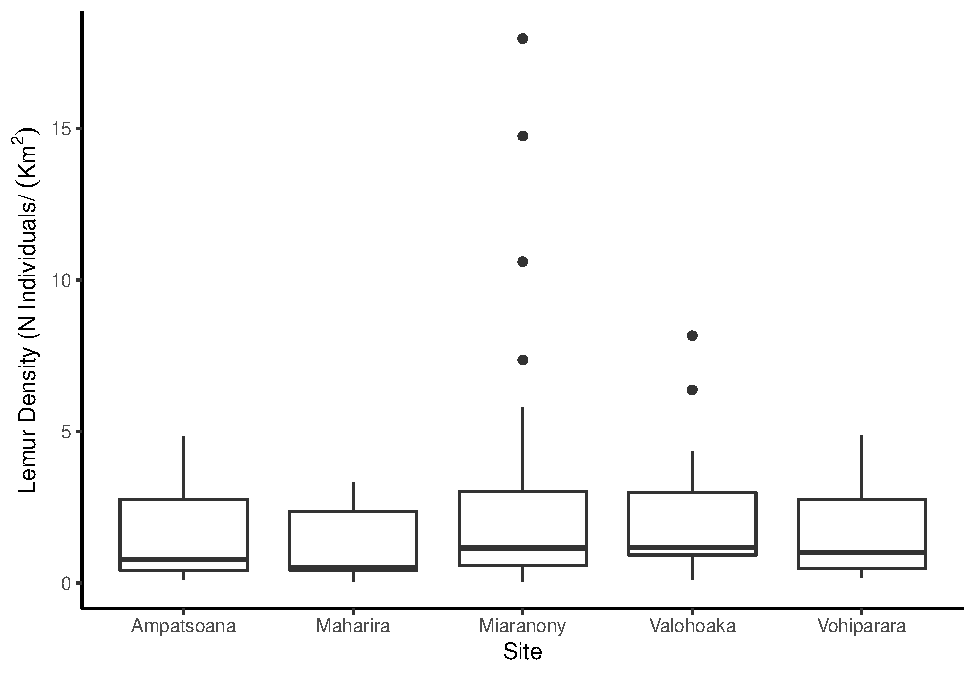
\includegraphics{project_draft_files/figure-latex/unnamed-chunk-8-1.pdf}
\caption{Figure 2. Boxplot of lemur densities at each sampling site.}
\end{figure}

\begin{Shaded}
\begin{Highlighting}[]
\FunctionTok{print}\NormalTok{(density\_aov\_plot2)}
\end{Highlighting}
\end{Shaded}

\begin{figure}
\centering
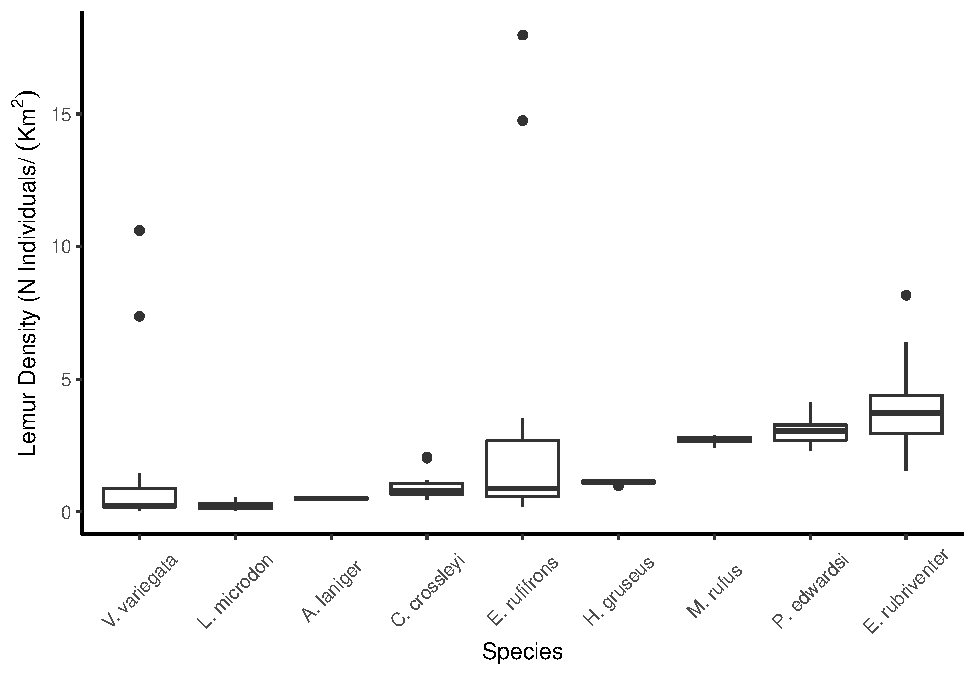
\includegraphics{project_draft_files/figure-latex/unnamed-chunk-9-1.pdf}
\caption{Figure 3. Boxplot of lemur densities for each species
surveyed.}
\end{figure}

Our best model with site as an independent vaiable demonstrates that
fruit nitrogen content, latitude, roughness, slope, fruit length, fruit
width, and the sites were significantly related to lemur density. This
model explains46.7\% of the variance in lemur density. With every
increase in one percentage of nitrogen on the log scale, lemur density
increases by 11.310 individuals per square Km (p = 0.007). With every
increase in one degree latitude, lemur density decreases by 28.030
individuals per square Km (p = 0.021). With every increase in one
roughness unit, lemur density decreases by 0.007 individuals per square
Km (p = 0.0.021). With every increase in one degree in slope, lemur
density increases by 0.259 individuals per square Km (p = 0.0294). Site
Maharira has 8.080 fewer lemurs per square Km (p = 0.275) when compared
to Ampatsona, whereas Valohoaka has 7.845 fewer (p = 0.0182) and
Vohiparara has 6.291 fewer (0.02026). With every increase in one mm of
mean fruit length on the log scale, lemur density increases by 8.711
individuals per square Km (p = 0.009). On the other hand, with every
increase in one mm of mean fruit width on the log scale, lemur density
decreases by 10.070 individuals per square Km (p = 0.002). When we
included site as a random variable, only nitrogen content, fruit length,
and fruit width were significantly related to lemur densities in the
best model. However, this model explained less variation in lemur
density (43.580\%) than the model where it was included as an
independent variable. With every increase in one percentage of mean
nitrogen on the log scale, lemur density increases by 7.758 individuals
per square Km (p = 0.002). With every increase in one mm of the mean
fruit length, lemur density increases by 7.737 individuals per square Km
(p = 0.00483). With every increase in one mm of the mean fruit width,
lemur density decreases by 6.512 individuals per square Km (p = 0.0117).

In our species-specific models, we identified that lemur specis differ
in their relationships to the habitat variables. Based on our best model
for \emph{Avahi laniger}, we found that log seed length, latitude, log
seed width, log SLA, site Maharira, site Valohoaka, site Vohiparara, log
fruit length, and log fruit width were related to the density of Avahi
laniger (p \textless{} 0.001). This model explains 82.4\% of variation
in density. The model for the \emph{Eulemur rubriventer} species
indicated that log nitrogen, log SLA, slope, SiteMaharira,
SiteMiaranony, SiteValohoaka (marginally), Site Vohiparara, log fruit
length, and log fruit width are relevant to \emph{Eulemur rubriventer}
densities (p = 0.002). This model explains 56.95\% of the variation in
the density data. The model for Lepilemur microdon indicated that log
nitrogen, log tannins (marginally), log SLA, slope, site Maharira, site
Valohoaka, log fruit length, and log fruit width are significantly
related to the density of this species (p \textless{} 0.001). The model
explained 97.13\% of the variability in density. The model for*
Propithecus edwardsi* indicated that latitude, log seed width, log
tannins, longitude, site Maharira, site Miaranony, siteValohoaka,
siteVohiparara, log fruit length, and log fruit width are relevant to
the densities of the species (p \textless{} 0.001). This model explained
about 75\% of the variability in the density of the species (Adjusted
R-squared: 0.7452).

\newpage

\hypertarget{summary-and-conclusions}{%
\section{Summary and Conclusions}\label{summary-and-conclusions}}

There is a significant difference in Lemur population density between
different species and between different sites. Although Miaranony and
Valohoaka have greater lemur densities than the other sites, this is
likely driven by outliers. Ampatsoana, Maharira, and Vohiparara all have
similar lemur densities. \emph{Eulemur rubriventer, Propithecus
edwardsi}, and \emph{Microcebus rufus} all tend to have higher densities
than the other lemur species, while \emph{Varecia variegata, Lepilemur
microdon, Avahi laniger}, and \emph{Cheirogaleus crossleyi} tend to have
lower densities. Our analyses demonstrate that these differences are
related to fruit length, nitrogen content, and fruit width. Latitude,
roughness, slope, and site also may be relevant, as indicated by the
best linear model created using species and transect site as the only
random effects. These results highlight the potential importance of
plant functional traits in driving patterns of lemur density across a
landscape. This is consistent with the literature; for example, lemur
population sizes are known to be related to the presence of fruiting
trees (Herrera et al.~2018). Latitude, roughness, and slope could also
be expected to influence which plant species occur in different sites.
However, differences in densities could also be reflective of life
history characteristics or other variables that were not included in
this study, such as human disturbance. These results could have
management implications. For example, it could be beneficial to focus
tree restoration efforts on species that contain the traits that are
positively related to lemur densities, such as nitrogen content. In
fact, restoration schemes based on lemur feeding trees have already been
proposed in Madagascar (Steffens et al.~2020). Fruit length and fruit
width are also related to lemur densities, although further studies
would be needed to determine which fruit sizes and lengths best support
various lemur species. Strategic decisions on which species to plant
based could be made based off of the length and width of fruit provided
by tree to best support the populations of specific lemur species.

Our analyses further demonstrated that the variables related to lemur
density differ between the various lemur species, although fruit width
and fruit length are related to the densities of each of the four
species we analyzed in depth. Fruit characteristics such as tannin
concentration, seed length, and seed width were relevant to the
densities of certain lemur species, while they weren't found to be
relevant to the densities of other lemur species. Similarly, landscape
characteristics such as slope and latitude were found to be relevant to
the densities of certain lemur species. The differences between the
models of the individual lemur species suggests that traits of the
lemurs might also be important in determining what habitat variables
relate to their densities. Lemurs vary greatly in their diets, habitat
preferences, and foraging ecology, and lemur social structure is related
to ecological variables (Overdorff 1996).

Future studies ought to integrate other variables into the analysis of
this question. For example, other studies could investigate how
functional traits and climatic variables interact with anthropogenic
disturbance to drive patterns in lemur densities. Human disturbance is
known to impact mammal population densities in the neotropics (Tucker et
al.~2021), so there might be similar dynamics in Madagascar. It would
also be interesting to incorporate lemur functional traits to analyze if
lemur diets, body sizes, and behavioral traits are significantly related
to their densities in a given area. Furthermore, a similar study at a
larger scale could be interesting because mouse lemur densities are
related to biogeographical variables (Setash et al.~2017), so it would
be interesting to identify the biogeogrphical variables that are related
to other species. \newpage

\hypertarget{references}{%
\section{References}\label{references}}

Barton, K. (2020). MuMIn: Multi-Model Inference. R package version
1.43.17. \url{https://CRAN.R-project.org/package=MuMIn}

Bates, D., Maechler, M., Bolker, B., Walker, S. (2015). Fitting Linear
Mixed-Effects Models Using lme4. Journal of Statistical Software, 67(1),
1-48. \url{doi:10.18637/jss.v067.i01}

Brown, K. A., Parks, K. E., Bethell, C. A., Johnson, S. E., \& Mulligan,
M. (2015). Predicting Plant Diversity Patterns in Madagascar:
Understanding the Effects of Climate and Land Cover Change in a
Biodiversity Hotspot. PLOS ONE, 10(4), e0122721.
\url{https://doi.org/10.1371/journal.pone.0122721}

De Mendiburu, F. (2020). agricolae: Statistical Procedures for
Agricultural Research. R package version 1.3-3.
\url{https://CRAN.R-project.org/package=agricolae}

Donati, G., Santini, L., Eppley, T. M., Arrigo-Nelson, S. J., Balestri,
M., Boinski, S., Bollen, A., Bridgeman, L. L., Campera, M., Carrai, V.,
Chalise, M. K., Derby Lewis, A., Hohmann, G., Kinnaird, M. F., Koenig,
A., Kowalewski, M., Lahann, P., McLennan, M. R., Nekaris, A. K. I.,
\ldots{} Ganzhorn, J. U. (2017). Low Levels of Fruit Nitrogen as Drivers
for the Evolution of Madagascar's Primate Communities. Scientific
Reports, 7(1), 14406. \url{https://doi.org/10.1038/s41598-017-13906-y}

Fiske, I., Chandler, R. (2011). unmarked: An R Package for Fitting
Hierarchical Models of Wildlife Occurrence and Abundance. Journal of
Statistical Software, 43(10), 1-23. URL
\url{http://www.jstatsoft.org/v43/i10/}.

Herrera, J. P., Borgerson, C., Tongasoa, L., Andriamahazoarivosoa, P.,
Rasolofoniaina, B. J. R., Rakotondrafarasata, E. R., Randrianasolo, J.
L. R. R., Johnson, S. E., Wright, P. C., \& Golden, C. D. (2018).
Estimating the population size of lemurs based on their mutualistic food
trees. Journal of Biogeography, 45(11), 2546--2563.
\url{https://doi.org/10.1111/jbi.13409}

Kuznetsova, A., Brockhoff, P.B., Christensen, R.H.B. (2017). ``lmerTest
Package: Tests in Linear Mixed Effects Models.'' \emph{Journal of
Statistical Software}, \emph{82}(13), 1-26. doi: 10.18637/jss.v082.i13
(URL: \url{https://doi.org/10.18637/jss.v082.i13}).

Lim, J. Y., Svenning, J.-C., Göldel, B., Faurby, S., \& Kissling, W. D.
(2020). Frugivore-fruit size relationships between palms and mammals
reveal past and future defaunation impacts. Nature Communications,
11(1), 4904. \url{https://doi.org/10.1038/s41467-020-18530-5}

Park, D. S., \& Razafindratsima, O. H. (2019). Anthropogenic threats can
have cascading homogenizing effects on the phylogenetic and functional
diversity of tropical ecosystems. Ecography, 42(1), 148--161.
\url{https://doi.org/10.1111/ecog.03825}

Overdorff, D. J. (1996). Ecological correlates to social structure in
two lemur species in Madagascar. American Journal of Physical
Anthropology, 100(4), 487--506.
\url{https://doi.org/10.1002/(SICI)1096-8644(199608)100:4}\textless487::AID-AJPA4\textgreater3.0.CO;2-O

Razafindratsima, O. H., Mehtani, S., \& Dunham, A. E. (2013).
Extinctions, traits and phylogenetic community structure: Insights from
primate assemblages in Madagascar. Ecography, 36(1), 47--56.
\url{https://doi.org/10.1111/j.1600-0587.2011.07409.x}

Schwitzer, C., Mittermeier, R. A., Johnson, S. E., Donati, G., Irwin,
M., Peacock, H., \ldots{} \& Wright, P. C. (2014). Averting lemur
extinctions amid Madagascar's political crisis. Science, 343(6173),
842-843.

Setash, C. M., Zohdy, S., Gerber, B. D., \& Karanewsky, C. J. (2017). A
biogeographical perspective on the variation in mouse lemur density
throughout Madagascar. Mammal Review, 47(3), 212--229.
\url{https://doi.org/10.1111/mam.12093}

Steffens, K. J. E. (2020). Lemur food plants as options for forest
restoration in Madagascar. Restoration Ecology, 28(6), 1517--1527.
\url{https://doi.org/10.1111/rec.13234}

Valenta, K., Burke, R. J., Styler, S. A., Jackson, D. A., Melin, A. D.,
\& Lehman, S. M. (2013). Colour and odour drive fruit selection and seed
dispersal by mouse lemurs. Scientific Reports (Nature Publisher Group),
3, 2424. \url{http://dx.doi.org.proxy.lib.duke.edu/10.1038/srep02424}

Wright, P., Razafindratsita, V., Pochron, S., \& Jernvall, J. (1970).
The Key to Madagascar Frugivores. In Tropical Fruits and Frugivores: The
Search for Strong Interactors (pp.~121--138).
\url{https://doi.org/10.1007/1-4020-3833-X_7}

Zeileis, A. Hothorn, T. (2002). Diagnostic Checking in Regression
Relationships. R News 2(3), 7-10. URL
\url{https://CRAN.R-project.org/doc/Rnews/}

Wickham, H. ggplot2: Elegant Graphics for Data Analysis. Springer-Verlag
New York, 2016.

\end{document}
